\subsubsection{UC1 Caso d'uso pubblico}
\begin{figure}[H]
\centering
\noindent\makebox[\textwidth]{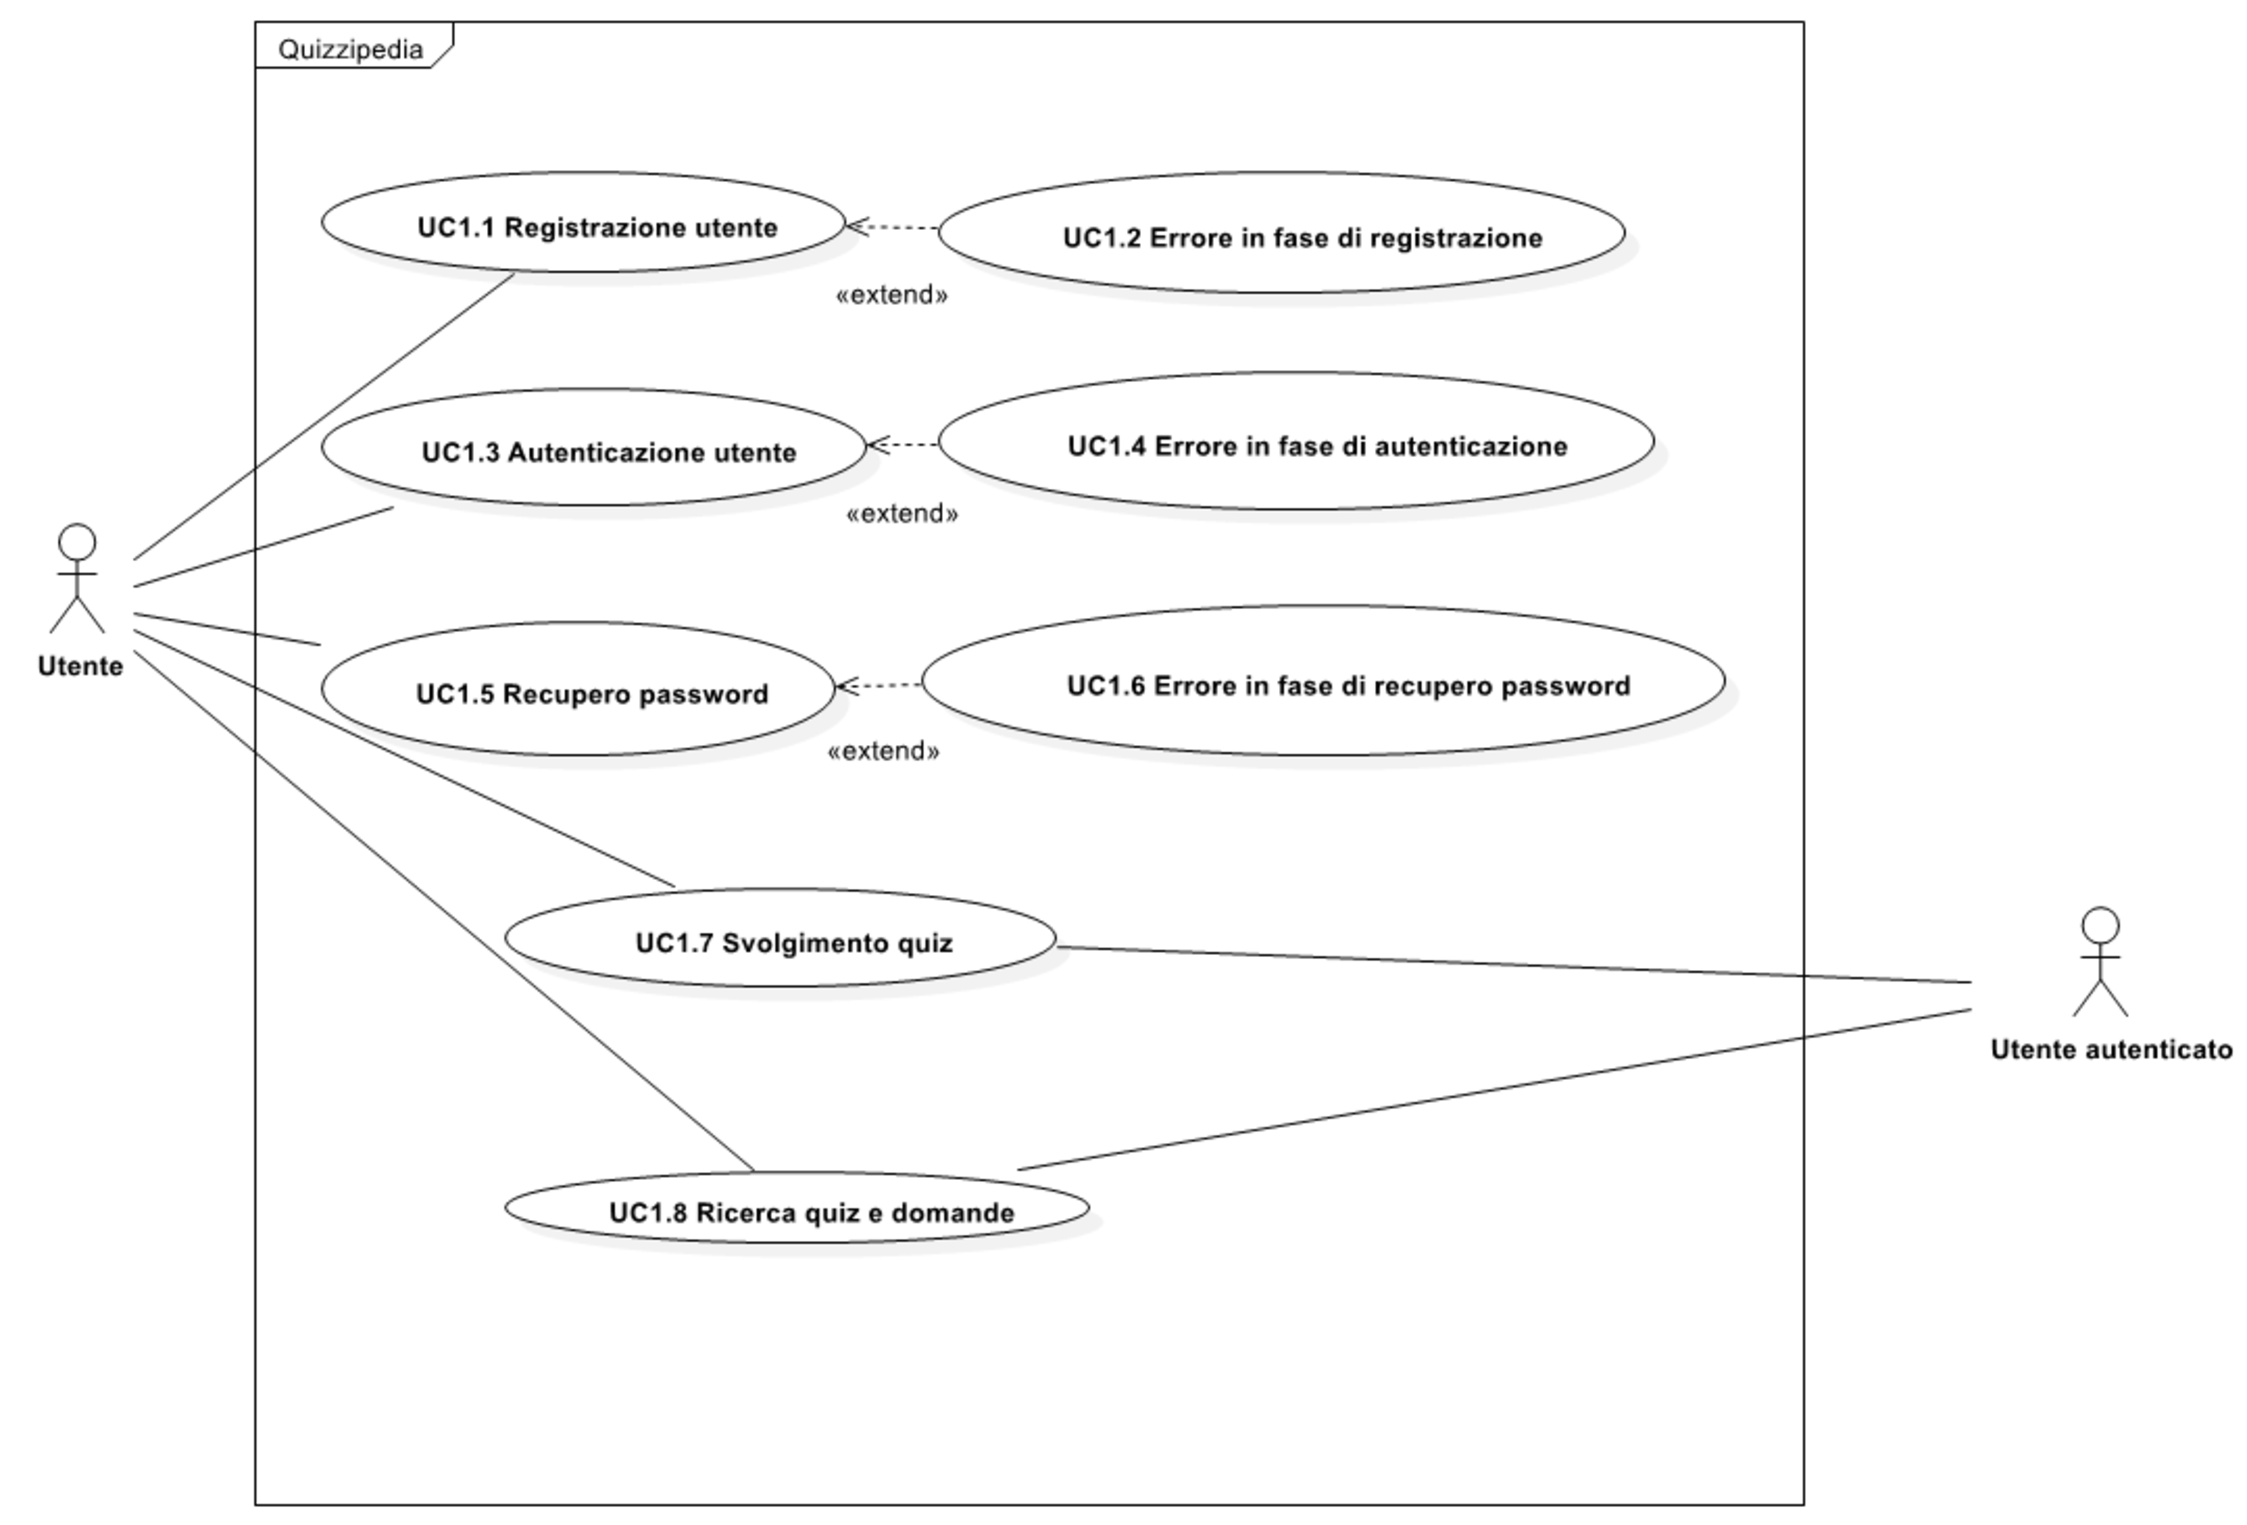
\includegraphics[width=\textwidth]{Img/UC Caso d'uso pubblico.pdf}}
\caption{UC1 Caso d'uso pubblico}
\end{figure}
\begin{itemize}
\item \textbf{Attori}: Utente, Utente Autenticato.
\item \textbf{Scenario principale}:
\begin{enumerate}
\item Registrazione utente (UC1.1);
\item Errore in fase di registrazione (UC1.2);
\item Autenticazione utente (UC1.3);
\item Errore in fase di autenticazione (UC1.4);
\item Recupero password (UC1.5);
\item Errore in fase di recupero password (UC1.6);
\item Svolgimento quiz (UC1.7);
\item Ricerca quiz e domande (UC1.8).
\end{enumerate}
\item \textbf{Descrizione}: l'utente accede al sito. Può effettuare la registrazione, autenticarsi nel sistema, effettuare il recupero della propria password, cercare quiz e domande, svolgere quiz.
\item \textbf{Precondizione}: l'utente si è connesso al sito web di Quizzipedia attraverso un browser supportato.
\item \textbf{Postcondizione}: l'utente ha scelto l'operazione da intraprendere.
\end{itemize}
\subsubsection{UC1.1 Registrazione utente}
\begin{figure}[H]
\centering
\noindent\makebox[\textwidth]{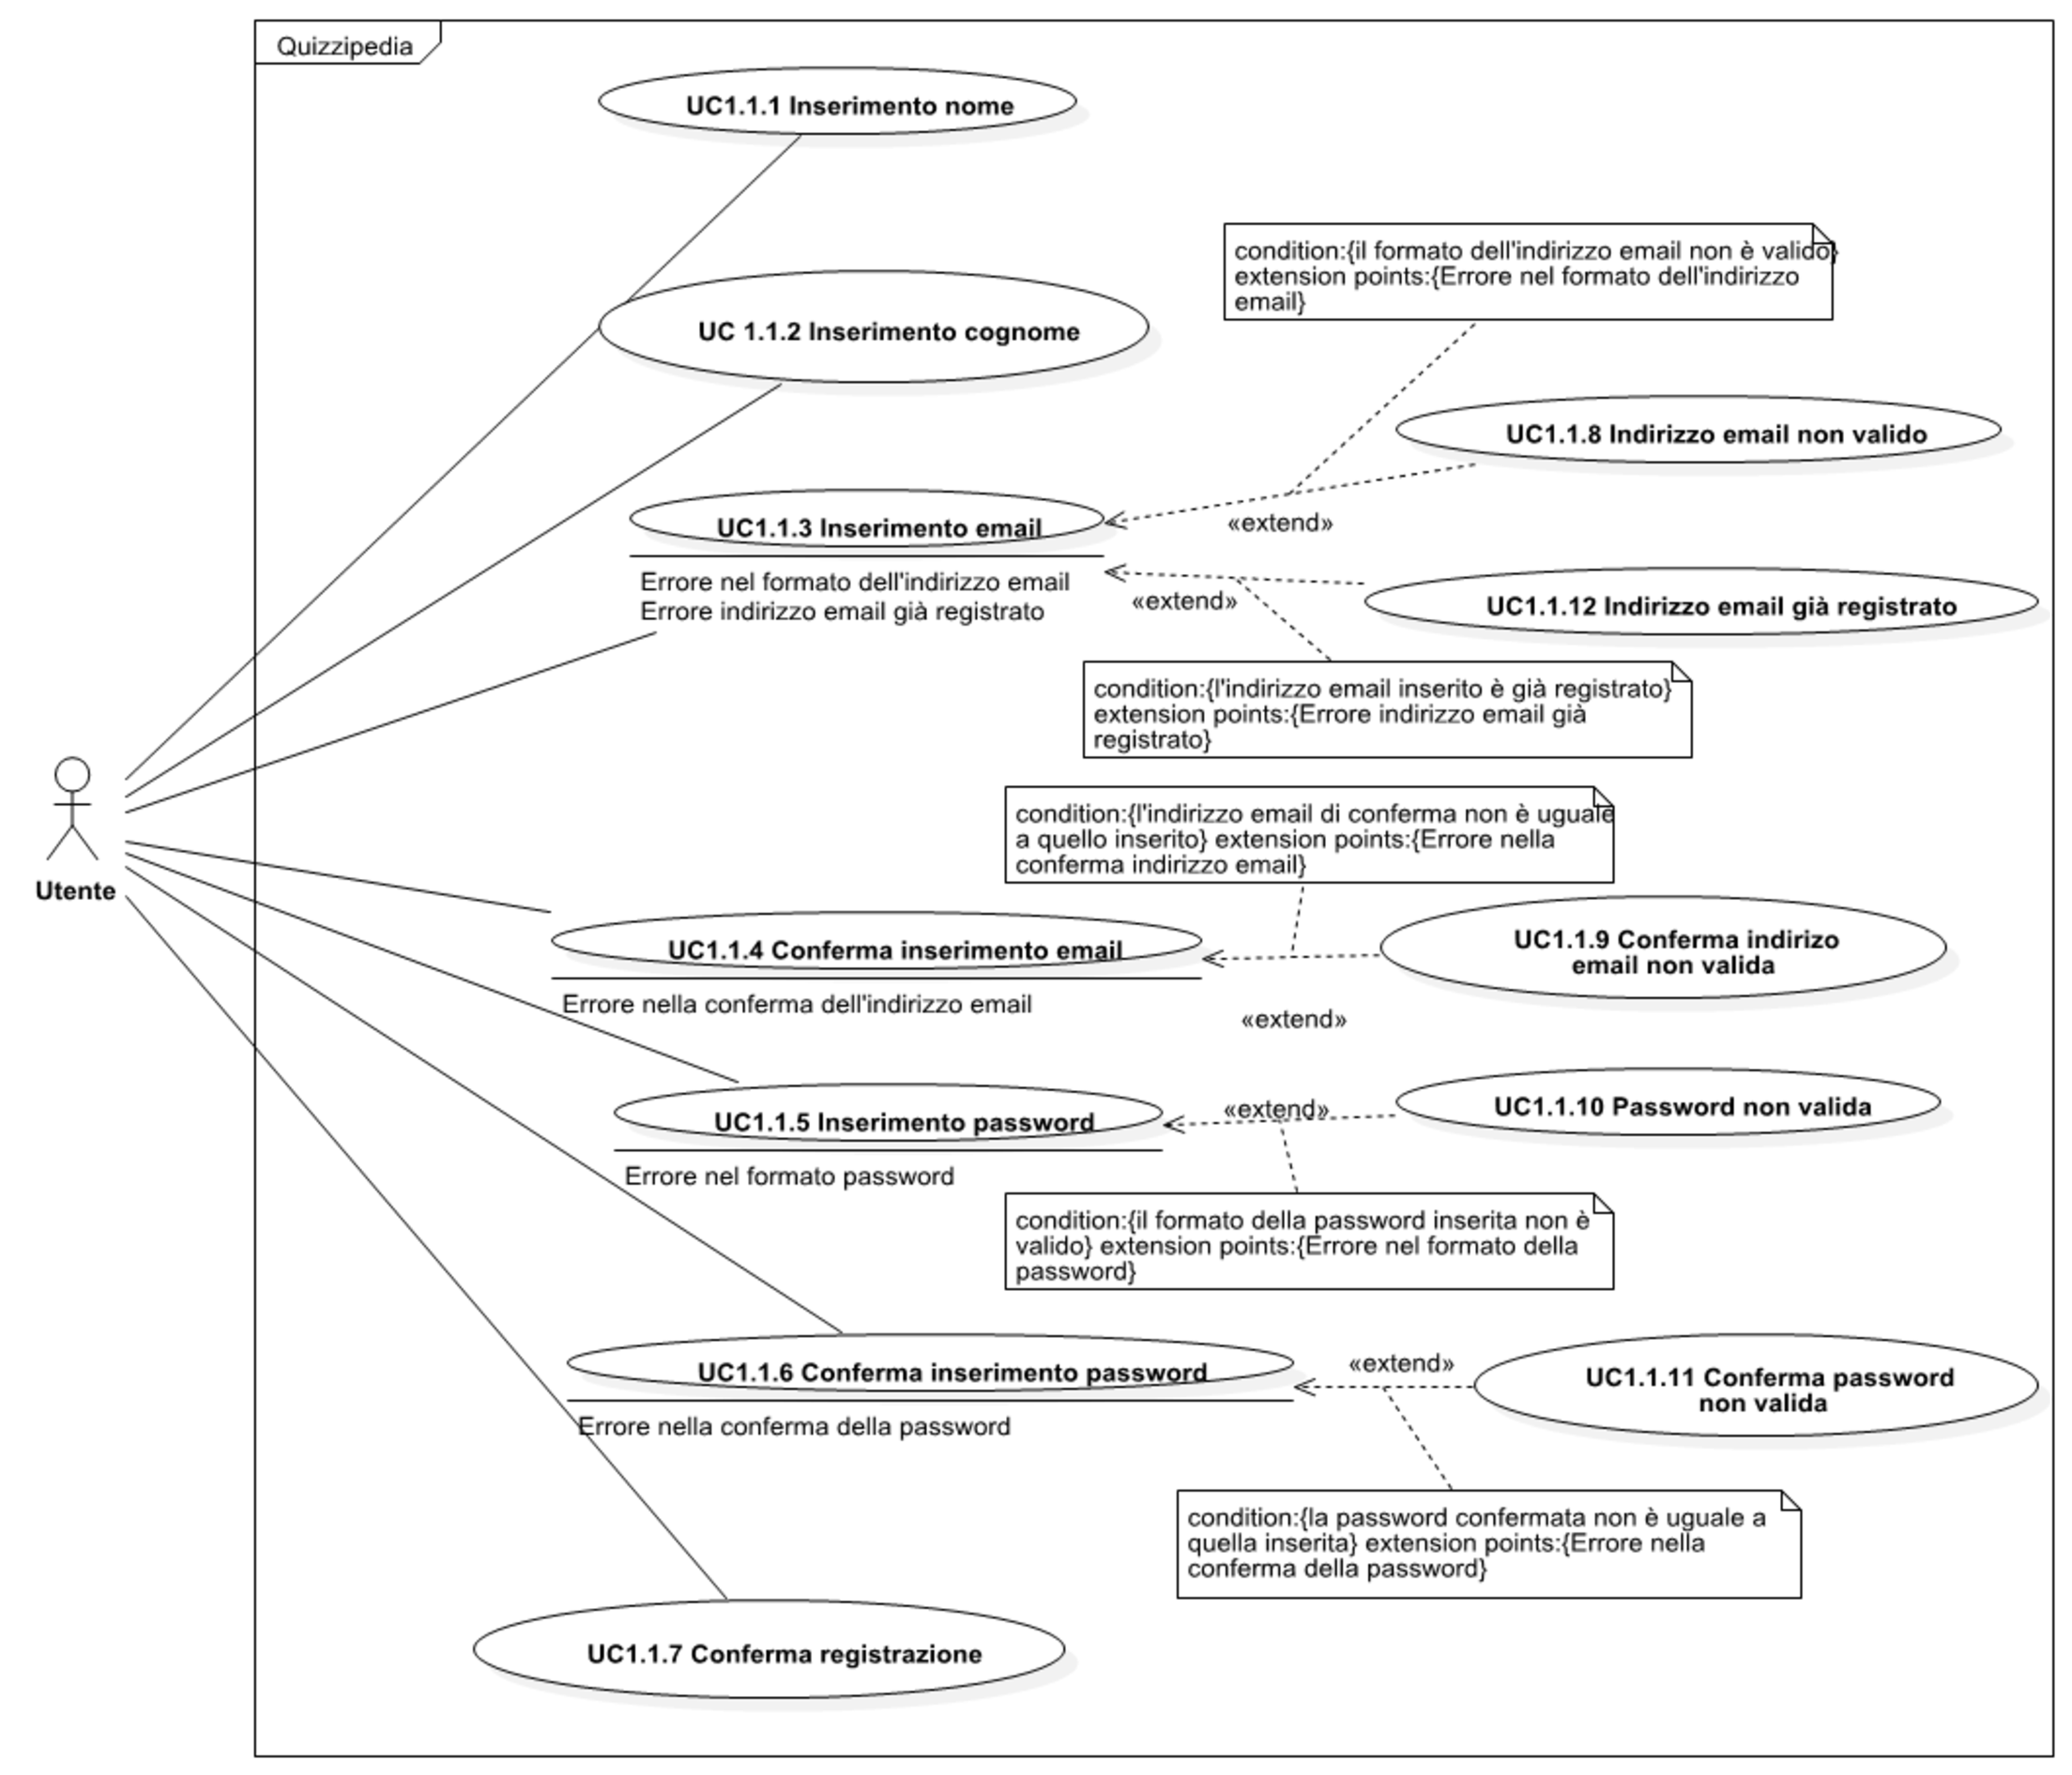
\includegraphics[width=\textwidth]{Img/UC Registrazione utente.pdf}}
\caption{UC1.1 Registrazione utente}
\end{figure}
\begin{itemize}
\item \textbf{Attori}: Utente.
\item \textbf{Scenario principale}:
\begin{enumerate}
\item Inserimento nome (UC1.1.1);
\item Inserimento cognome (UC1.1.2);
\item Inserimento email (UC1.1.3);
\item Conferma inserimento email (UC1.1.4);
\item Inserimento password (UC1.1.5);
\item Conferma inserimento password (UC1.1.6);
\item Conferma registrazione (UC1.1.7).
\end{enumerate}
\item \textbf{Scenario alternativo}: l'utente interrompe volontariamente la registrazione.
\item \textbf{Estensioni}:
\begin{itemize}
\item Errore in fase di registrazione (UC1.2).
\end{itemize}
\item \textbf{Descrizione}: l'utente crea un account Quizzipedia per poter usufruire delle funzionalità offerte dal sistema agli utenti registrati.
\item \textbf{Precondizione}: l'utente si è connesso al sito web di Quizzipedia attraverso un browser supportato e ha scelto di effettuare la registrazione.
\item \textbf{Postcondizione}: l'utente è stato registrato nel sistema con i dati immessi.
\end{itemize}
\subsubsection{UC1.1.1 Inserimento nome}
\begin{itemize}
\item \textbf{Attori}: Utente.
\item \textbf{Descrizione}: per portare a termine la registrazione, l'utente deve inserire il proprio nome.
\item \textbf{Precondizione}: l'utente si trova nella pagina di registrazione e deve ancora inserire il proprio nome.
\item \textbf{Postcondizione}: l'utente ha inserito il nome.
\end{itemize}
\subsubsection{UC1.1.2 Inserimento cognome}
\begin{itemize}
\item \textbf{Attori}: Utente.
\item \textbf{Descrizione}: per portare a termine la registrazione, l'utente deve inserire il proprio cognome.
\item \textbf{Precondizione}: l'utente si trova nella pagina di registrazione e deve ancora inserire il proprio cognome.
\item \textbf{Postcondizione}: l'utente ha inserito il cognome.
\end{itemize}
\subsubsection{UC1.1.3 Inserimento email}
\begin{itemize}
\item \textbf{Attori}: Utente.
\item \textbf{Scenario alternativo}: l'indirizzo email non è valido e deve essere inserito nuovamente.
\item \textbf{Descrizione}: per portare a termine la registrazione, l'utente deve inserire il proprio indirizzo email.
\item \textbf{Precondizione}: l'utente si trova nella pagina di registrazione e deve ancora inserire l'indirizzo email.
\item \textbf{Postcondizione}: l'utente ha inserito un indirizzo email valido.
\end{itemize}
\subsubsection{UC1.1.4 Conferma inserimento email}
\begin{itemize}
\item \textbf{Attori}: Utente.
\item \textbf{Scenario alternativo}: l'indirizzo email non è uguale a quello precedentemente inserito.
\item \textbf{Descrizione}: per portare a termine la registrazione, l'utente deve confermare il proprio indirizzo email.
\item \textbf{Precondizione}: l'utente si trova nella pagina di registrazione, ha inserito l'indirizzo email e deve ancora confermarlo.
\item \textbf{Postcondizione}: l'utente ha confermato un indirizzo email valido e uguale a quello inserito.
\end{itemize}
\subsubsection{UC1.1.5 Inserimento password}
\begin{itemize}
\item \textbf{Attori}: Utente.
\item \textbf{Scenario alternativo}: la password inserita non è valida e quindi deve essere inserita nuovamente.
\item \textbf{Descrizione}: per portare a termine la registrazione, l'utente deve inserire la propria password.
\item \textbf{Precondizione}: l'utente si trova nella pagina di registrazione e deve ancora inserire la password.
\item \textbf{Postcondizione}: l'utente ha inserito una password valida.
\end{itemize}
\subsubsection{UC1.1.6 Conferma inserimento password}
\begin{itemize}
\item \textbf{Attori}: Utente.
\item \textbf{Scenario alternativo}: la password non è uguale a quella precedentemente inserita.
\item \textbf{Descrizione}: per portare a termine la registrazione, l'utente deve confermare la propria password.
\item \textbf{Precondizione}: l'utente si trova nella pagina di registrazione, ha inserito la password e deve ancora confermarla.
\item \textbf{Postcondizione}: l'utente ha confermato una password valida e uguale a quella inserita.
\end{itemize}
\subsubsection{UC1.1.7 Conferma registrazione}
\begin{itemize}
\item \textbf{Attori}: Utente.
\item \textbf{Descrizione}: per portare a termine la registrazione, l'utente deve confermare i dati precedentemente inseriti.
\item \textbf{Precondizione}: l'utente si trova in una pagina del sito web che gli permette di confermare i dati precedentemente inseriti.
\item \textbf{Postcondizione}: L'utente ha scelto di continuare la registrazione con i dati immessi.
\end{itemize}
\subsubsection{UC1.2 Errore in fase di registrazione}
\begin{itemize}
\item \textbf{Attori}: Utente.
\item \textbf{Descrizione}: si è verificata una delle seguenti condizioni: l'indirizzo email inserito è già associato ad un account registrato, l'indirizzo email inserito non è in un formato valido, l'indirizzo email di conferma non corrisponde a quello precedentemente inserito, la password inserita non è conforme (troppo corta, troppo semplice), la password di conferma non corrisponde a quella precedentemente inserita.
\item \textbf{Precondizione}: l'utente ha effettuato un tentativo di registrazione che non è andato a buon termine.
\item \textbf{Postcondizione}: l'utente ha visualizzato il messaggio di errore.
\end{itemize}
\subsubsection{UC1.3 Autenticazione utente}
\begin{figure}[H]
\centering
\noindent\makebox[\textwidth]{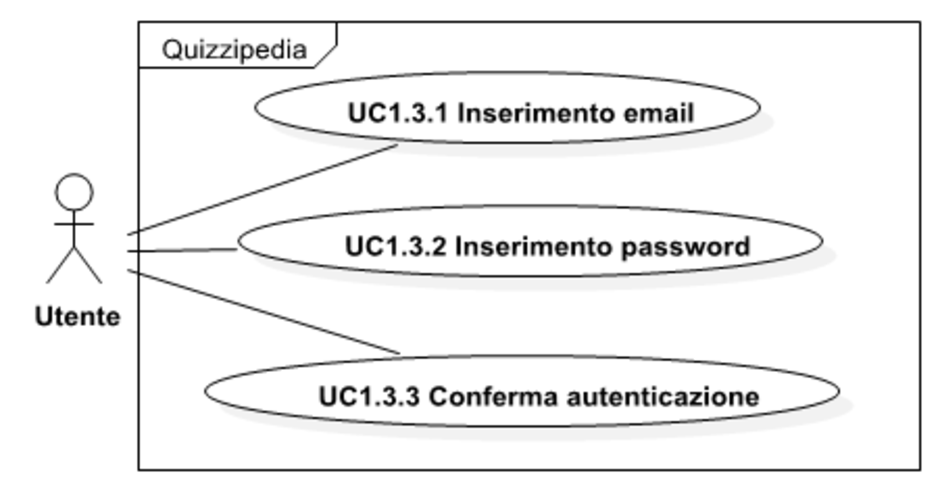
\includegraphics[width=\textwidth]{Img/UC Autenticazione utente.pdf}}
\caption{UC1.3 Autenticazione utente}
\end{figure}
\begin{itemize}
\item \textbf{Attori}: Utente.
\item \textbf{Scenario principale}:
\begin{enumerate}
\item Inserimento email (UC1.3.1);
\item Inserimento password (UC1.3.2);
\item Conferma autenticazione (UC1.3.3).
\end{enumerate}
\item \textbf{Scenario alternativo}: l'utente interrompe volontariamente l'autenticazione.
\item \textbf{Estensioni}:
\begin{itemize}
\item Errore in fase di autenticazione (UC1.4).
\end{itemize}
\item \textbf{Descrizione}: l'utente, se in possesso di un account Quizzipedia, deve avere la possibilità di autenticarsi.
\item \textbf{Precondizione}: l'utente si è connesso al sito web di Quizzipedia attraverso un browser supportato e ha scelto di effettuare l'autenticazione.
\item \textbf{Postcondizione}: il sistema ha autenticato l'utente.
\end{itemize}
\subsubsection{UC1.3.1 Inserimento email}
\begin{itemize}
\item \textbf{Attori}: Utente.
\item \textbf{Descrizione}: per portare a termine l'autenticazione, l'utente deve inserire il proprio indirizzo.
\item \textbf{Precondizione}: l'utente si trova in una pagina di autenticazione e deve ancora inserire il proprio indirizzo email.
\item \textbf{Postcondizione}: l'utente ha inserito il proprio indirizzo email.
\end{itemize}
\subsubsection{UC1.3.2 Inserimento password}
\begin{itemize}
\item \textbf{Attori}: Utente.
\item \textbf{Descrizione}: per portare a termine l'autenticazione, l'utente deve inserire la password.
\item \textbf{Precondizione}: l'utente si trova in una pagina di autenticazione e deve ancora inserire la password.
\item \textbf{Postcondizione}: l'utente ha inserito la password.
\end{itemize}
\subsubsection{UC1.3.3 Conferma autenticazione}
\begin{itemize}
\item \textbf{Attori}: Utente.
\item \textbf{Descrizione}: per portare a termine l'autenticazione, l'utente deve confermare l'autenticazione con l'indirizzo email e  la password immessi.
\item \textbf{Precondizione}: l'utente si trova in una pagina del sito web che gli permette di confermare l'autenticazione.
\item \textbf{Postcondizione}: l'utente ha scelto di continuare l'autenticazione con i dati immessi.
\end{itemize}
\subsubsection{UC1.4 Errore in fase di autenticazione}
\begin{itemize}
\item \textbf{Attori}: Utente.
\item \textbf{Descrizione}: si è verificata una delle seguenti condizioni: l'indirizzo email inserito non è associato a un account registrato, oppure la combinazione di indirizzo email e password immessa è errata.
\item \textbf{Precondizione}: l'utente ha effettuato un tentativo di autenticazione che non è andato a buon termine.
\item \textbf{Postcondizione}: l'utente ha visualizzato il messaggio di errore.
\end{itemize}
\subsubsection{UC1.5 Recupero password}
\begin{figure}[H]
\centering
\noindent\makebox[\textwidth]{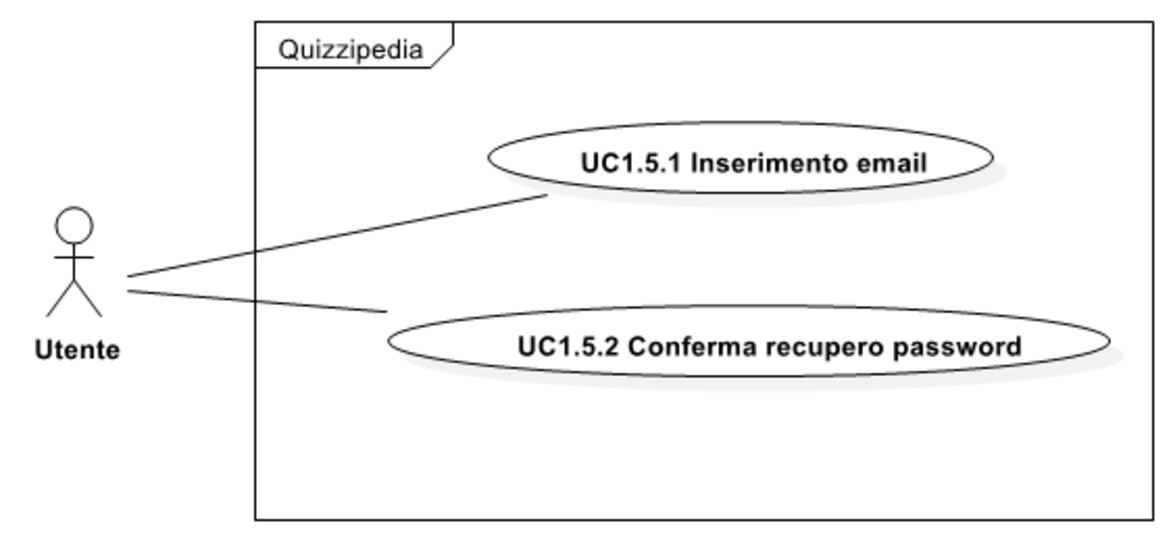
\includegraphics[width=\textwidth]{Img/UC Recupero password.pdf}}
\caption{UC1.5 Recupero password}
\end{figure}
\begin{itemize}
\item \textbf{Attori}: Utente.
\item \textbf{Scenario principale}:
\begin{enumerate}
\item Inserimento email (UC1.5.1);
\item Conferma recupero password (UC1.5.2).
\end{enumerate}
\item \textbf{Estensioni}:
\begin{itemize}
\item Errore in fase di recupero password (UC1.6).
\end{itemize}
\item \textbf{Descrizione}: l'utente in possesso di un account Quizzipedia deve avere la possibilità di accedere al sistema anche in caso di dimenticanza della propria password, a patto che ricordi l'indirizzo email a cui è associato il suo account.
\item \textbf{Precondizione}: l'utente si è connesso al sito web di Quizzipedia attraverso un browser supportato e vuole recuperare l'accesso al proprio account Quizzipedia.
\item \textbf{Postcondizione}: l'utente ha recuperato l'accesso al proprio account Quizzipedia.
\end{itemize}
\subsubsection{UC1.5.1 Inserimento email}
\begin{itemize}
\item \textbf{Attori}: Utente.
\item \textbf{Descrizione}: per portare a termine l'operazione, l'utente deve inserire il proprio indirizzo email. Se l'indirizzo email è associato a un account registrato, gli verrà inviata una password temporanea o un link che consentirà all'utente di scegliere una nuova password senza dover ricordare la vecchia.
\item \textbf{Precondizione}: l'utente si trova nella pagina di recupero password e deve ancora inserire l'indirizzo email.
\item \textbf{Postcondizione}: l'utente ha inserito il proprio indirizzo email.
\end{itemize}
\subsubsection{UC1.5.2 Conferma recupero password}
\begin{itemize}
\item \textbf{Attori}: Utente.
\item \textbf{Descrizione}: per portare a termine il recupero password, l'utente deve confermare l'operazione con l'indirizzo email immesso.
\item \textbf{Precondizione}: l'utente si trova in una pagina del sito web che gli permette di confermare il recupero password.
\item \textbf{Postcondizione}: l'utente ha scelto di continuare il recupero password con l'indirizzo email immesso.
\end{itemize}
\subsubsection{UC1.6 Errore in fase di recupero password}
\begin{itemize}
\item \textbf{Attori}: Utente.
\item \textbf{Descrizione}: si è verificata la seguente condizione: l'indirizzo email inserito non è associato a un account registrato.
\item \textbf{Precondizione}: l'utente ha effettuato un tentativo di recupero password che non è andato a buon termine.
\item \textbf{Postcondizione}: l'utente ha visualizzato il messaggio di errore.
\end{itemize}
\subsubsection{UC1.7 Svolgimento quiz}
\begin{figure}[H]
\centering
\noindent\makebox[\textwidth]{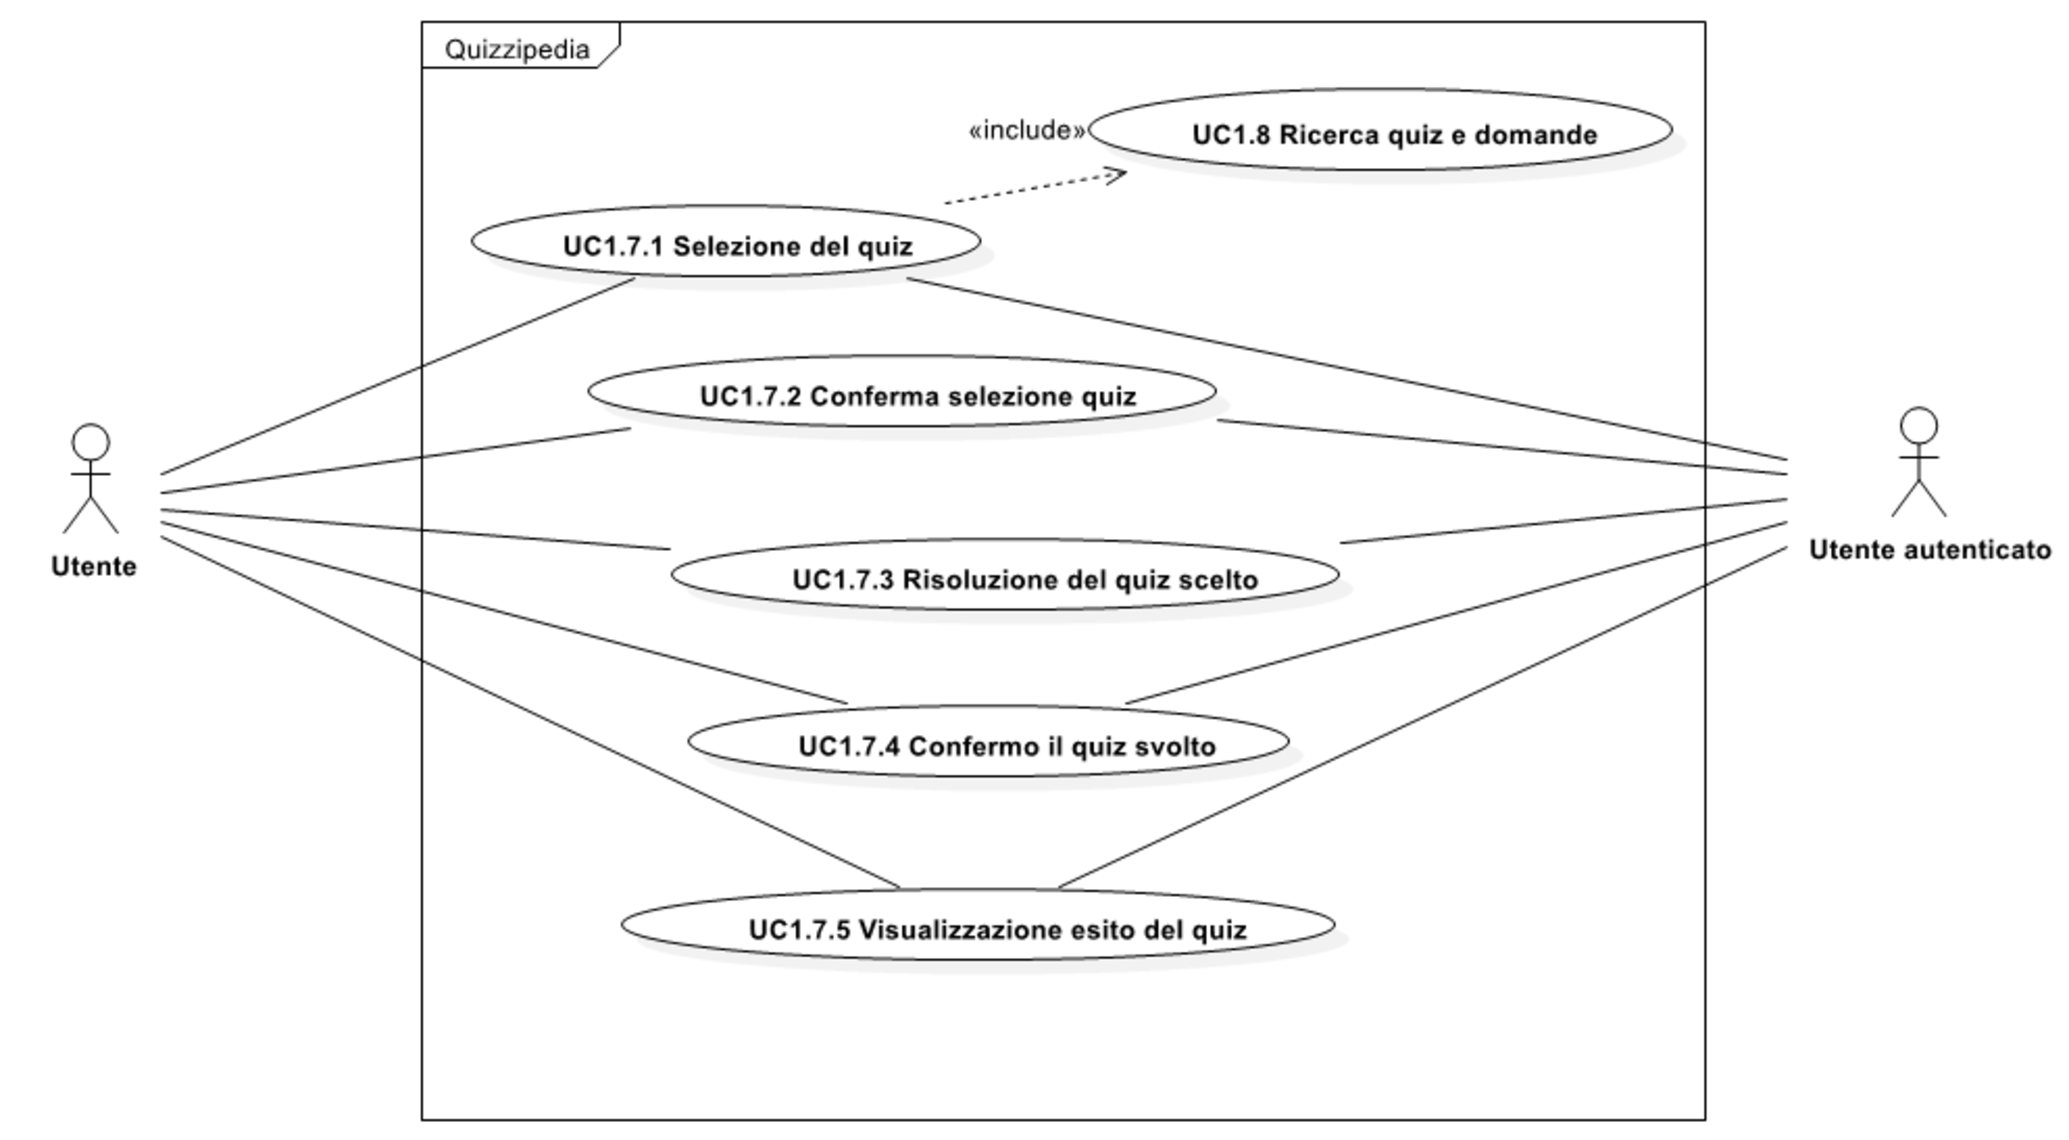
\includegraphics[width=\textwidth]{Img/UC Svolgimento quiz.pdf}}
\caption{UC1.7 Svolgimento quiz}
\end{figure}
\begin{itemize}
\item \textbf{Attori}: Utente, Utente Autenticato.
\item \textbf{Scenario principale}:
\begin{enumerate}
\item Selezione quiz (UC1.7.1);
\item Conferma selezione quiz (UC1.7.2);
\item Risoluzione quiz scelto (UC1.7.3);
\item Conferma risoluzione quiz (UC1.7.4);
\item Visualizzazione esito del quiz (UC1.7.5).
\end{enumerate}
\item \textbf{Scenario alternativo}: l'utente ha interrotto lo svolgimento del quiz.
\item \textbf{Descrizione}: l'utente deve poter svolgere un quiz conforme ai permessi dell'utente.
\item \textbf{Precondizione}: l'utente ha scelto di svolgere un quiz.
\item \textbf{Postcondizione}: l'utente ha finito di svolgere un quiz.
\end{itemize}
\subsubsection{UC1.7.1 Selezione quiz}
\begin{itemize}
\item \textbf{Attori}: Utente, Utente Autenticato.
\item \textbf{Inclusioni}:
\begin{itemize}
\item Ricerca quiz e domande (UC1.8).
\end{itemize}
\item \textbf{Descrizione}: l'utente deve poter selezionare il quiz che intende svolgere.
\item \textbf{Precondizione}: l'utente ha scelto di svolgere un quiz e vuole selezionarne uno.
\item \textbf{Postcondizione}: l'utente ha selezionato il quiz.
\end{itemize}
\subsubsection{UC1.7.2 Conferma selezione quiz}
\begin{itemize}
\item \textbf{Attori}: Utente, Utente Autenticato.
\item \textbf{Descrizione}: l'utente deve confermare la selezione del quiz scelto per iniziarne lo svolgimento.
\item \textbf{Precondizione}: l'utente ha selezionato il quiz da svolgere e deve confermarlo.
\item \textbf{Postcondizione}: l'utente ha confermato la selezione del quiz.
\end{itemize}
\subsubsection{UC1.7.3 Risoluzione quiz scelto}
\begin{itemize}
\item \textbf{Attori}: Utente, Utente Autenticato.
\item \textbf{Descrizione}: l'utente deve poter svolgere il quiz che ha selezionato, una domanda alla volta. È possibile spostarsi a piacimento fra le domande e rispondere a una domanda più volte, l'ultima risposta sovrascrive le precedenti.
\item \textbf{Precondizione}: l'utente ha selezionato e confermato un quiz da svolgere.
\item \textbf{Postcondizione}: l'utente ha concluso la risoluzione del quiz.
\end{itemize}
\subsubsection{UC1.7.4 Conferma risoluzione quiz}
\begin{itemize}
\item \textbf{Attori}: Utente, Utente Autenticato.
\item \textbf{Descrizione}: l'utente deve poter confermare la risoluzione del quiz, terminandne così lo svolgimento. Una volta confermata la risoluzione non sarà più possibile modificare le risposte.
\item \textbf{Precondizione}:  l'utente ha terminato la risoluzione del quiz e vuole riceverne l'esito.
\item \textbf{Postcondizione}: l'utente ha confermato la risoluzione del quiz con le risposte date.
\end{itemize}
\subsubsection{UC1.7.5 Visualizzazione esito del quiz}
\begin{itemize}
\item \textbf{Attori}: Utente, Utente Autenticato.
\item \textbf{Descrizione}: l'utente deve poter visualizzare l'esito del quiz svolto. L'esito può comprendere: il voto ricevuto, la soluzione corretta delle domande a cui è stata data una risposta errata.
\item \textbf{Precondizione}: l'utente ha confermato la risoluzione del quiz svolto.
\item \textbf{Postcondizione}: l'utente ha visualizzato l'esito.
\end{itemize}
\subsubsection{UC1.8 Ricerca quiz e domande}
\begin{figure}[H]
\centering
\noindent\makebox[\textwidth]{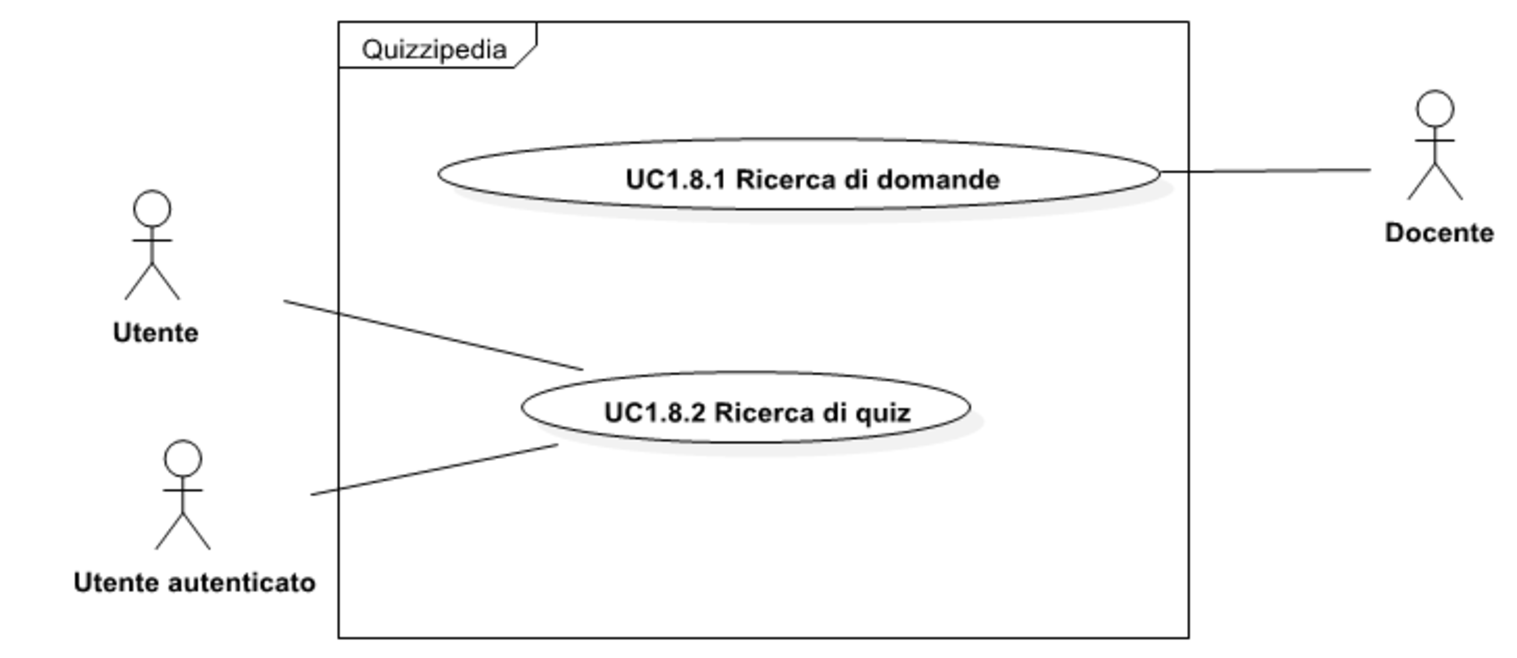
\includegraphics[width=\textwidth]{Img/UC Ricerca quiz e domande.pdf}}
\caption{UC1.8 Ricerca quiz e domande}
\end{figure}
\begin{itemize}
\item \textbf{Attori}: Utente, Utente Autenticato.
\item \textbf{Scenario principale}:
\begin{enumerate}
\item Selezione parametri di ricerca (UC1.8.1);
\item Conferma inizio ricerca (UC1.8.2);
\item Visualizzazione lista risultati (UC1.8.3).
\end{enumerate}
\item \textbf{Scenario alternativo}: l'utente ha interrotto la ricerca.
\item \textbf{Descrizione}: l'utente può effettuare una ricerca di quiz e domande presenti nel sistema. La ricerca è personalizzabile attraverso vari parametri di ricerca.
\item \textbf{Precondizione}: l'utente desidera effettuare una ricerca di quiz e domande.
\item \textbf{Postcondizione}: l'utente ha effettuato la ricerca.
\end{itemize}
\subsubsection{UC1.8.1 Selezione parametri di ricerca}
\begin{figure}[H]
\centering
\noindent\makebox[\textwidth]{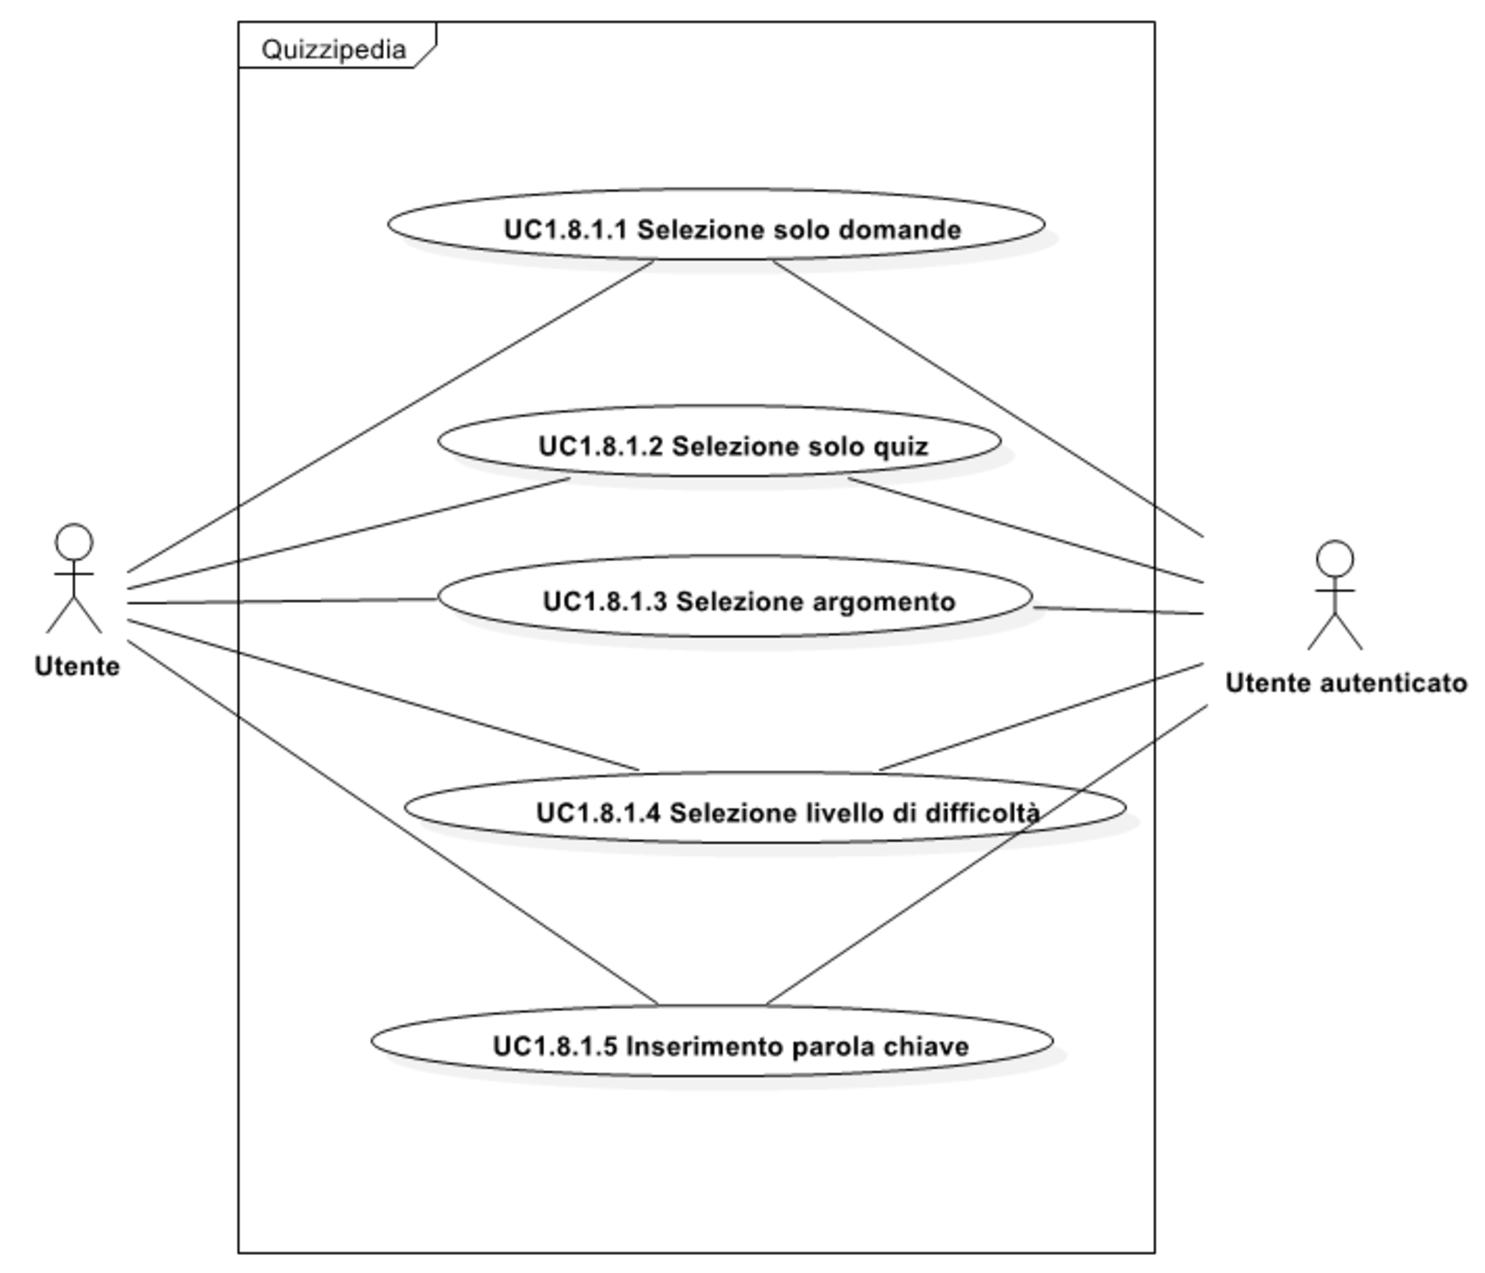
\includegraphics[width=\textwidth]{Img/UC Selezione parametri di ricerca.pdf}}
\caption{UC1.8.1 Selezione parametri di ricerca}
\end{figure}
\begin{itemize}
\item \textbf{Attori}: Utente, Utente Autenticato.
\item \textbf{Scenario principale}:
\begin{enumerate}
\item Selezione solo domande (UC1.8.1.1);
\item Selezione solo quiz (UC1.8.1.2);
\item Selezione argomenti nella ricerca (UC1.8.1.3);
\item Selezione livelli di difficoltà (UC1.8.1.4);
\item Selezione parole chiave (UC1.8.1.5).
\end{enumerate}
\item \textbf{Descrizione}: l'utente deve poter personalizzare la ricerca attraverso diversi parametri.
\item \textbf{Precondizione}: l'utente ha scelto di effettuare una ricerca.
\item \textbf{Postcondizione}: l'utente ha selezionato i parametri desiderati.
\end{itemize}
\subsubsection{UC1.8.1.1 Selezione solo domande}
\begin{itemize}
\item \textbf{Attori}: Utente, Utente Autenticato.
\item \textbf{Descrizione}: l'utente deve poter selezionare/deselezionare l'opzione 'solo domande', che escluderà i quiz dalla ricerca. Se l'opzione 'solo quiz' è stata selezionata in precedenza, sarà deselezionata automaticamente.
\item \textbf{Precondizione}: l'utente ha scelto di personalizzare la ricerca attraverso dei parametri.
\item \textbf{Postcondizione}: l'utente ha selezionato/deselezionato il parametro 'solo domande'.
\end{itemize}
\subsubsection{UC1.8.1.2 Selezione solo quiz}
\begin{figure}[H]
\centering
\noindent\makebox[\textwidth]{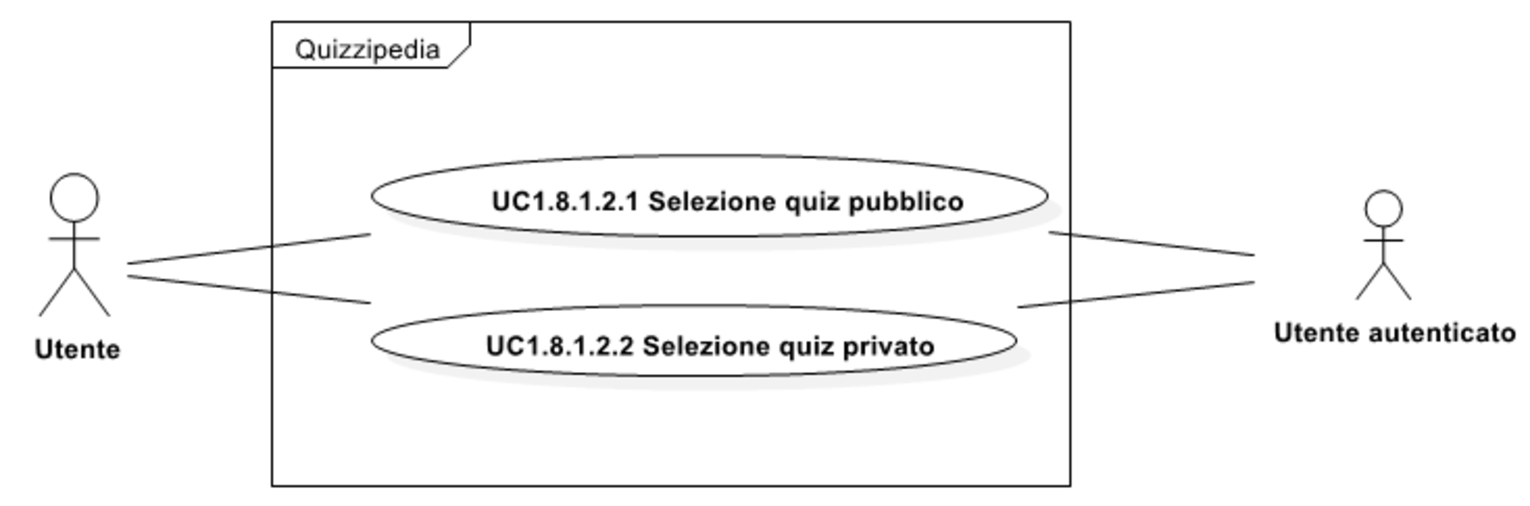
\includegraphics[width=\textwidth]{Img/UC Selezione solo quiz.pdf}}
\caption{UC1.8.1.2 Selezione solo quiz}
\end{figure}
\begin{itemize}
\item \textbf{Attori}: Utente, Utente Autenticato.
\item \textbf{Scenario principale}:
\begin{enumerate}
\item Selezione quiz pubblico (UC1.8.1.2.1);
\item Selezione quiz privato (UC1.8.1.2.2).
\end{enumerate}
\item \textbf{Descrizione}: l'utente deve poter selezionare/deselezionare l'opzione 'solo quiz', che escluderà le domande dalla ricerca. Se l'opzione 'solo domande' è stata selezionata in precedenza, sarà deselezionata automaticamente.
\item \textbf{Precondizione}: l'utente ha scelto di personalizzare la ricerca attraverso dei parametri.
\item \textbf{Postcondizione}: l'utente ha selezionato/deselezionato il parametro 'solo quiz'.
\end{itemize}
\subsubsection{UC1.8.1.2.1 Selezione quiz pubblico}
\begin{itemize}
\item \textbf{Attori}: Utente, Utente Autenticato.
\item \textbf{Descrizione}: l'utente deve poter selezionare/deselezionare l'opzione 'quiz pubblico', che escluderà dalla ricerca i quiz privati.
\item \textbf{Precondizione}: l'utente ha scelto di personalizzare la ricerca attraverso dei parametri.
\item \textbf{Postcondizione}: l'utente ha selezionato/deselezionato il parametro 'quiz pubblico'.
\end{itemize}
\subsubsection{UC1.8.1.2.2 Selezione quiz privato}
\begin{itemize}
\item \textbf{Attori}: Utente, Utente Autenticato.
\item \textbf{Scenario alternativo}: l'utente non ha il permesso di visualizzare quiz privati e non potrà selezionare l'opzione.
\item \textbf{Descrizione}: l'utente deve poter selezionare/deselezionare l'opzione 'quiz privato', che escluderà dalla ricerca i quiz privati.
\item \textbf{Precondizione}: l'utente ha scelto di personalizzare la ricerca attraverso dei parametri.
\item \textbf{Postcondizione}: l'utente ha selezionato/deselezionato il parametro 'quiz pubblico'.
\end{itemize}
\subsubsection{UC1.8.1.3 Selezione argomenti nella ricerca}
\begin{itemize}
\item \textbf{Attori}: Utente, Utente Autenticato.
\item \textbf{Descrizione}: l'utente deve poter selezionare/deselezionare uno o più argomenti, escludendo domande e quiz di argomenti non selezionati dalla ricerca.
\item \textbf{Precondizione}: l'utente ha scelto di personalizzare la ricerca attraverso dei parametri.
\item \textbf{Postcondizione}: l'utente ha selezionato/deselezionato gli argomenti.
\end{itemize}
\subsubsection{UC1.8.1.4 Selezione livelli di difficoltà}
\begin{itemize}
\item \textbf{Attori}: Utente, Utente Autenticato.
\item \textbf{Descrizione}: l'utente deve poter selezionare/deselezionare uno o più livelli di difficoltà, escludendo domande e quiz di livello di difficoltà non selezionato.
\item \textbf{Precondizione}: l'utente ha scelto di personalizzare la ricerca attraverso dei parametri.
\item \textbf{Postcondizione}: l'utente ha selezionato/deselezionato i livelli di difficoltà.
\end{itemize}
\subsubsection{UC1.8.1.5 Selezione parole chiave}
\begin{itemize}
\item \textbf{Attori}: Utente, Utente Autenticato.
\item \textbf{Descrizione}: l'utente deve poter selezionare/deselezionare uno o più parole chiave, escludendo domande e quiz in cui le parole chiave immesse non compaiono nel titolo o nella descrizione.
\item \textbf{Precondizione}: l'utente ha scelto di personalizzare la ricerca attraverso dei parametri.
\item \textbf{Postcondizione}: l'utente ha selezionato/deselezionato le parole chiave.
\end{itemize}
\subsubsection{UC1.8.2 Conferma inizio ricerca}
\begin{itemize}
\item \textbf{Attori}: Utente, Utente Autenticato.
\item \textbf{Descrizione}: l'utente deve poter confermare l'inizio della ricerca. Se sono stati inseriti dei parametri, questi dovranno essere tenuti in considerazione.
\item \textbf{Precondizione}: l'utente ha scelto di effettuare una ricerca e selezionato eventuali parametri.
\item \textbf{Postcondizione}: l'utente ha confermato l'inizio della ricerca.
\end{itemize}
\subsubsection{UC1.8.3 Visualizzazione lista risultati}
\begin{itemize}
\item \textbf{Attori}: Utente, Utente Autenticato.
\item \textbf{Descrizione}: l'utente deve poter visualizzare la lista dei risultati prodotti dalla ricerca effettuata.
\item \textbf{Precondizione}: l'utente ha scelto di effettuare una ricerca, selezionato eventuali parametri e confermato l'avvio della ricerca.
\item \textbf{Postcondizione}: l'utente ha visualizzato i risultati prodotti dalla ricerca effettuata.
\end{itemize}
\subsubsection{UC2 Caso d'uso privato}
\begin{figure}[H]
\centering
\noindent\makebox[\textwidth]{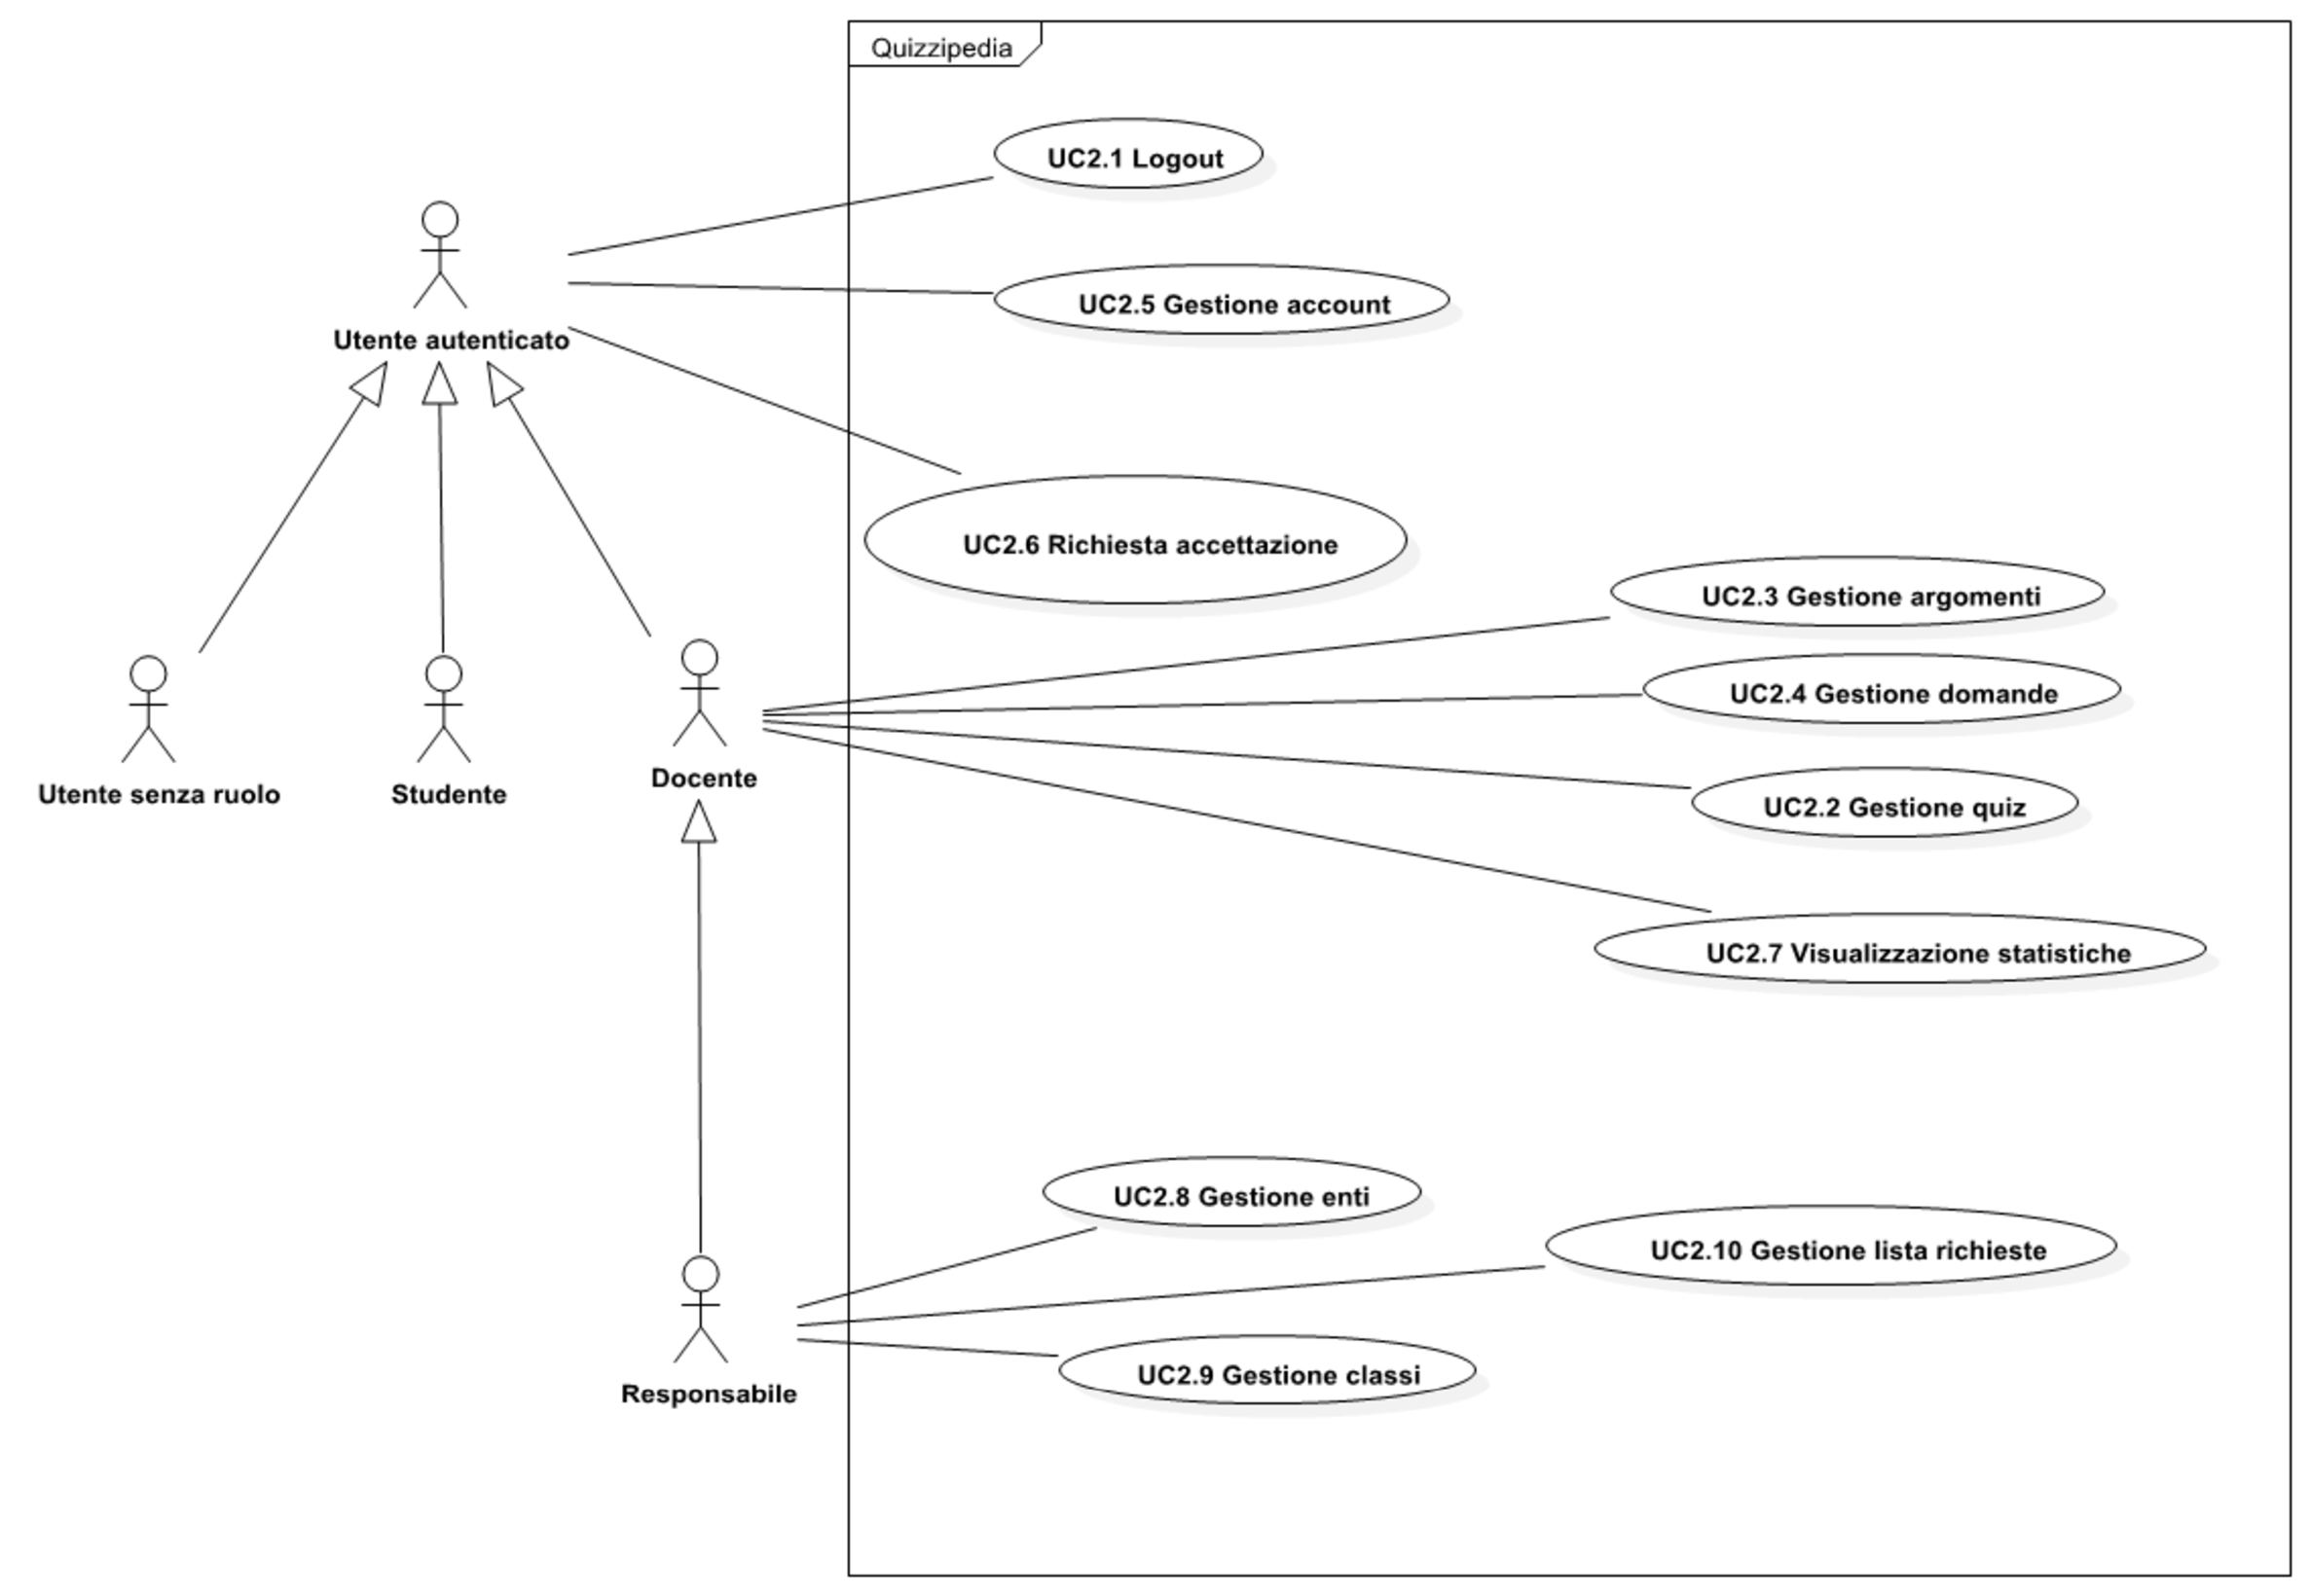
\includegraphics[width=\textwidth]{Img/UC Caso d'uso privato.pdf}}
\caption{UC2 Caso d'uso privato}
\end{figure}
\begin{itemize}
\item \textbf{Attori}: Utente Autenticato.
\item \textbf{Scenario principale}:
\begin{enumerate}
\item Logout (UC2.1);
\item Gestione quiz (UC2.2);
\item Gestione argomenti (UC2.3);
\item Gestione domande (UC2.4);
\item Gestione account (UC2.5);
\item Richiesta accettazione (UC2.6);
\item Visualizzazione statistiche (UC2.7);
\item Gestione enti (UC2.8);
\item Gestione classe (UC2.9);
\item Lista richieste (UC2.10).
\end{enumerate}
\item \textbf{Descrizione}: l'utente autenticato può accedere ad aree private a seconda dei permessi di cui dispone.
\item \textbf{Precondizione}: l'utente è in possesso di un account Quizzipedia e si è precedentemente autenticato.
\item \textbf{Postcondizione}: l'utente ha scelto l'operazione da intraprendere.
\end{itemize}
\subsubsection{UC2.1 Logout}
\begin{itemize}
\item \textbf{Attori}: Utente Autenticato.
\item \textbf{Descrizione}: l'utente può effettuare il logout dall'area privata.
\item \textbf{Precondizione}: l'utente è in possesso di un account Quizzipedia e si è precedentemente autenticato.
\item \textbf{Postcondizione}: l'utente ha effettuato il logout e ora non è più autenticato.
\end{itemize}
\subsubsection{UC2.2 Gestione quiz}
\begin{figure}[H]
\centering
\noindent\makebox[\textwidth]{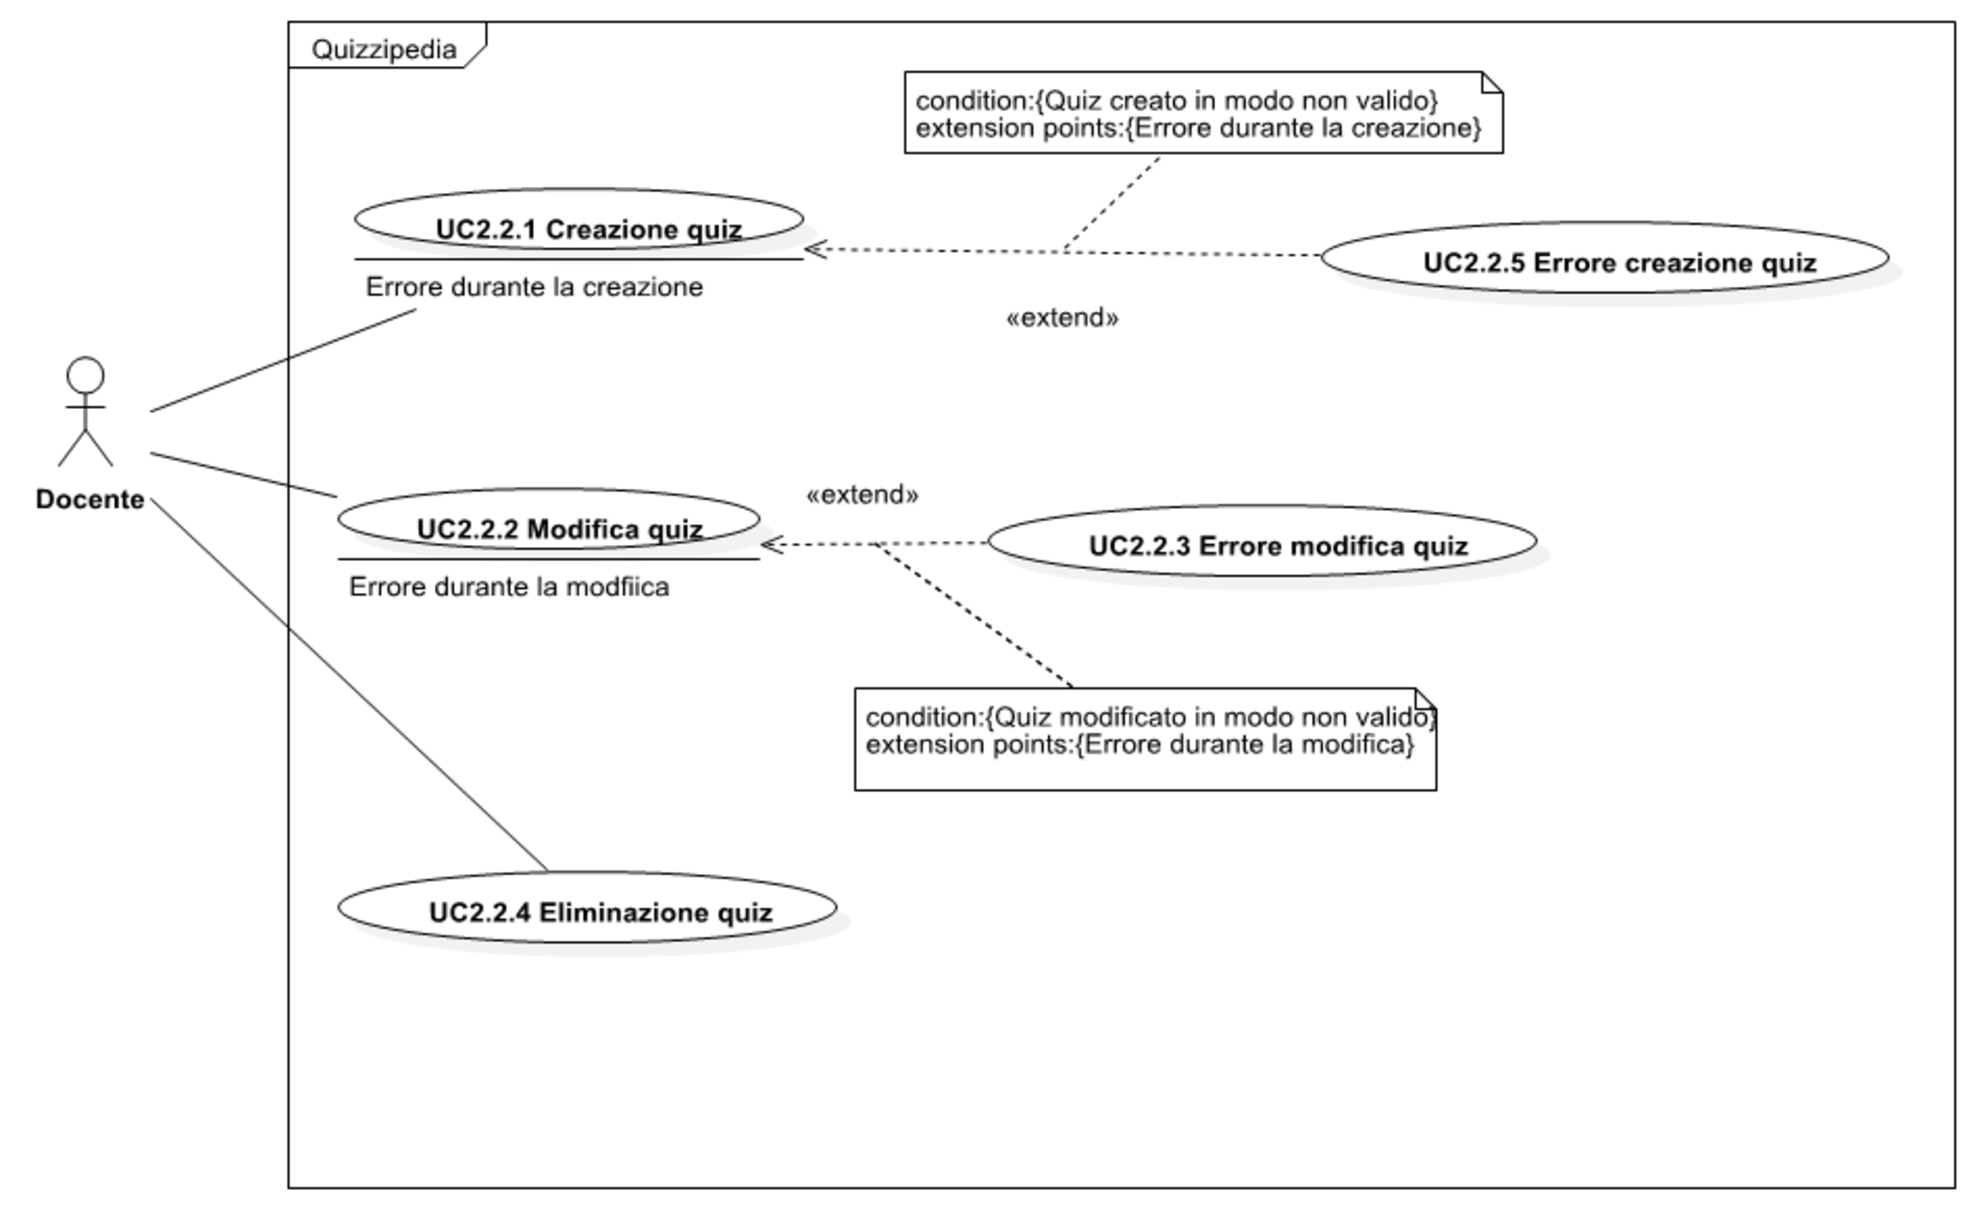
\includegraphics[width=\textwidth]{Img/UC Gestione quiz.pdf}}
\caption{UC2.2 Gestione quiz}
\end{figure}
\begin{itemize}
\item \textbf{Attori}: Docente.
\item \textbf{Scenario principale}:
\begin{enumerate}
\item Creazione quiz (UC2.2.1);
\item Modifica quiz (UC2.2.2);
\item Errore durante la modifica del quiz (UC2.2.3);
\item Eliminazione quiz (UC2.2.4).
\end{enumerate}
\item \textbf{Descrizione}: il docente deve poter effettuare varie operazioni di gestione di quiz, in particolare deve poter creare quiz nuovi e modificare o eliminare quiz esistenti.
\item \textbf{Precondizione}: il docente è autenticato nel sistema e desidera effettuare operazioni sui quiz.
\item \textbf{Postcondizione}: il docente ha effettuato le operazioni desiderate sui quiz.
\end{itemize}
\subsubsection{UC2.2.1 Creazione quiz}
\begin{figure}[H]
\centering
\noindent\makebox[\textwidth]{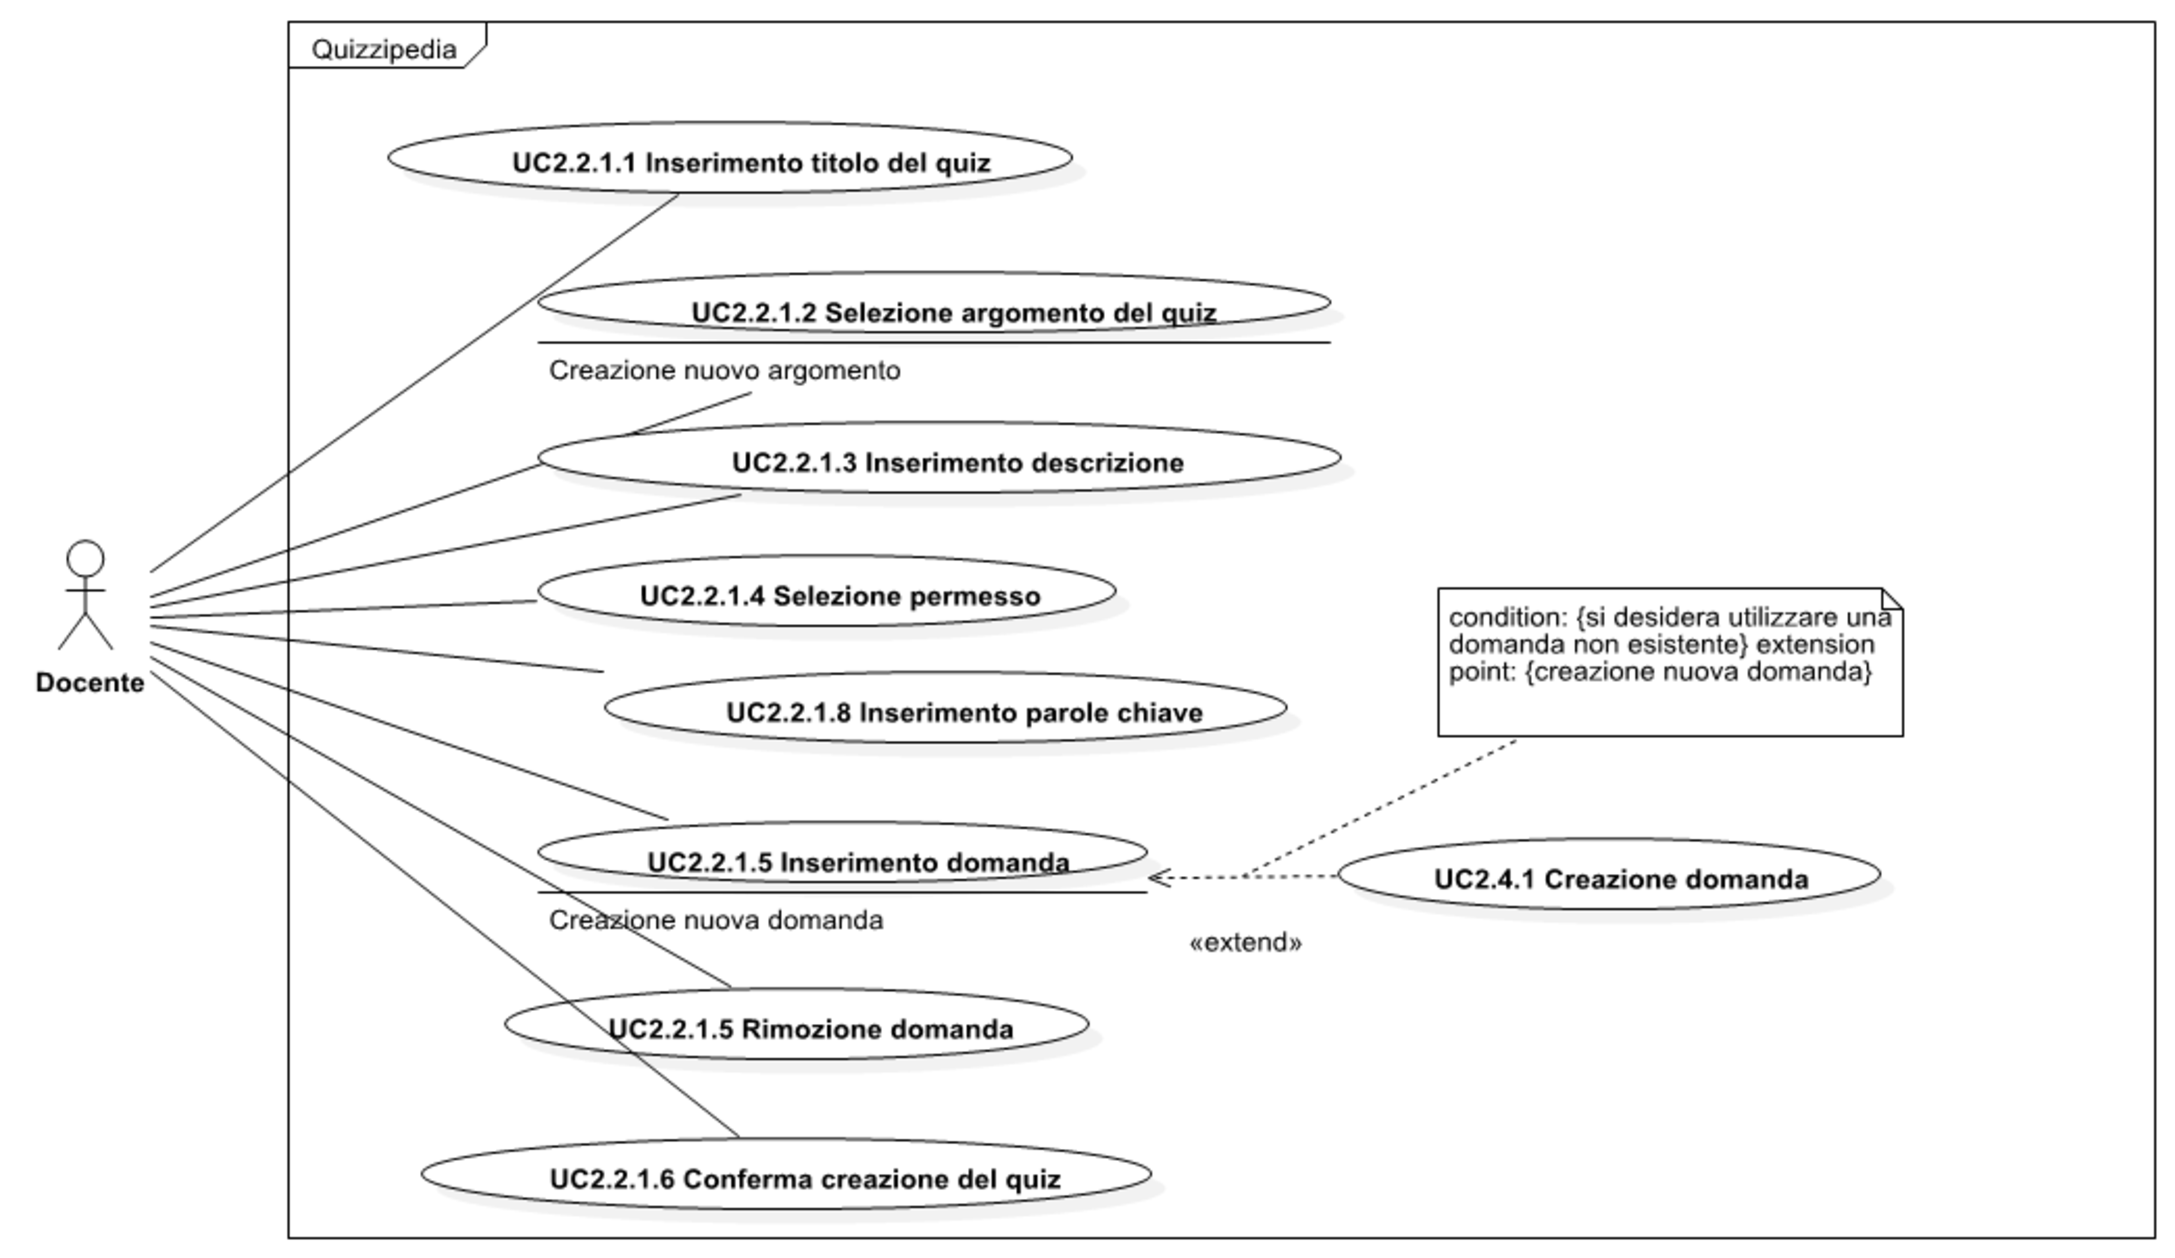
\includegraphics[width=\textwidth]{Img/UC Creazione quiz.pdf}}
\caption{UC2.2.1 Creazione quiz}
\end{figure}
\begin{itemize}
\item \textbf{Attori}: Docente.
\item \textbf{Scenario principale}:
\begin{enumerate}
\item Inserimento titolo (UC2.2.1.1);
\item Selezione argomento del quiz (UC2.2.1.2);
\item Inserimento descrizione (UC2.2.1.3);
\item Conferma creazione quiz (UC2.2.1.4).
\end{enumerate}
\item \textbf{Scenario alternativo}: il docente interrompe la creazione del quiz.
\item \textbf{Inclusioni}:
\begin{itemize}
\item Modifica quiz (UC2.2.2).
\end{itemize}
\item \textbf{Descrizione}: il docente deve poter creare un nuovo quiz.
\item \textbf{Precondizione}: il docente è autenticato nel sistema e desidera creare un nuovo quiz.
\item \textbf{Postcondizione}: il docente ha creato il nuovo quiz.
\end{itemize}
\subsubsection{UC2.2.1.1 Inserimento titolo}
\begin{itemize}
\item \textbf{Attori}: Docente.
\item \textbf{Descrizione}: il docente deve poter inserire il titolo del quiz che sta creando.
\item \textbf{Precondizione}: il docente sta creando un nuovo quiz e deve ancora inserire il titolo.
\item \textbf{Postcondizione}: il docente ha inserito il titolo del quiz.
\end{itemize}
\subsubsection{UC2.2.1.2 Selezione argomento del quiz}
\begin{itemize}
\item \textbf{Attori}: Docente.
\item \textbf{Estensioni}:
\begin{itemize}
\item Creazione argomento (UC2.3.1).
\end{itemize}
\item \textbf{Descrizione}: il docente deve poter selezionare l'argomento del quiz da una lista di argomenti, o creare un nuovo argomento se è mancante.
\item \textbf{Precondizione}: il docente sta creando un nuovo quiz e deve selezionare l'argomento.
\item \textbf{Postcondizione}: il docente ha selezionato l'argomento del quiz.
\end{itemize}
\subsubsection{UC2.2.1.3 Inserimento descrizione}
\begin{itemize}
\item \textbf{Attori}: Docente.
\item \textbf{Descrizione}: il docente deve poter inserire la descrizione del quiz che sta creando.
\item \textbf{Precondizione}: il docente sta creando un nuovo quiz e deve ancora inserire la descrizione.
\item \textbf{Postcondizione}: il docente ha inserito la descrizione del quiz.
\end{itemize}
\subsubsection{UC2.2.1.4 Conferma creazione quiz}
\begin{itemize}
\item \textbf{Attori}: Docente.
\item \textbf{Descrizione}: il docente deve confermare la creazione del nuovo quiz per portarla a termine.
\item \textbf{Precondizione}: il docente sta creando un nuovo quiz e deve ancora confermare la sua creazione.
\item \textbf{Postcondizione}: il docente ha confermato la creazione del quiz.
\end{itemize}
\subsubsection{UC2.2.2 Modifica quiz}
\begin{figure}[H]
\centering
\noindent\makebox[\textwidth]{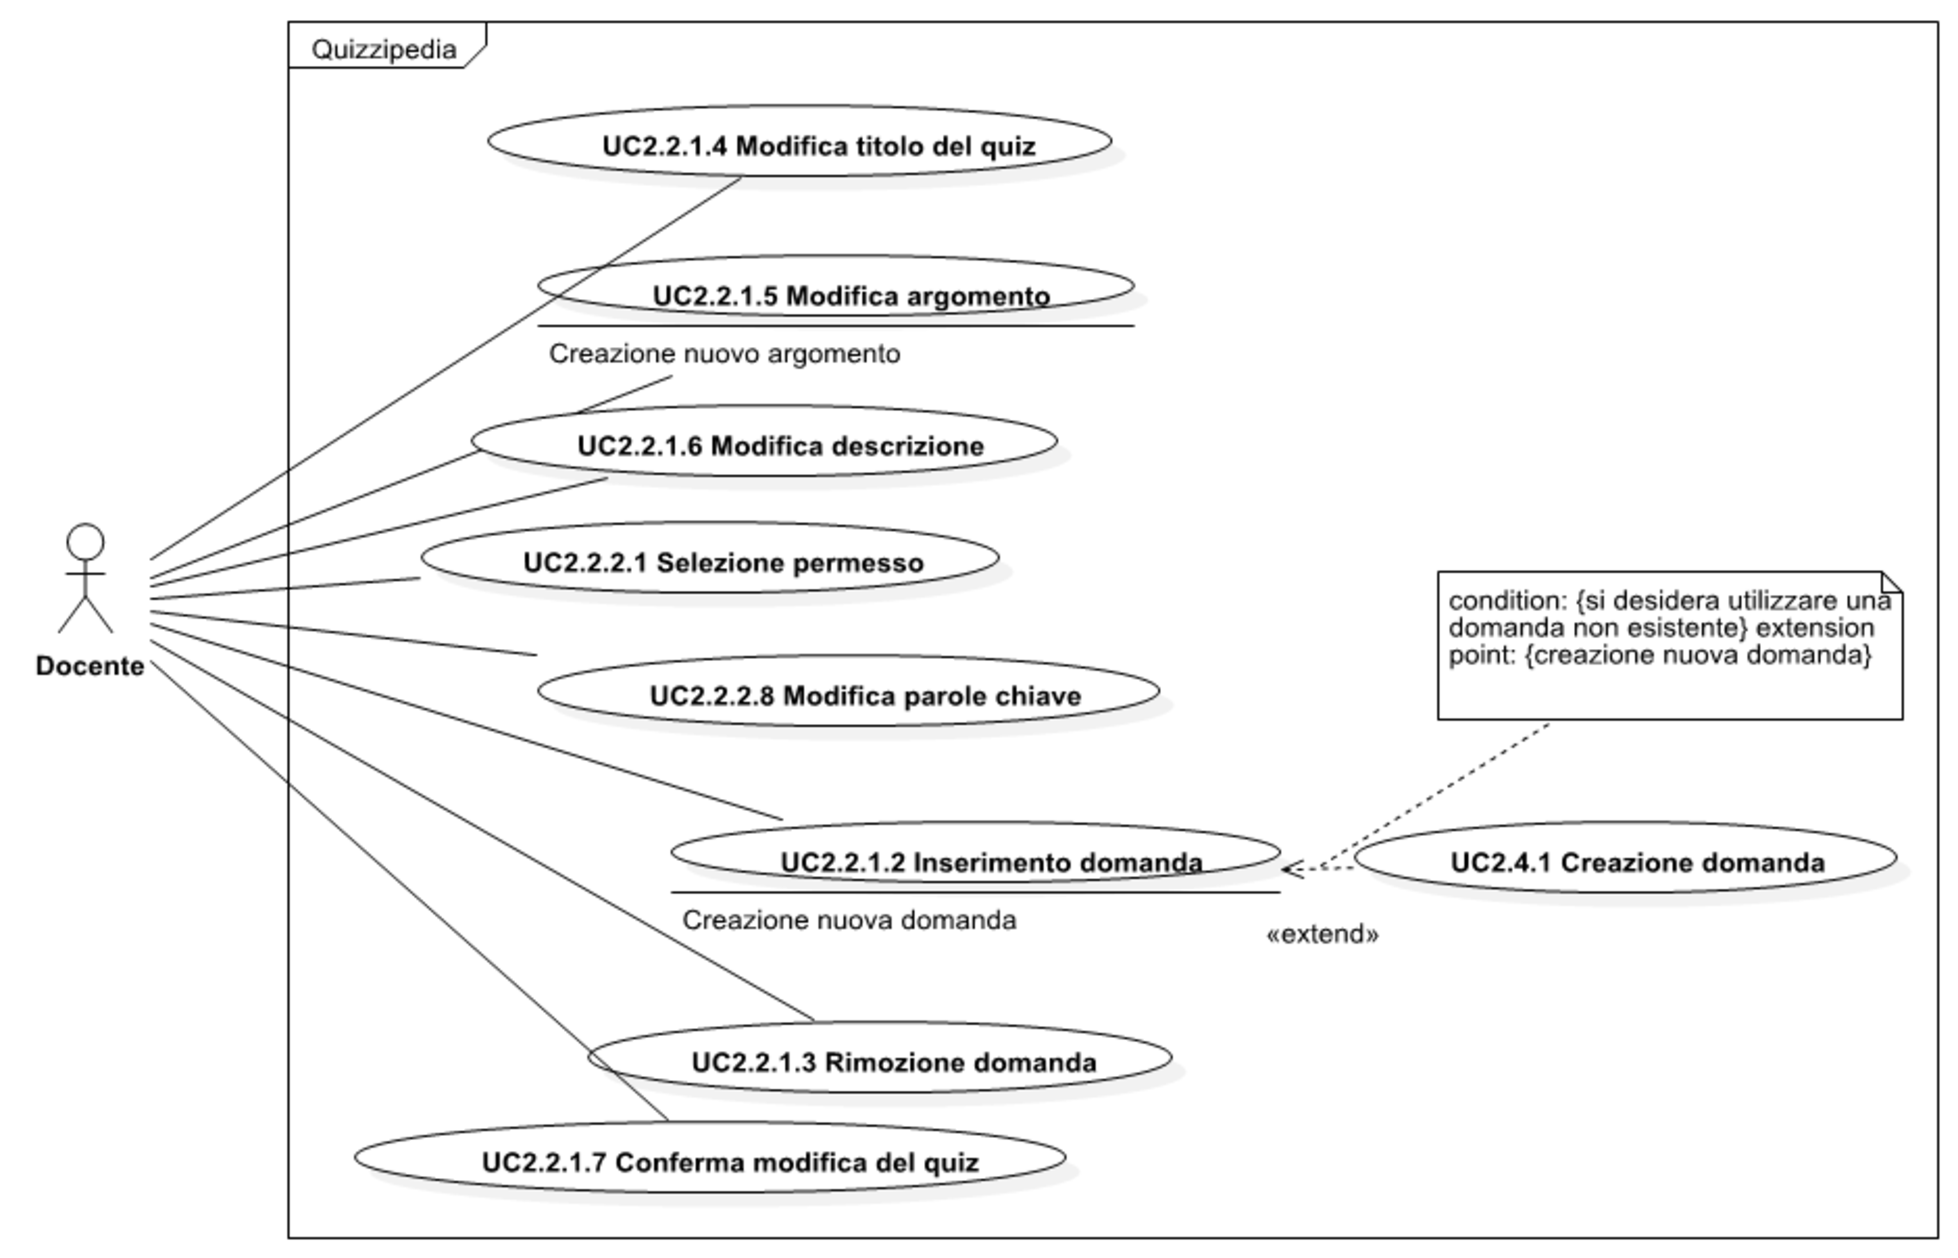
\includegraphics[width=\textwidth]{Img/UC Modifica quiz.pdf}}
\caption{UC2.2.2 Modifica quiz}
\end{figure}
\begin{itemize}
\item \textbf{Attori}: Docente.
\item \textbf{Scenario principale}:
\begin{enumerate}
\item Selezione permesso (UC2.2.2.1);
\item Inserimento domanda nel quiz (UC2.2.2.2);
\item Rimozione domanda dal quiz (UC2.2.2.3);
\item Modifica titolo (UC2.2.2.4);
\item Modifica argomento (UC2.2.2.5);
\item Modifica descrizione (UC2.2.2.6);
\item Conferma modifica quiz (UC2.2.2.7).
\end{enumerate}
\item \textbf{Estensioni}:
\begin{itemize}
\item Errore durante la modifica del quiz (UC2.2.3);
\item Creazione domanda (UC2.4.1).
\end{itemize}
\item \textbf{Descrizione}: il docente deve poter modificare un quiz.
\item \textbf{Precondizione}: il docente è autenticato nel sistema e desidera modificare un quiz.
\item \textbf{Postcondizione}: il docente ha modificato il quiz.
\end{itemize}
\subsubsection{UC2.2.2.1 Selezione permesso}
\begin{figure}[H]
\centering
\noindent\makebox[\textwidth]{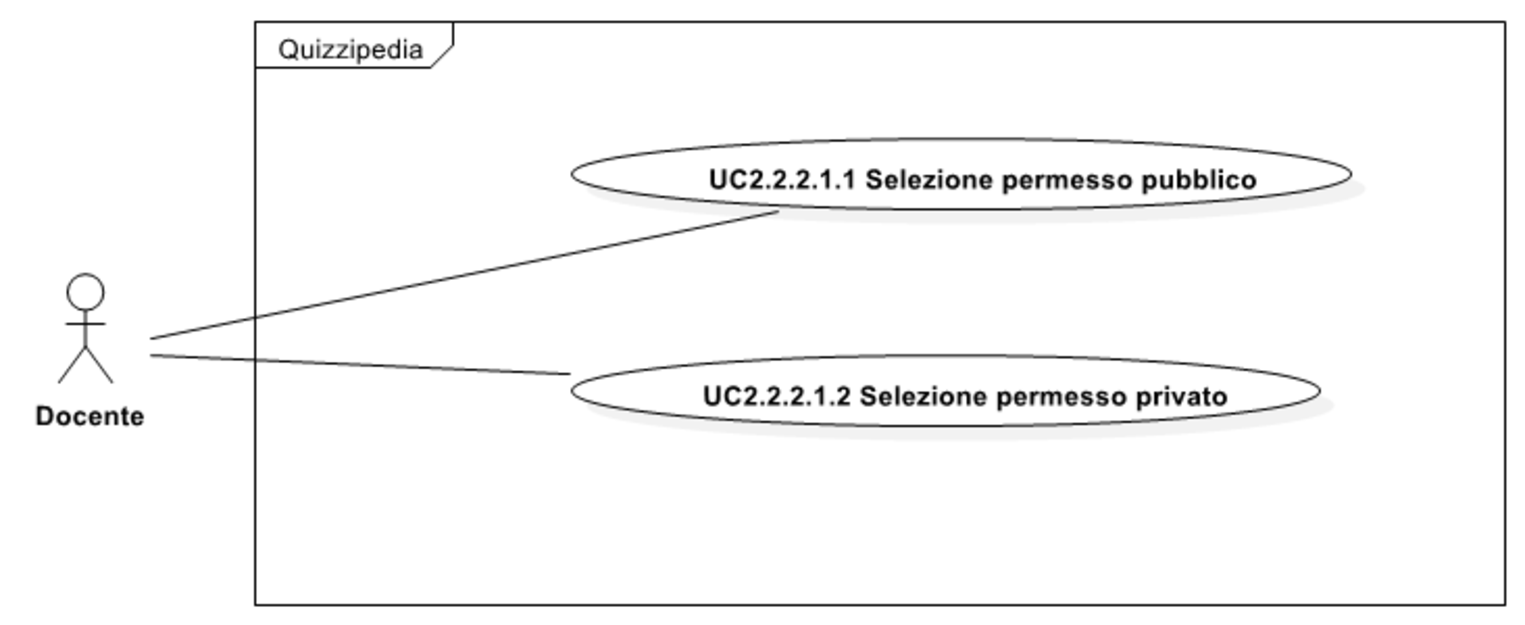
\includegraphics[width=\textwidth]{Img/UC Selezione permesso.pdf}}
\caption{UC2.2.2.1 Selezione permesso}
\end{figure}
\begin{itemize}
\item \textbf{Attori}: Docente.
\item \textbf{Scenario principale}:
\begin{enumerate}
\item Selezione permesso pubblico (UC2.2.2.1.1);
\item Selezione permesso privato (UC2.2.2.1.2).
\end{enumerate}
\item \textbf{Descrizione}: il docente deve poter scegliere il permesso del quiz.
\item \textbf{Precondizione}: il docente sta modificando un quiz.
\item \textbf{Postcondizione}: il docente ha specificato il permesso del quiz.
\end{itemize}
\subsubsection{UC2.2.2.1.1 Selezione permesso pubblico}
\begin{itemize}
\item \textbf{Attori}: Responsabile.
\item \textbf{Descrizione}: il docente ha scelto un permesso 'pubblico' per il quiz, permettendo a tutti gli utenti di svolgerlo senza restrizioni.
\item \textbf{Precondizione}: il docente sta selezionando il permesso di un quiz.
\item \textbf{Postcondizione}: il docente ha scelto il permesso 'pubblico'.
\end{itemize}
\subsubsection{UC2.2.2.1.2 Selezione permesso privato}
\begin{figure}[H]
\centering
\noindent\makebox[\textwidth]{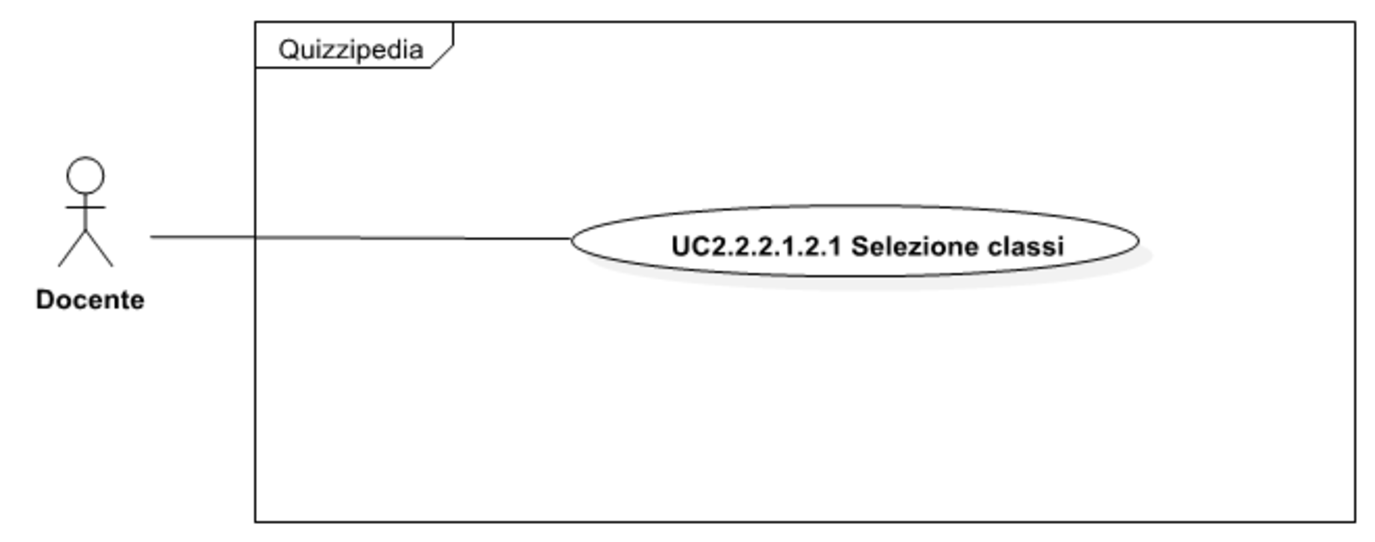
\includegraphics[width=\textwidth]{Img/UC Selezione permesso privato.pdf}}
\caption{UC2.2.2.1.2 Selezione permesso privato}
\end{figure}
\begin{itemize}
\item \textbf{Attori}: Docente.
\item \textbf{Scenario principale}:
\begin{enumerate}
\item Selezione classi (UC2.2.2.1.2.1).
\end{enumerate}
\item \textbf{Descrizione}: il docente ha scelto un permesso privato per il quiz, limitando il suo accesso e svolgimento a una cerchia ristretta di studenti.
\item \textbf{Precondizione}: il docente sta selezionando il permesso di un quiz.
\item \textbf{Postcondizione}: il docente ha scelto il permesso privato.
\end{itemize}
\subsubsection{UC2.2.2.1.2.1 Selezione classi}
\begin{itemize}
\item \textbf{Attori}: Docente.
\item \textbf{Descrizione}: il docente può assegnare il quiz privato a una o più classi di studenti, i cui partecipanti avranno diritto di svolgerlo.
\item \textbf{Precondizione}: il docente ha selezionato un permesso 'privato' per il quiz.
\item \textbf{Postcondizione}: il docente ha selezionato le classi a cui assegnare il quiz.
\end{itemize}
\subsubsection{UC2.2.2.2 Inserimento domanda nel quiz}
\begin{itemize}
\item \textbf{Attori}: Docente.
\item \textbf{Estensioni}:
\begin{itemize}
\item Ricerca quiz e domande (UC1.8).
\end{itemize}
\item \textbf{Descrizione}: il docente deve poter inserire una domanda nel quiz.
\item \textbf{Precondizione}: il docente sta modificando un quiz e vuole inserire una domanda.
\item \textbf{Postcondizione}: il docente ha inserito la domanda.
\end{itemize}
\subsubsection{UC2.2.2.3 Rimozione domanda dal quiz}
\begin{itemize}
\item \textbf{Attori}: Docente.
\item \textbf{Descrizione}: il docente deve poter rimuovere una domanda nel quiz (la domanda non sarà cancellata ma soltanto rimossa dal quiz).
\item \textbf{Precondizione}: il docente sta modificando il quiz e vuole rimuovere una domanda.
\item \textbf{Postcondizione}: il docente ha rimosso la domanda.
\end{itemize}
\subsubsection{UC2.2.2.4 Modifica titolo}
\begin{itemize}
\item \textbf{Attori}: Docente.
\item \textbf{Descrizione}: il docente deve poter modificare il titolo del quiz.
\item \textbf{Precondizione}: il docente sta modificando un nuovo quiz.
\item \textbf{Postcondizione}: il docente ha modificato il titolo del quiz.
\end{itemize}
\subsubsection{UC2.2.2.5 Modifica argomento}
\begin{figure}[H]
\centering
\noindent\makebox[\textwidth]{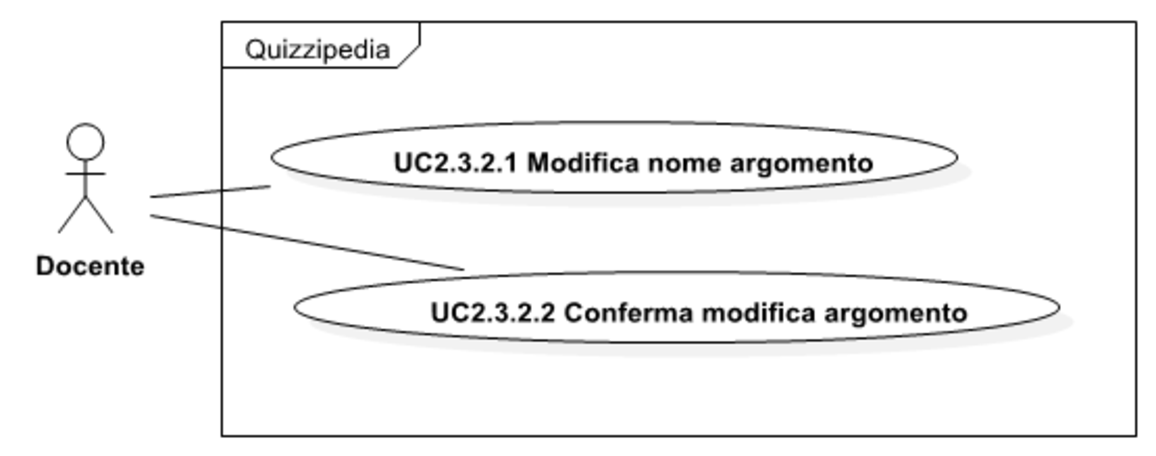
\includegraphics[width=\textwidth]{Img/UC Modifica argomento.pdf}}
\caption{UC2.2.2.5 Modifica argomento}
\end{figure}
\begin{itemize}
\item \textbf{Attori}: Docente.
\item \textbf{Estensioni}:
\begin{itemize}
\item Creazione argomento (UC2.3.1).
\end{itemize}
\item \textbf{Descrizione}: il docente deve poter selezionare l'argomento del quiz da una lista di argomenti, o creare un nuovo argomento se è mancante.
\item \textbf{Precondizione}: il docente sta modificando un quiz.
\item \textbf{Postcondizione}: il docente ha modificato l'argomento del quiz.
\end{itemize}
\subsubsection{UC2.2.2.6 Modifica descrizione}
\begin{itemize}
\item \textbf{Attori}: Docente.
\item \textbf{Descrizione}: il docente deve poter modificare la descrizione del quiz.
\item \textbf{Precondizione}: il docente sta modificando un quiz.
\item \textbf{Postcondizione}: il docente ha modificato la descrizione del quiz.
\end{itemize}
\subsubsection{UC2.2.2.7 Conferma modifica quiz}
\begin{itemize}
\item \textbf{Attori}: Docente.
\item \textbf{Descrizione}: il docente deve confermare la modifica del quiz per portarla a termine.
\item \textbf{Precondizione}: il docente sta modificando un quiz e deve ancora confermare la sua modifica.
\item \textbf{Postcondizione}: il docente ha confermato la modifica del quiz.
\end{itemize}
\subsubsection{UC2.2.3 Errore durante la modifica del quiz}
\begin{itemize}
\item \textbf{Attori}: Docente.
\item \textbf{Descrizione}: si è verificata la seguente condizione: il numero di risposte selezionate è eccessivo o pari a zero.
\item \textbf{Precondizione}: il docente ha iniziato una modifica del quiz che non è andata a buon termine.
\item \textbf{Postcondizione}: il docente ha visualizzato l'errore.
\end{itemize}
\subsubsection{UC2.2.4 Eliminazione quiz}
\begin{figure}[H]
\centering
\noindent\makebox[\textwidth]{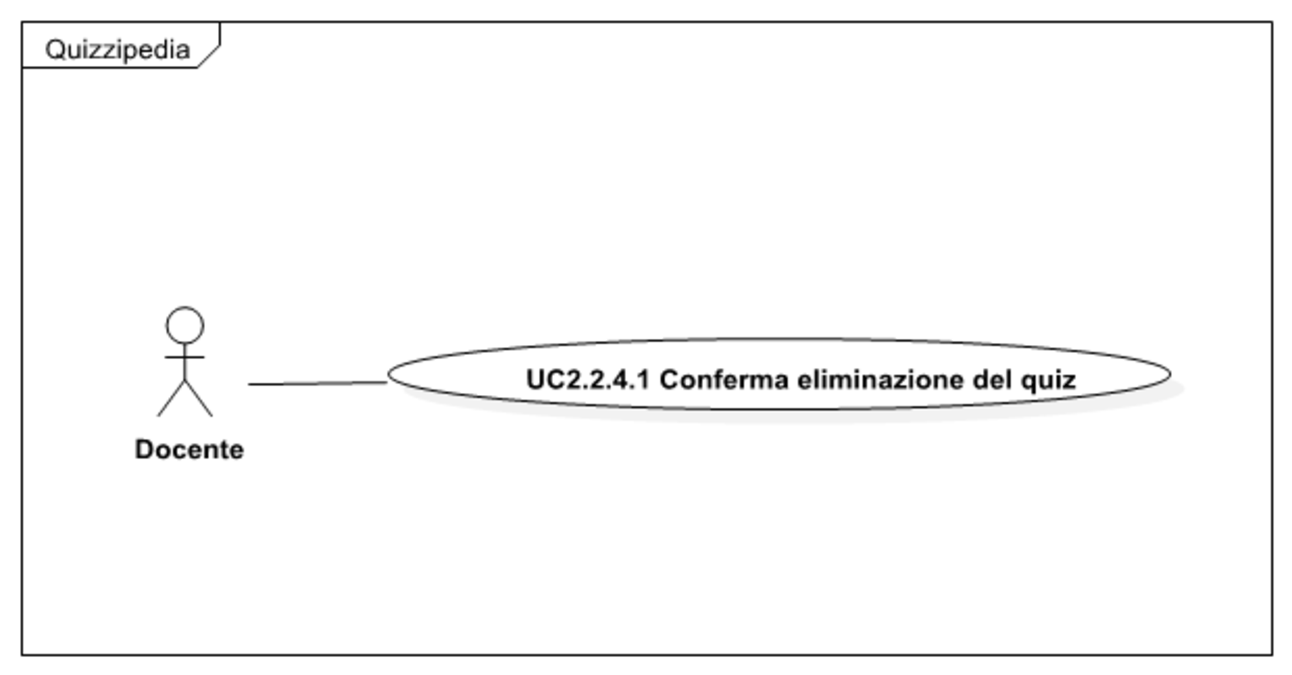
\includegraphics[width=\textwidth]{Img/UC Eliminazione quiz.pdf}}
\caption{UC2.2.4 Eliminazione quiz}
\end{figure}
\begin{itemize}
\item \textbf{Attori}: Docente.
\item \textbf{Scenario principale}:
\begin{enumerate}
\item conferma eliminazione del quiz (UC2.2.4.1).
\end{enumerate}
\item \textbf{Descrizione}: il docente deve poter eliminare un quiz. Questo non causerà l'eliminazione delle domande contenute nel quiz.
\item \textbf{Precondizione}: il docente è autenticato nel sistema e desidera eliminare un quiz esistente.
\item \textbf{Postcondizione}: il docente ha eliminato il quiz.
\end{itemize}
\subsubsection{UC2.2.4.1 conferma eliminazione del quiz}
\begin{itemize}
\item \textbf{Attori}: Docente.
\item \textbf{Descrizione}: il docente dovrà confermare l'eliminazione del quiz.
\item \textbf{Precondizione}: il docente ha richiesto l'eliminazione di un quiz e deve ancora effettuare la conferma.
\item \textbf{Postcondizione}: il docente ha confermato l'eliminazione del quiz.
\end{itemize}
\subsubsection{UC2.3 Gestione argomenti}
\begin{figure}[H]
\centering
\noindent\makebox[\textwidth]{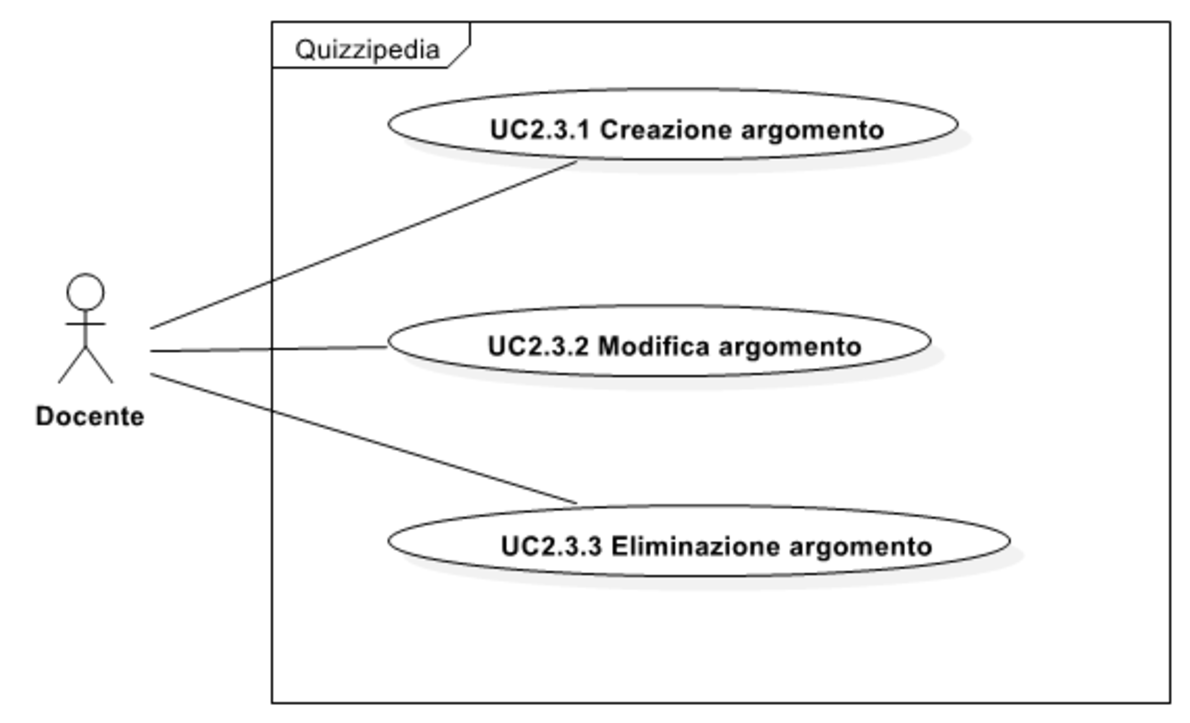
\includegraphics[width=\textwidth]{Img/UC Gestione argomenti.pdf}}
\caption{UC2.3 Gestione argomenti}
\end{figure}
\begin{itemize}
\item \textbf{Attori}: Docente.
\item \textbf{Scenario principale}:
\begin{enumerate}
\item Creazione argomento (UC2.3.1);
\item Modifica argomento (UC2.3.2);
\item Rimozione argomento (UC2.3.3).
\end{enumerate}
\item \textbf{Descrizione}: il docente deve poter gestire gli argomenti di quiz e domande, in particolare può inserire nuovi argomenti e modificare o eliminare argomenti esistenti.
\item \textbf{Precondizione}: il docente è autenticato e desidera effettuare operazioni sugli argomenti.
\item \textbf{Postcondizione}: il docente ha effettuato le operazioni sugli argomenti.
\end{itemize}
\subsubsection{UC2.3.1 Creazione argomento}
\begin{figure}[H]
\centering
\noindent\makebox[\textwidth]{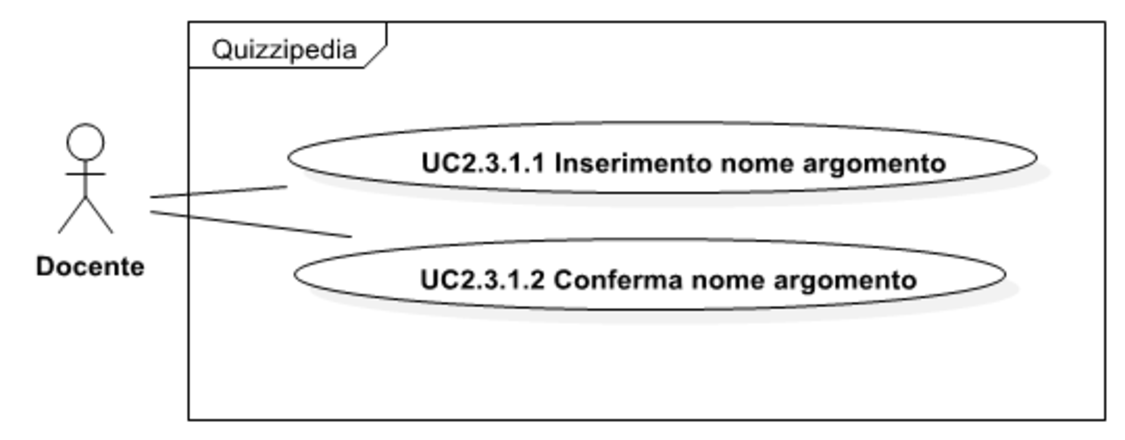
\includegraphics[width=\textwidth]{Img/UC Creazione argomento.pdf}}
\caption{UC2.3.1 Creazione argomento}
\end{figure}
\begin{itemize}
\item \textbf{Attori}: Docente.
\item \textbf{Scenario principale}:
\begin{enumerate}
\item Inserimento nome argomento (UC2.3.1.1);
\item Conferma creazione argomento (UC2.3.1.2).
\end{enumerate}
\item \textbf{Descrizione}: il docente deve poter creare un nuovo argomento.
\item \textbf{Precondizione}: il docente è autenticato e vuole creare un nuovo argomento.
\item \textbf{Postcondizione}: il docente ha creato il nuovo argomento.
\end{itemize}
\subsubsection{UC2.3.1.1 Inserimento nome argomento}
\begin{itemize}
\item \textbf{Attori}: Docente.
\item \textbf{Descrizione}: il docente deve poter inserire il nome dell'argomento.
\item \textbf{Precondizione}: il docente sta creando un nuovo argomento e deve ancora inserire il nome.
\item \textbf{Postcondizione}: il docente ha inserito il nome dell'argomento.
\end{itemize}
\subsubsection{UC2.3.1.2 Conferma creazione argomento}
\begin{itemize}
\item \textbf{Attori}: Docente.
\item \textbf{Descrizione}: il docente deve poter confermare la creazione dell'argomento.
\item \textbf{Precondizione}: il docente ha inserito un nuovo argomento e deve ancora confermare.
\item \textbf{Postcondizione}: il docente ha confermato il nuovo argomento.
\end{itemize}
\subsubsection{UC2.3.2 Modifica argomento}
\begin{figure}[H]
\centering
\noindent\makebox[\textwidth]{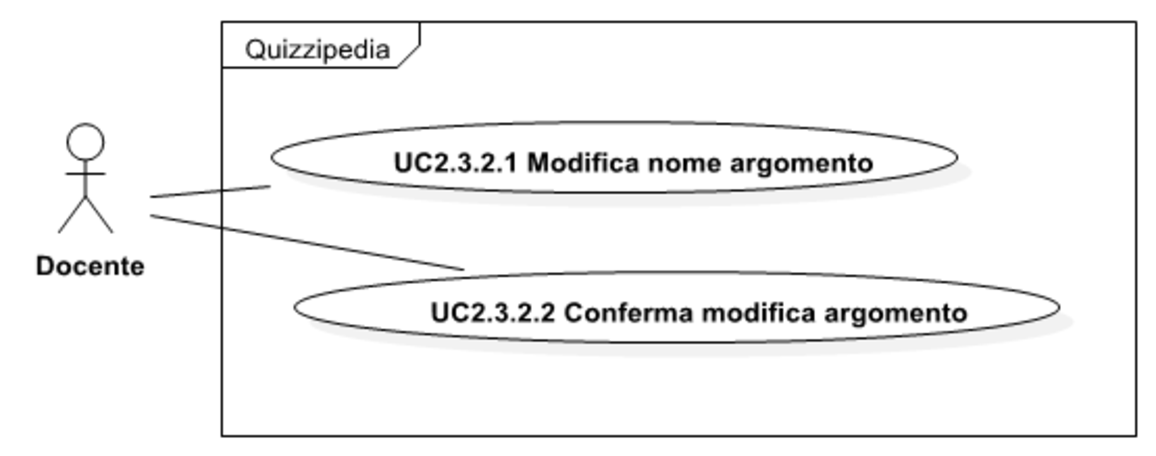
\includegraphics[width=\textwidth]{Img/UC Modifica argomento.pdf}}
\caption{UC2.3.2 Modifica argomento}
\end{figure}
\begin{itemize}
\item \textbf{Attori}: Docente.
\item \textbf{Scenario principale}:
\begin{enumerate}
\item Modifica nome argomento (UC2.3.2.1);
\item Conferma modifica argomento (UC2.3.2.2).
\end{enumerate}
\item \textbf{Descrizione}: il docente deve poter modificare un argomento.
\item \textbf{Precondizione}: il docente vuole modificare un argomento.
\item \textbf{Postcondizione}: il docente ha modificato un argomento .
\end{itemize}
\subsubsection{UC2.3.2.1 Modifica nome argomento}
\begin{itemize}
\item \textbf{Attori}: Docente.
\item \textbf{Descrizione}: il docente deve poter modificare il nome dell'argomento.
\item \textbf{Precondizione}: il docente vuole modificare il nome di un argomento.
\item \textbf{Postcondizione}: il docente ha modificato il nome di un argomento.
\end{itemize}
\subsubsection{UC2.3.2.2 Conferma modifica argomento}
\begin{itemize}
\item \textbf{Attori}: Docente.
\item \textbf{Descrizione}: il docente deve poter confermare la modifica dell'argomento.
\item \textbf{Precondizione}: il docente ha modificato un argomento e deve confermare la modifica.
\item \textbf{Postcondizione}: il docente ha confermato la modifica.
\end{itemize}
\subsubsection{UC2.3.3 Rimozione argomento}
\begin{figure}[H]
\centering
\noindent\makebox[\textwidth]{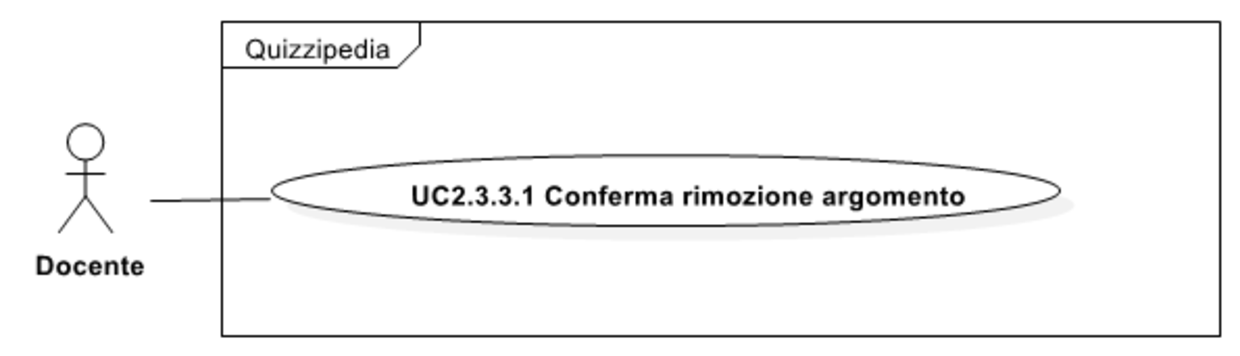
\includegraphics[width=\textwidth]{Img/UC Rimozione argomento.pdf}}
\caption{UC2.3.3 Rimozione argomento}
\end{figure}
\begin{itemize}
\item \textbf{Attori}: Docente.
\item \textbf{Scenario principale}:
\begin{enumerate}
\item Conferma rimozione argomento (UC2.3.3.1).
\end{enumerate}
\item \textbf{Descrizione}: il docente deve poter rimuovere un argomento.
\item \textbf{Precondizione}: il docente è nella gestione degli argomenti e vuole eliminare un argomento.
\item \textbf{Postcondizione}: il docente ha eliminato l'argomento.
\end{itemize}
\subsubsection{UC2.3.3.1 Conferma rimozione argomento}
\begin{itemize}
\item \textbf{Attori}: Docente.
\item \textbf{Descrizione}: il docente deve poter confermare la rimozione dell'argomento.
\item \textbf{Precondizione}: il docente ha selezionato l'argomento da eliminare e deve ancora confermare.
\item \textbf{Postcondizione}: il docente ha confermato l'argomento da eliminare.
\end{itemize}
\subsubsection{UC2.4 Gestione domande}
\begin{figure}[H]
\centering
\noindent\makebox[\textwidth]{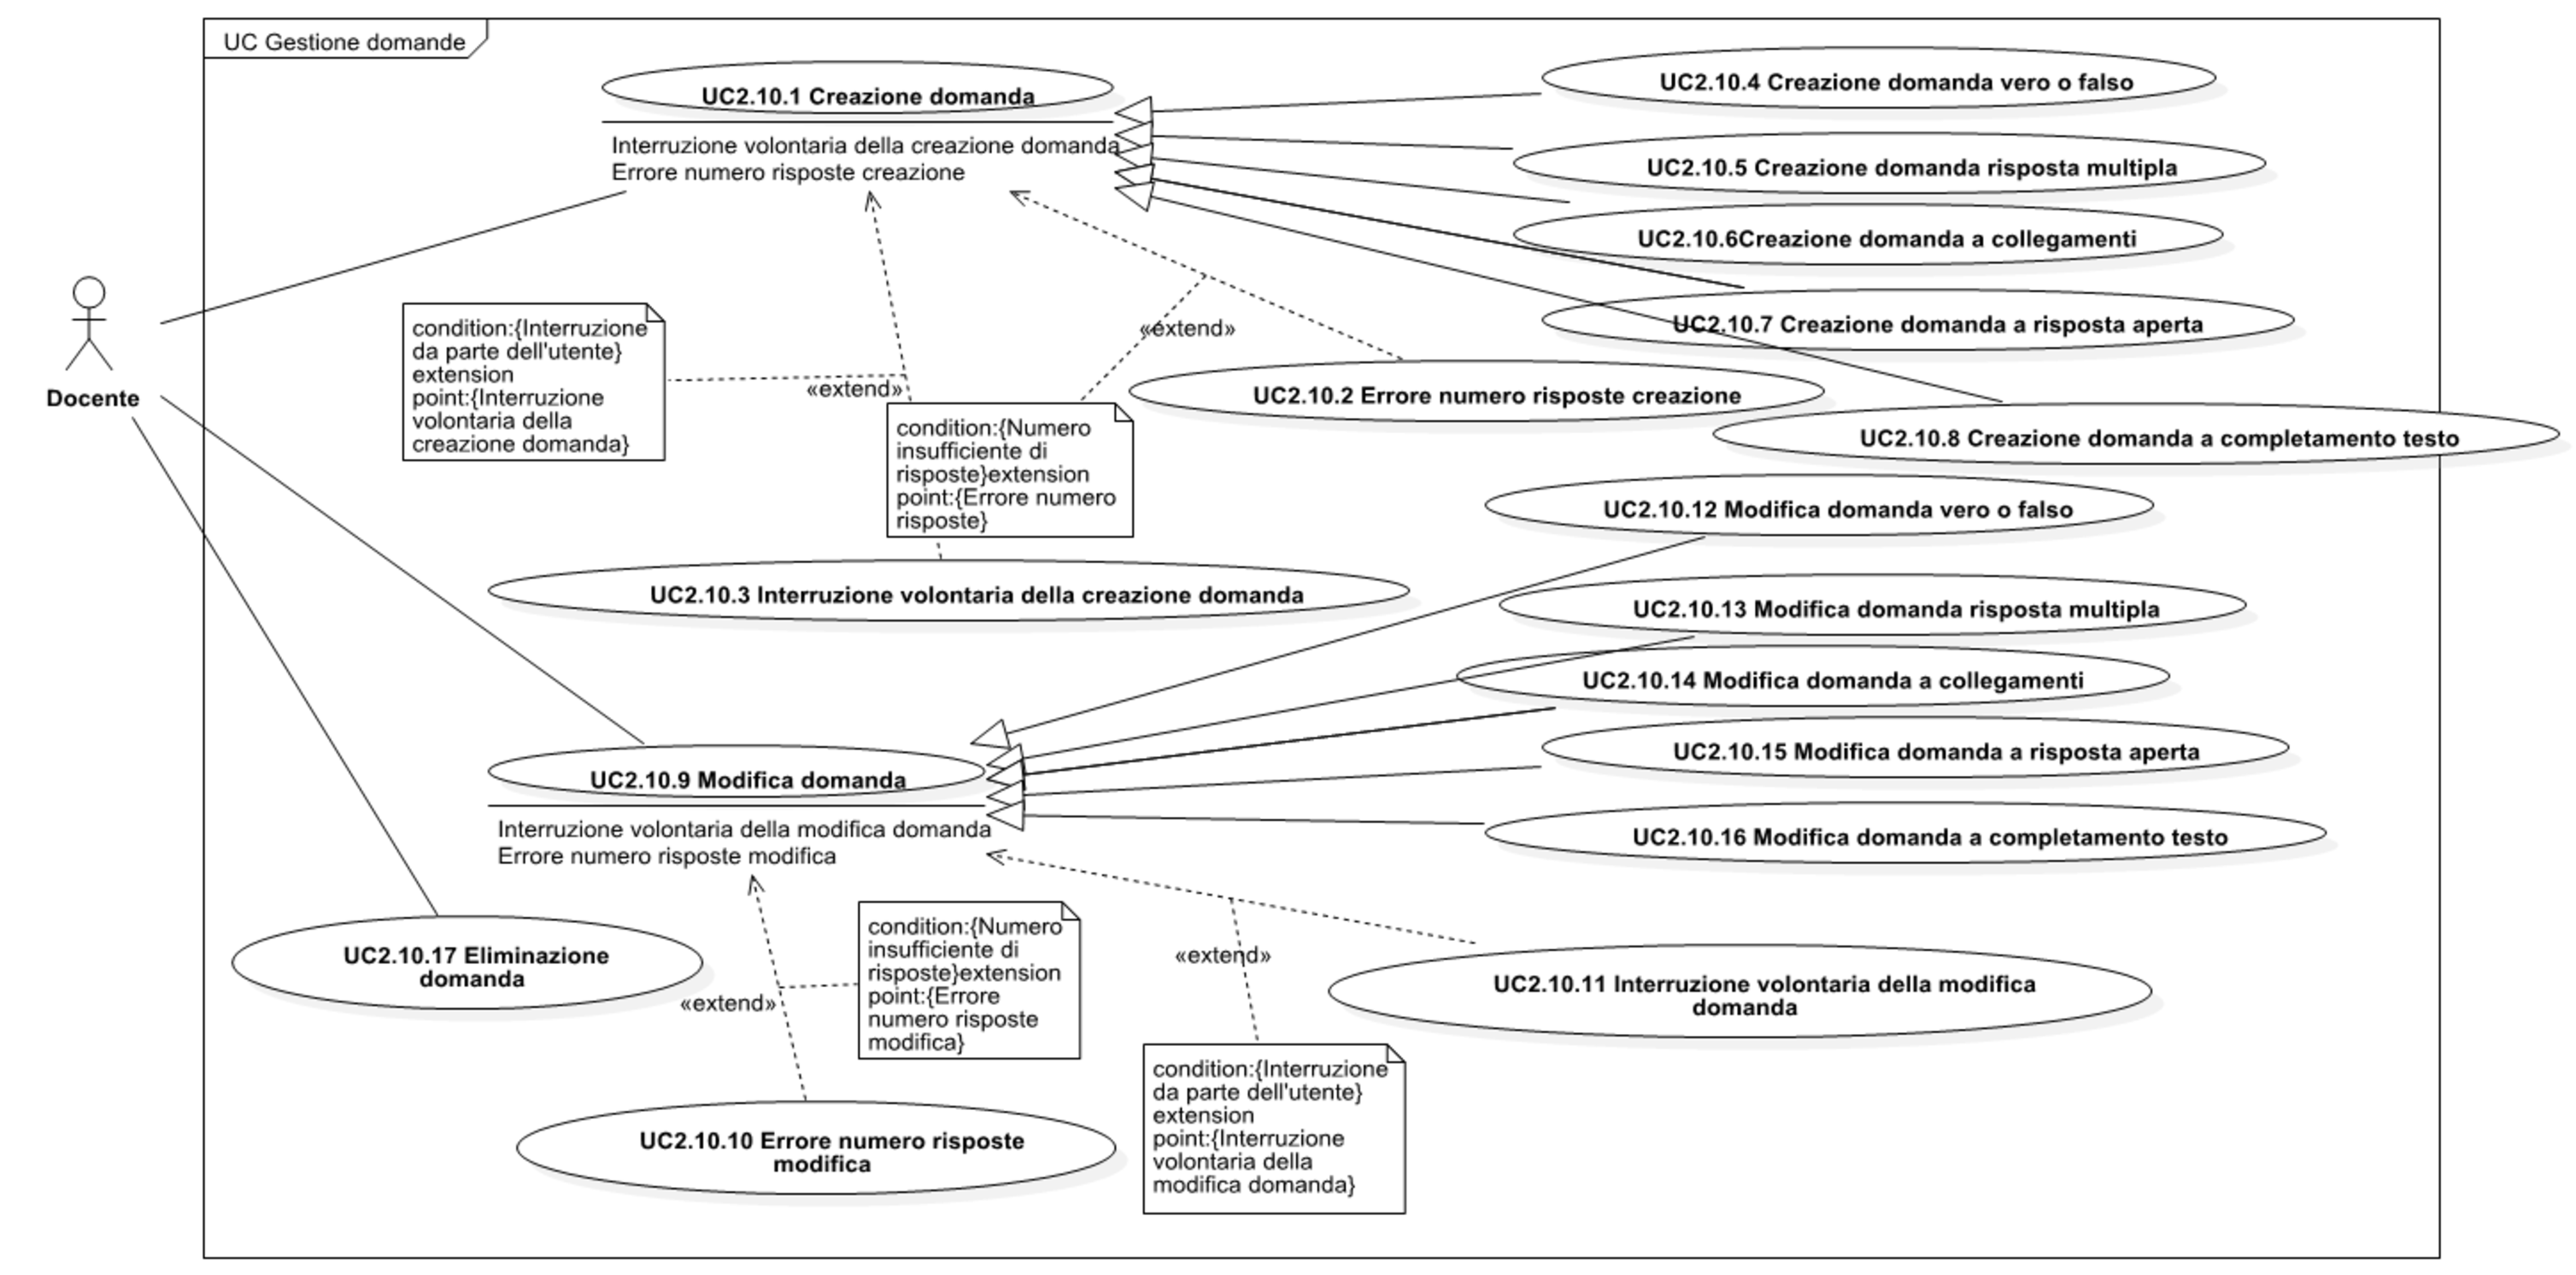
\includegraphics[width=\textwidth]{Img/UC Gestione domande.pdf}}
\caption{UC2.4 Gestione domande}
\end{figure}
\begin{itemize}
\item \textbf{Attori}: Docente.
\item \textbf{Scenario principale}:
\begin{enumerate}
\item Creazione domanda (UC2.4.1);
\item Modifica domanda vero o falso (UC2.4.2);
\item Modifica domanda a risposta multipla (UC2.4.3);
\item Modifica domanda a collegamenti (UC2.4.4);
\item Modifica domanda a risposta aperta (UC2.4.5);
\item Modifica domanda completamento testo (UC2.4.6);
\item Eliminazione domanda (UC2.4.7);
\item Modifica domanda (UC2.4.8).
\end{enumerate}
\item \textbf{Descrizione}: il docente deve poter effettuare varie operazioni sulle domande, in particolare deve poter creare nuove domande di vario tipo e modificare o eliminare domande esistenti.
\item \textbf{Precondizione}: il docente è autenticato e desidera gestire le domande.
\item \textbf{Postcondizione}: il docente ha effettuato le operazioni desiderate sulle domande.
\end{itemize}
\subsubsection{UC2.4.1 Creazione domanda}
\begin{figure}[H]
\centering
\noindent\makebox[\textwidth]{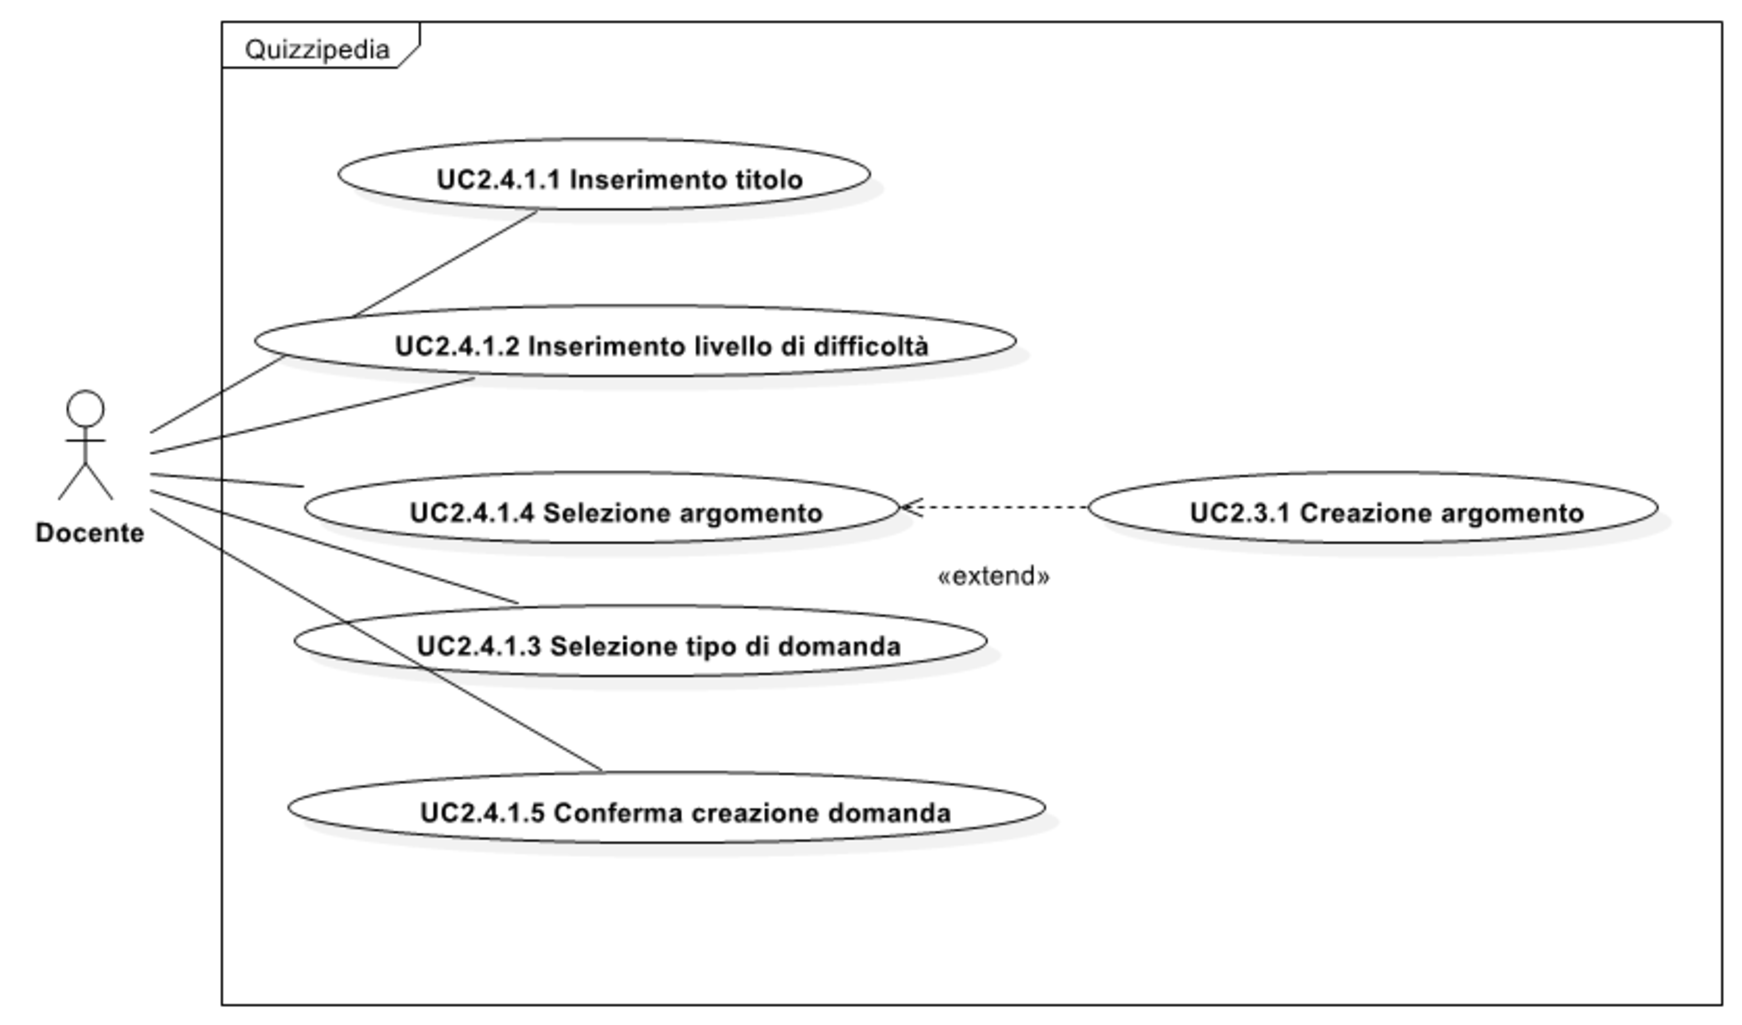
\includegraphics[width=\textwidth]{Img/UC Creazione domanda.pdf}}
\caption{UC2.4.1 Creazione domanda}
\end{figure}
\begin{itemize}
\item \textbf{Attori}: Docente.
\item \textbf{Scenario principale}:
\begin{enumerate}
\item Inserimento titolo domanda (UC2.4.1.1);
\item Inserimento livello di difficoltà  (UC2.4.1.2);
\item Selezione tipo della domanda (UC2.4.1.3);
\item Selezione argomento della domanda (UC2.4.1.4);
\item Conferma creazione domanda (UC2.4.1.5).
\end{enumerate}
\item \textbf{Scenario alternativo}: il docente ha interrotto la creazione della domanda.
\item \textbf{Inclusioni}:
\begin{itemize}
\item Modifica domanda (UC2.4.8).
\end{itemize}
\item \textbf{Descrizione}: il docente deve poter creare una nuova domanda.
\item \textbf{Precondizione}: il docente desidera creare una nuova domanda.
\item \textbf{Postcondizione}: il docente ha creato una nuova domanda.
\end{itemize}
\subsubsection{UC2.4.1.1 Inserimento titolo domanda}
\begin{itemize}
\item \textbf{Attori}: Docente.
\item \textbf{Descrizione}: il docente deve poter inserire il titolo della domanda.
\item \textbf{Precondizione}: il docente ha iniziato la creazione di una domanda e non ha ancora inserito il titolo.
\item \textbf{Postcondizione}: il docente ha inserito il titolo.
\end{itemize}
\subsubsection{UC2.4.1.2 Inserimento livello di difficoltà }
\begin{itemize}
\item \textbf{Attori}: Docente.
\item \textbf{Descrizione}: il docente deve poter inserire il livello di difficoltà della domanda.
\item \textbf{Precondizione}: il docente ha iniziato la creazione di una domanda e non ha ancora inserito il livello di difficoltà.
\item \textbf{Postcondizione}: il docente ha inserito il livello di difficoltà.
\end{itemize}
\subsubsection{UC2.4.1.3 Selezione tipo della domanda}
\begin{itemize}
\item \textbf{Attori}: Docente.
\item \textbf{Descrizione}: il docente deve poter selezionare il tipo della domanda che sta creando: vero/falso, risposta multipla, collegamenti, risposta aperta, testo a completamento.
\item \textbf{Precondizione}: il docente ha iniziato la creazione di una domanda e non ha ancora selezionato il tipo della domanda.
\item \textbf{Postcondizione}: il docente ha selezionato il tipo della domanda.
\end{itemize}
\subsubsection{UC2.4.1.4 Selezione argomento della domanda}
\begin{itemize}
\item \textbf{Attori}: Docente.
\item \textbf{Estensioni}:
\begin{itemize}
\item Creazione argomento (UC2.3.1).
\end{itemize}
\item \textbf{Descrizione}: il docente deve poter selezionare l'argomento della domanda.
\item \textbf{Precondizione}: il docente ha iniziato la creazione di una domanda e non ha ancora selezionato l'argomento.
\item \textbf{Postcondizione}: il docente ha selezionato l'argomento.
\end{itemize}
\subsubsection{UC2.4.1.5 Conferma creazione domanda}
\begin{itemize}
\item \textbf{Attori}: Docente.
\item \textbf{Descrizione}: il docente deve poter confermare la creazione della domanda.
\item \textbf{Precondizione}: il docente sta creando una domanda, ha inserito le informazioni necessarie e vuole confermare la creazione della domanda.
\item \textbf{Postcondizione}: il docente ha confermato la creazione della domanda.
\end{itemize}
\subsubsection{UC2.4.2 Modifica domanda vero o falso}
\begin{figure}[H]
\centering
\noindent\makebox[\textwidth]{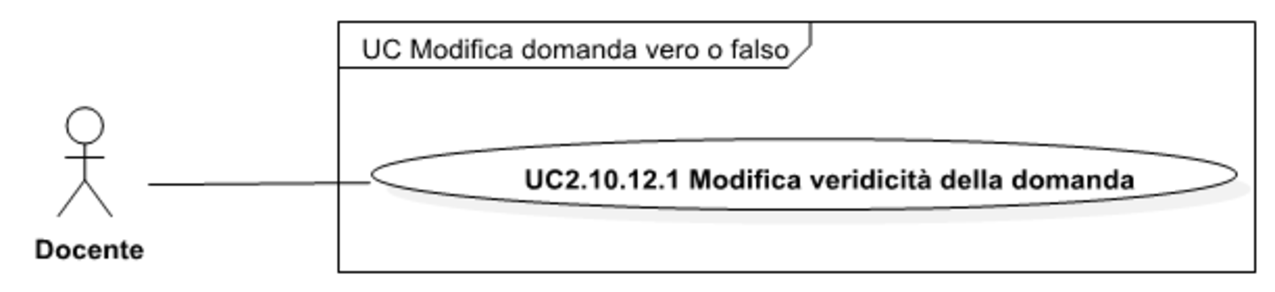
\includegraphics[width=\textwidth]{Img/UC Modifica domanda vero o falso.pdf}}
\caption{UC2.4.2 Modifica domanda vero o falso}
\end{figure}
\begin{itemize}
\item \textbf{Attori}: Docente.
\item \textbf{Scenario principale}:
\begin{enumerate}
\item Modifica veridicità della domanda (UC2.4.2.1).
\end{enumerate}
\item \textbf{Descrizione}: il docente può modificare una domanda di tipo vero/falso, cambiando la dichiarazione della veridicità della domanda. una domanda vero/falso è trattata come una singola domanda e non supporta l'inserimento di ulteriori risposte al suo interno, ma permette l'inserimento di caselle di testo e allegati nella descrizione.
\item \textbf{Precondizione}: il docente ha deciso di modificare una domanda di tipo vero/falso.
\item \textbf{Postcondizione}: il docente ha modificato la domanda di tipo vero/falso.
\item \textbf{Specializzazione di}:
\begin{enumerate}
\item Modifica domanda (UC2.4.8).
\end{enumerate}
\end{itemize}
\subsubsection{UC2.4.2.1 Modifica veridicità della domanda}
\begin{itemize}
\item \textbf{Attori}: Docente.
\item \textbf{Descrizione}: il docente deve poter modificare la veridicità della domanda, indicando se la risposta corretta è 'vero' oppure 'falso'.
\item \textbf{Precondizione}: il docente vuole modificare la veridicità della domanda.
\item \textbf{Postcondizione}: il docente ha modificato la veridicità della domanda.
\end{itemize}
\subsubsection{UC2.4.3 Modifica domanda a risposta multipla}
\begin{figure}[H]
\centering
\noindent\makebox[\textwidth]{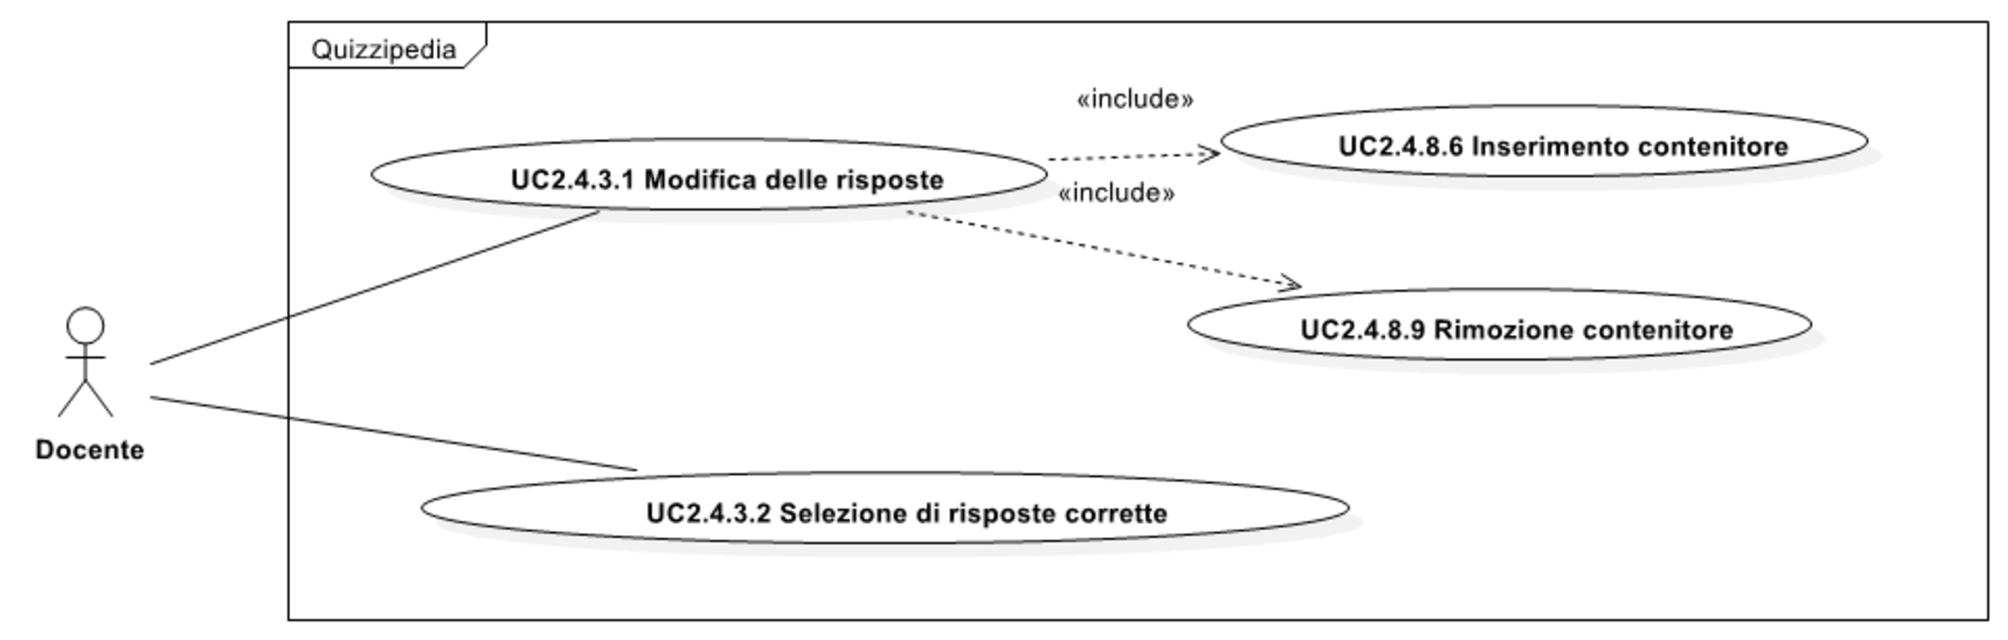
\includegraphics[width=\textwidth]{Img/UC Modifica domanda a risposta multipla.pdf}}
\caption{UC2.4.3 Modifica domanda a risposta multipla}
\end{figure}
\begin{itemize}
\item \textbf{Attori}: Docente.
\item \textbf{Scenario principale}:
\begin{enumerate}
\item Modifica delle risposte (UC2.4.3.1);
\item Selezione risposte corrette (UC2.4.3.2).
\end{enumerate}
\item \textbf{Descrizione}: il docente può modificare una domanda a risposta multipla.
\item \textbf{Precondizione}: il docente ha deciso di modificare una domanda a risposta multipla.
\item \textbf{Postcondizione}: il docente ha modificato la domanda a risposta multipla.
\item \textbf{Specializzazione di}:
\begin{enumerate}
\item Modifica domanda (UC2.4.8).
\end{enumerate}
\end{itemize}
\subsubsection{UC2.4.3.1 Modifica delle risposte}
\begin{itemize}
\item \textbf{Attori}: Docente.
\item \textbf{Inclusioni}:
\begin{itemize}
\item Inserimento contenitore (UC2.4.8.6);
\item Rimozione contenitore (UC2.4.8.9).
\end{itemize}
\item \textbf{Descrizione}: il docente può aggiungere o rimuovere le risposte inserite come risposte possibili, sia risposte corrette sia risposte errate. una risposta è rappresentata da un contenitore. L'interfaccia permetterà al docente di posizionare e ordinare le risposte entro i limiti imposti dal layout.
\item \textbf{Precondizione}: il docente ha deciso di modificare una domanda a risposta multipla.
\item \textbf{Postcondizione}: il docente ha modificato le risposte.
\end{itemize}
\subsubsection{UC2.4.3.2 Selezione risposte corrette}
\begin{itemize}
\item \textbf{Attori}: Docente.
\item \textbf{Descrizione}: l'interfaccia permetterà al docente di selezionare e deselezionare le risposte corrette fra quelle inserite. Selezionare una risposta la renderà corretta e deselezionarla la renderà errata. Il tipo di domanda 'risposta multipla' supporta la selezione di un numero corrette compreso fra 1 e il numero di risposte inserite.
\item \textbf{Precondizione}: il docente vuole modificare le risposte corrette di una domanda a risposta multipla.
\item \textbf{Postcondizione}: il docente ha modificato le risposte corrette.
\end{itemize}
\subsubsection{UC2.4.4 Modifica domanda a collegamenti}
\begin{figure}[H]
\centering
\noindent\makebox[\textwidth]{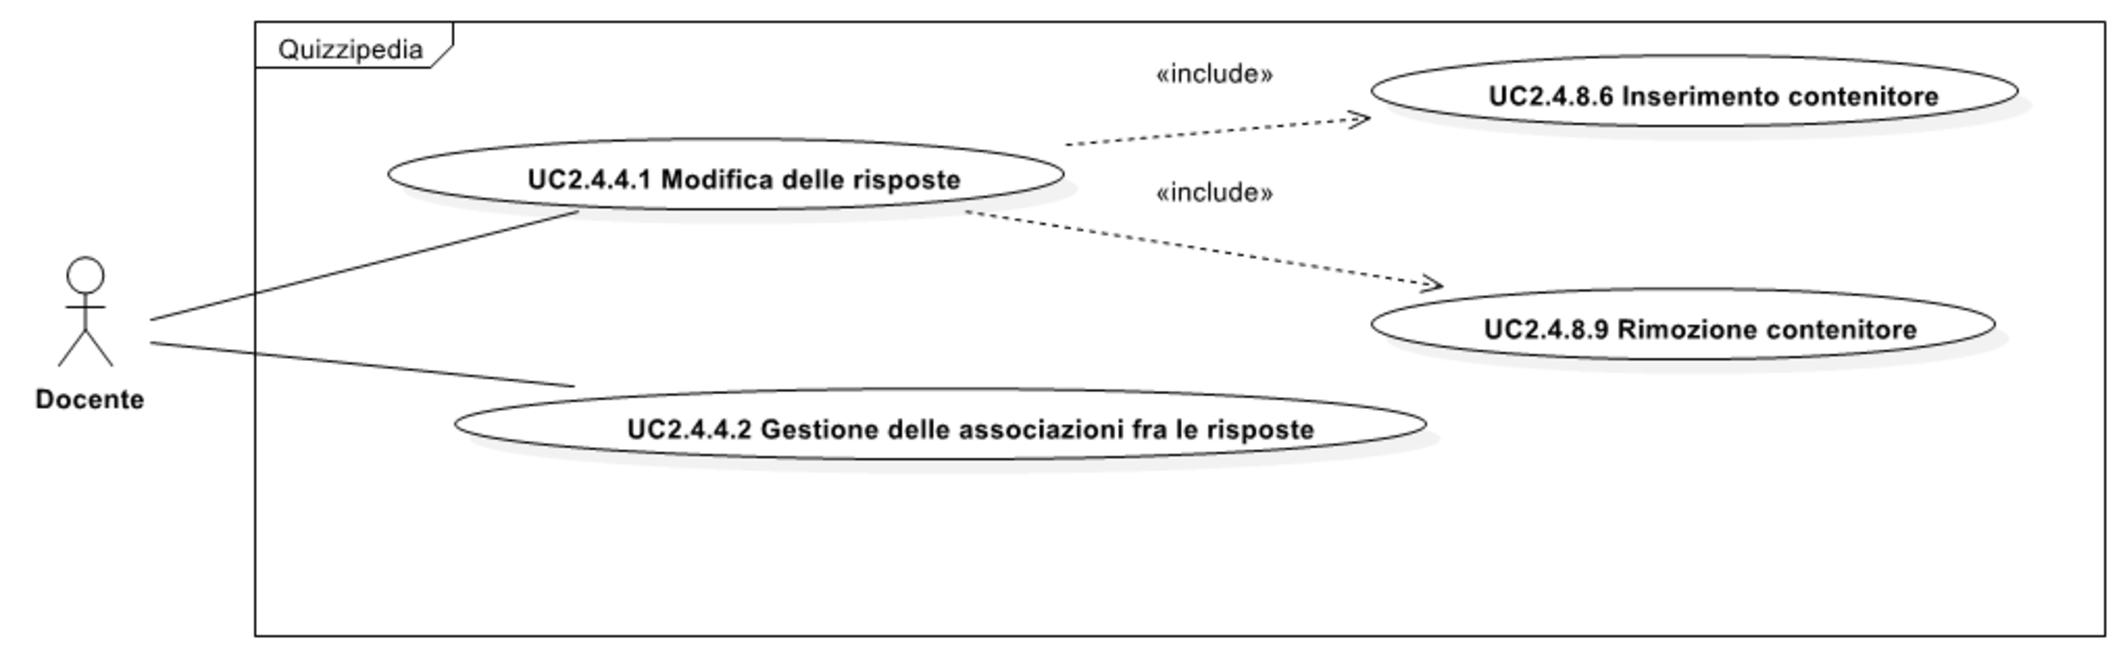
\includegraphics[width=\textwidth]{Img/UC Modifica domanda a collegamenti.pdf}}
\caption{UC2.4.4 Modifica domanda a collegamenti}
\end{figure}
\begin{itemize}
\item \textbf{Attori}: Docente.
\item \textbf{Scenario principale}:
\begin{enumerate}
\item Modifica delle risposte (UC2.4.4.1);
\item Gestione associazioni fra le risposte  (UC2.4.4.2).
\end{enumerate}
\item \textbf{Descrizione}: il docente può modificare una domanda a collegamenti. Una domanda a collegamenti è caratterizzata dalla possibilità di associare due contenitori, si possono così creare domande che richiedono l'ordinamento delle risposte e l'a creazione di associazioni fra diversi tipi di risposte (caselle di testo, immagini, file audio, file video) in qualsiasi combinazione. Le risposte possono essere ordinate e posizionate a piacere nei limiti consentiti dal layout della domanda.
\item \textbf{Precondizione}: il docente ha deciso di modificare una domanda a collegamenti.
\item \textbf{Postcondizione}: il docente ha modificato la domanda a collegamenti.
\item \textbf{Specializzazione di}:
\begin{enumerate}
\item Modifica domanda (UC2.4.8).
\end{enumerate}
\end{itemize}
\subsubsection{UC2.4.4.1 Modifica delle risposte}
\begin{itemize}
\item \textbf{Attori}: Docente.
\item \textbf{Inclusioni}:
\begin{itemize}
\item Inserimento contenitore (UC2.4.8.6);
\item Rimozione contenitore (UC2.4.8.9).
\end{itemize}
\item \textbf{Descrizione}: il docente può aggiungere o rimuovere le risposte inserite come risposte possibili, sia risposte corrette sia risposte errate. una risposta è rappresentata da un contenitore. L'interfaccia permetterà al docente di posizionare e ordinare le risposte entro i limiti imposti dal layout.
\item \textbf{Precondizione}: il docente sta modificando una domanda a collegamenti.
\item \textbf{Postcondizione}: il docente ha modificato le risposte .
\end{itemize}
\subsubsection{UC2.4.4.2 Gestione associazioni fra le risposte }
\begin{itemize}
\item \textbf{Attori}: Docente.
\item \textbf{Descrizione}: l'interfaccia permette al docente di creare o rimuovere un'associazione fra due risposte o più. Associare due risposte rende il loro collegamento corretto, rimuovere l'associazione rende il collegamento errato.
\item \textbf{Precondizione}: il docente ha deciso di modificare una domanda a collegamenti.
\item \textbf{Postcondizione}: il docente ha effettuato la gestione delle associazioni.
\end{itemize}
\subsubsection{UC2.4.5 Modifica domanda a risposta aperta}
\begin{figure}[H]
\centering
\noindent\makebox[\textwidth]{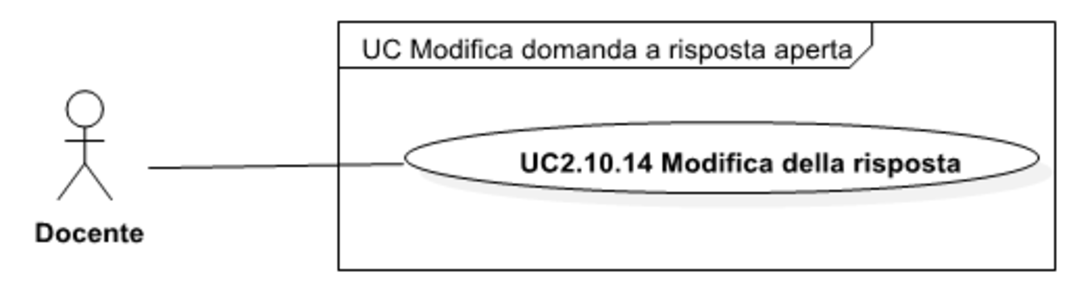
\includegraphics[width=\textwidth]{Img/UC Modifica domanda a risposta aperta.pdf}}
\caption{UC2.4.5 Modifica domanda a risposta aperta}
\end{figure}
\begin{itemize}
\item \textbf{Attori}: Docente.
\item \textbf{Scenario principale}:
\begin{enumerate}
\item Gestione risposta corretta (UC2.4.5.1).
\end{enumerate}
\item \textbf{Descrizione}: il docente può modificare una domanda a risposta aperta. non è possibile creare risposte, verrà creata automaticamente una casella di testo dove lo studente dovrà rispondere alla domanda. L'utilizzo di domande a risposta aperta è consigliato per domande che hanno risposte corte e prevedibili, come singole parole, nomi propri, nomi geografici, date e numeri.
\item \textbf{Precondizione}: il docente ha deciso di modificare una domanda a risposta aperta.
\item \textbf{Postcondizione}: il docente ha modificato la domanda a risposta aperta.
\item \textbf{Specializzazione di}:
\begin{enumerate}
\item Modifica domanda (UC2.4.8).
\end{enumerate}
\end{itemize}
\subsubsection{UC2.4.5.1 Gestione risposta corretta}
\begin{itemize}
\item \textbf{Attori}: Docente.
\item \textbf{Descrizione}: l'interfaccia permette al docente di inserire o modificare la risposta corretta in una casella di testo, la risposta dello studente verrà confrontata con questa.
\item \textbf{Precondizione}: il docente ha deciso di gestire la risposta corretta di una domanda a risposta aperta.
\item \textbf{Postcondizione}: il docente ha gestito la risposta corretta di una domanda a risposta aperta.
\end{itemize}
\subsubsection{UC2.4.6 Modifica domanda completamento testo}
\begin{figure}[H]
\centering
\noindent\makebox[\textwidth]{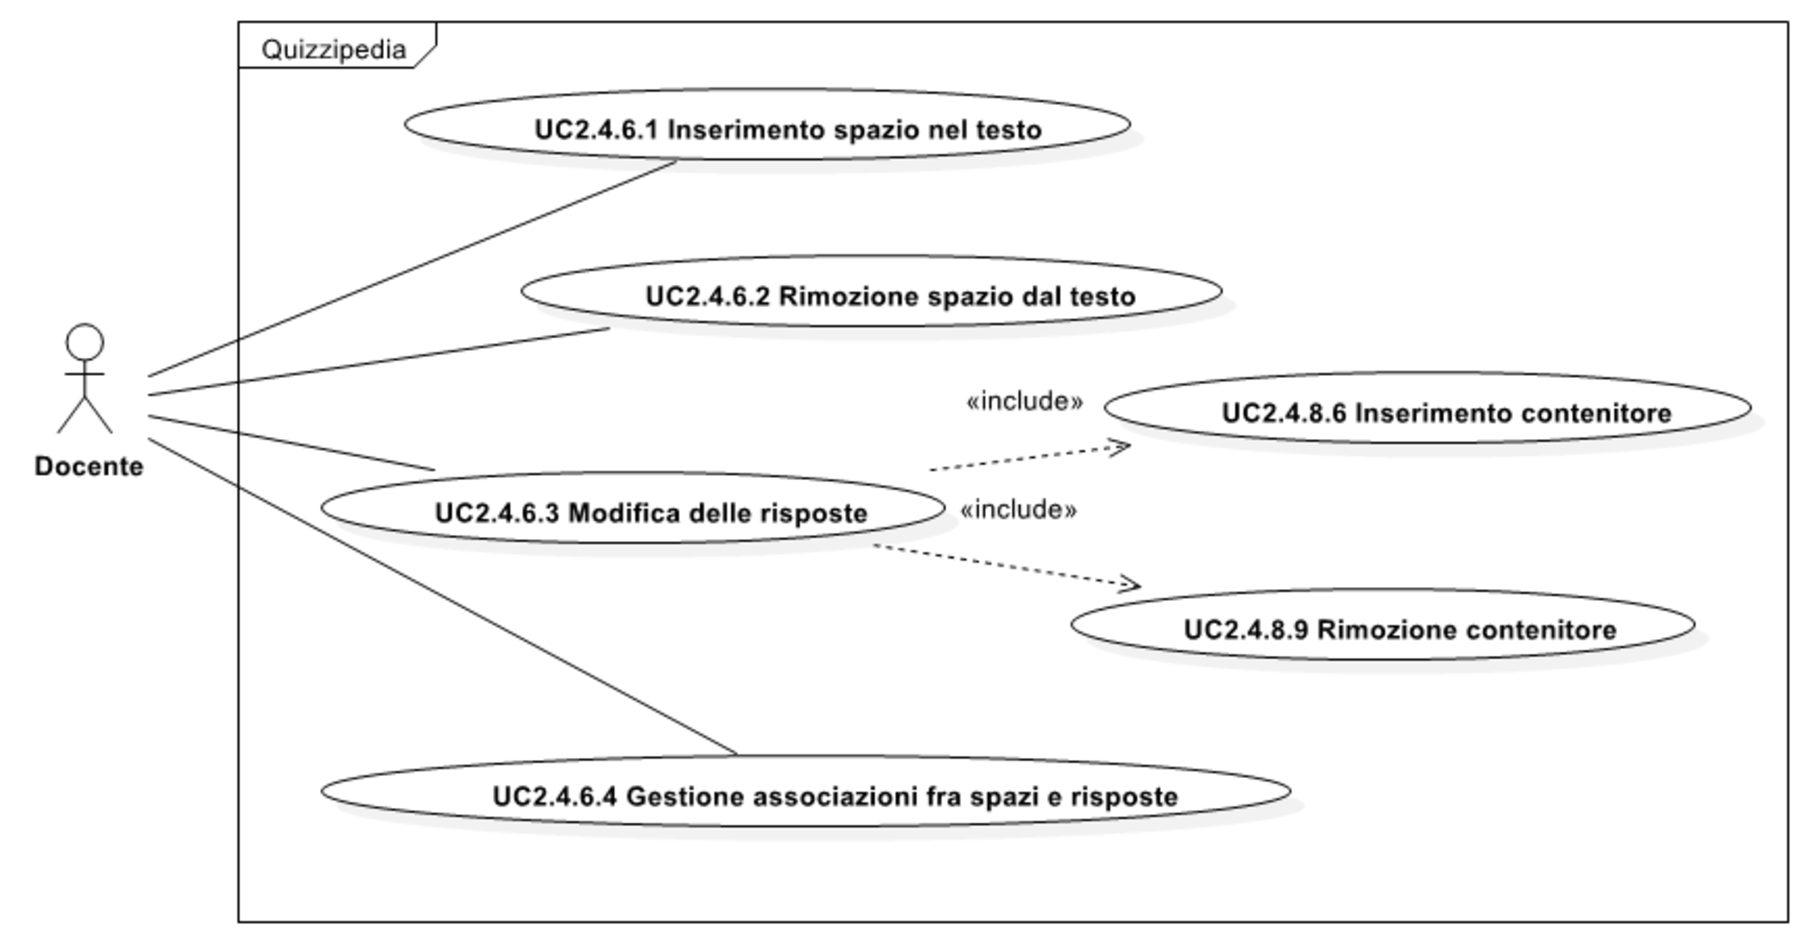
\includegraphics[width=\textwidth]{Img/UC Modifica domanda completamento testo.pdf}}
\caption{UC2.4.6 Modifica domanda completamento testo}
\end{figure}
\begin{itemize}
\item \textbf{Attori}: Docente.
\item \textbf{Scenario principale}:
\begin{enumerate}
\item Inserimento spazio nel testo (UC2.4.6.1);
\item Rimozione spazio dal testo (UC2.4.6.2);
\item Modifica delle risposte  (UC2.4.6.3);
\item Gestione associazioni fra spazi e risposte (UC2.4.6.4).
\end{enumerate}
\item \textbf{Inclusioni}:
\begin{itemize}
\item Inserimento contenitore (UC2.4.8.6);
\item Rimozione contenitore (UC2.4.8.9).
\end{itemize}
\item \textbf{Descrizione}: il docente può modificare una domanda di tipo 'completamento testo'. La struttura del testo dipende dai contenitori scelti per costruirlo, e può spaziare da una semplice casella di testo intervallata da spazi a una combinazione di testo e allegati.
\item \textbf{Precondizione}: il docente ha deciso di modificare una domanda di tipo 'completamento testo'.
\item \textbf{Postcondizione}: il docente ha modificato la domanda di tipo 'completamento testo'.
\item \textbf{Specializzazione di}:
\begin{enumerate}
\item Modifica domanda (UC2.4.8).
\end{enumerate}
\end{itemize}
\subsubsection{UC2.4.6.1 Inserimento spazio nel testo}
\begin{itemize}
\item \textbf{Attori}: Docente.
\item \textbf{Descrizione}: l'interfaccia permette al docente di inserire un nuovo spazio nel testo, nella posizione da lui scelta.
\item \textbf{Precondizione}: il docente ha deciso di inserire un nuovo spazio nel testo.
\item \textbf{Postcondizione}: il docente ha inserito lo spazio nel testo.
\end{itemize}
\subsubsection{UC2.4.6.2 Rimozione spazio dal testo}
\begin{itemize}
\item \textbf{Attori}: Docente.
\item \textbf{Descrizione}: l'interfaccia permette al docente di rimuovere uno spazio scelto dal testo.
\item \textbf{Precondizione}: il docente ha deciso di rimuovere uno spazio dal testo.
\item \textbf{Postcondizione}: il docente ha rimosso lo spazio dal testo.
\end{itemize}
\subsubsection{UC2.4.6.3 Modifica delle risposte }
\begin{itemize}
\item \textbf{Attori}: Docente.
\item \textbf{Inclusioni}:
\begin{itemize}
\item Inserimento contenitore (UC2.4.8.6);
\item Rimozione contenitore (UC2.4.8.9).
\end{itemize}
\item \textbf{Descrizione}: il docente può aggiungere o rimuovere risposte. Le risposte possono essere di tipo testuale o allegato (immagine, file audio, file video).
\item \textbf{Precondizione}: il docente ha deciso di modificare una domanda completamento testo.
\item \textbf{Postcondizione}: il docente ha modificato le risposte.
\end{itemize}
\subsubsection{UC2.4.6.4 Gestione associazioni fra spazi e risposte}
\begin{itemize}
\item \textbf{Attori}: Docente.
\item \textbf{Descrizione}: il docente può creare o rimuovere un'associazione fra una risposta e uno spazio. Se una risposta e uno spazio sono associati, posizionare la risposta nello spazio è considerato corretto o se una risposta e uno spazio non sono associati, posizionare la risposta nello spazio è considerato errato.
\item \textbf{Precondizione}: il docente ha deciso di modificare una domanda di tipo completamento testo.
\item \textbf{Postcondizione}: il docente ha effettuato la gestione delle associazioni in una domanda di tipo completamento testo.
\end{itemize}
\subsubsection{UC2.4.7 Eliminazione domanda}
\begin{figure}[H]
\centering
\noindent\makebox[\textwidth]{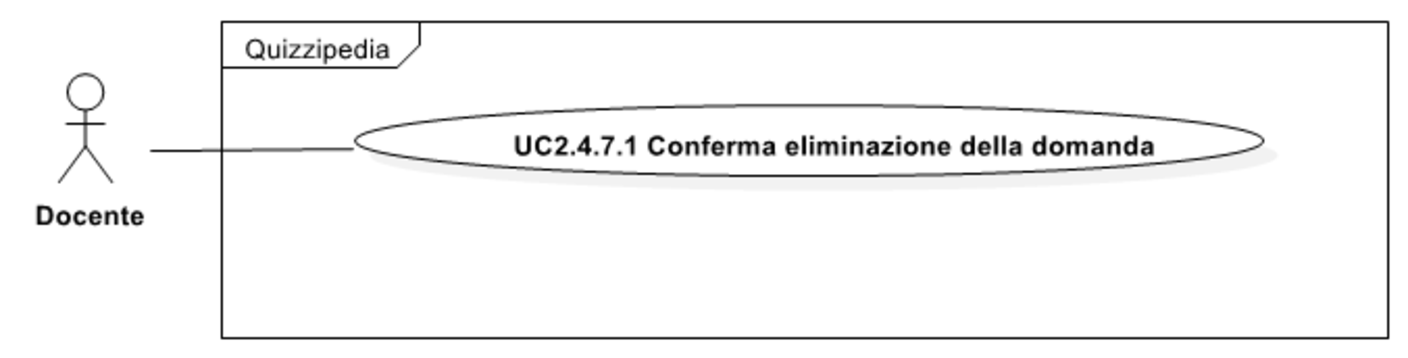
\includegraphics[width=\textwidth]{Img/UC Eliminazione domanda.pdf}}
\caption{UC2.4.7 Eliminazione domanda}
\end{figure}
\begin{itemize}
\item \textbf{Attori}: Docente.
\item \textbf{Scenario principale}:
\begin{enumerate}
\item Conferma eliminazione domanda (UC2.4.7.1).
\end{enumerate}
\item \textbf{Descrizione}: il docente può eliminare una domanda.
\item \textbf{Precondizione}: il docente vuole eliminare  una domanda.
\item \textbf{Postcondizione}: il docente ha eliminato la domanda.
\end{itemize}
\subsubsection{UC2.4.7.1 Conferma eliminazione domanda}
\begin{itemize}
\item \textbf{Attori}: Docente.
\item \textbf{Descrizione}: il docente confermare l'eliminazione della domanda affinchè l'operazione venga portata a termine. I docenti che hanno precedente inserito la domanda nei loro quiz riceveranno una notifica automatica e saranno invitati a controllare i quiz interessati.
\item \textbf{Precondizione}: il docente vuole eliminare una domanda.
\item \textbf{Postcondizione}: il docente ha confermato l'eliminazione della domanda.
\end{itemize}
\subsubsection{UC2.4.8 Modifica domanda}
\begin{figure}[H]
\centering
\noindent\makebox[\textwidth]{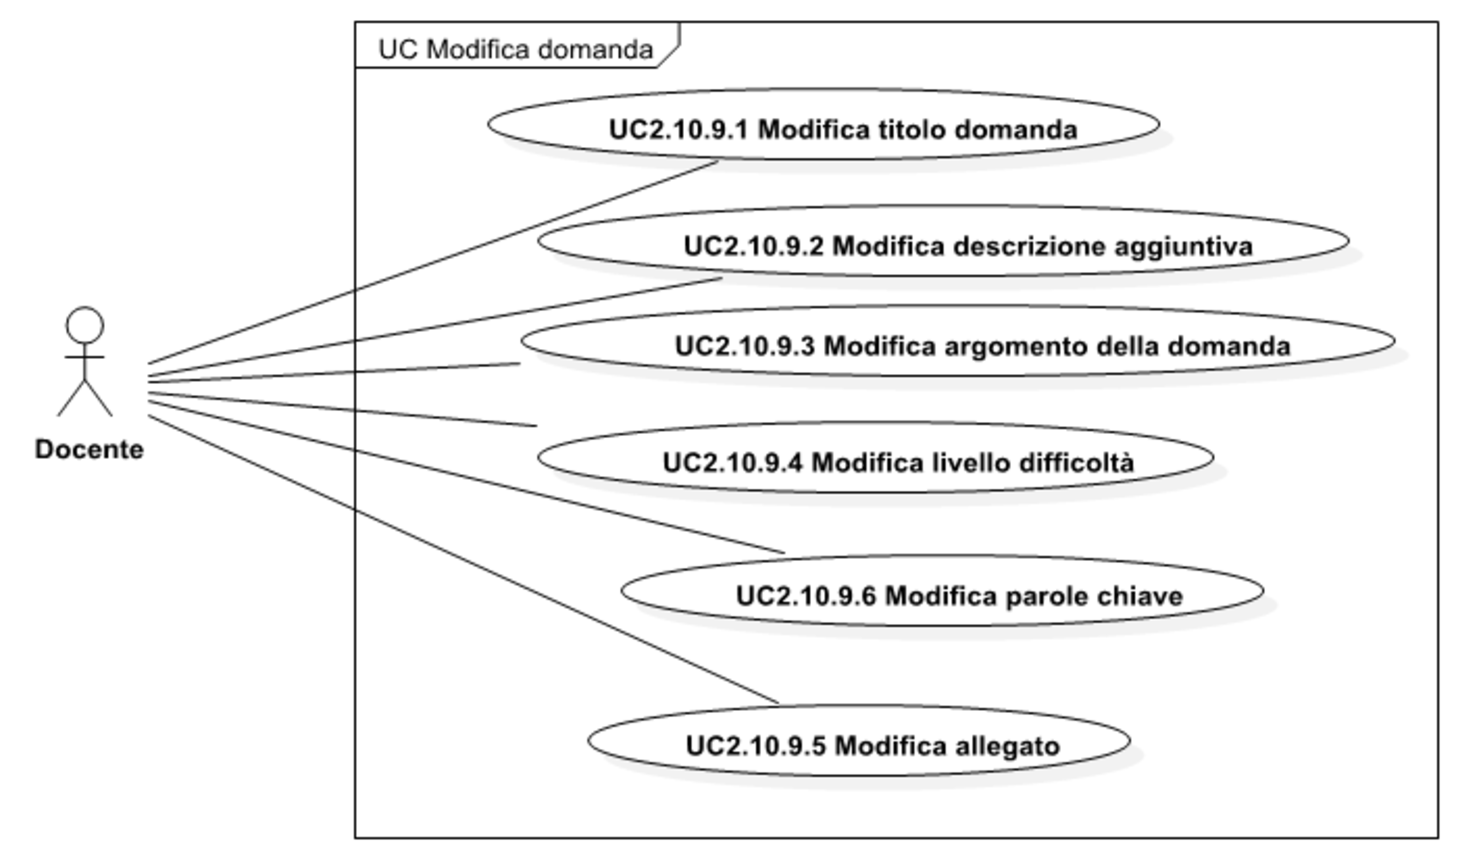
\includegraphics[width=\textwidth]{Img/UC Modifica domanda.pdf}}
\caption{UC2.4.8 Modifica domanda}
\end{figure}
\begin{itemize}
\item \textbf{Attori}: Docente.
\item \textbf{Scenario principale}:
\begin{enumerate}
\item Modifica titolo domanda (UC2.4.8.1);
\item Modifica livello di difficoltà  (UC2.4.8.2);
\item Modifica tipo della domanda (UC2.4.8.3);
\item Modifica argomento della domanda (UC2.4.8.4);
\item Gestione descrizione aggiuntiva della domanda (UC2.4.8.5);
\item Inserimento contenitore (UC2.4.8.6);
\item Inserimento casella di testo (UC2.4.8.7);
\item Inserimento allegato (UC2.4.8.8);
\item Rimozione contenitore (UC2.4.8.9);
\item Errore durante la modifica della domanda (UC2.4.8.10);
\item Conferma modifica domanda (UC2.4.8.11).
\end{enumerate}
\item \textbf{Scenario alternativo}: il docente interrompe la modifica della domanda.
\item \textbf{Estensioni}:
\begin{itemize}
\item Rimozione contenitore (UC2.4.8.9).
\end{itemize}
\item \textbf{Generalizzazioni}:
\begin{itemize}
\item Modifica domanda vero o falso (UC2.4.2);
\item Modifica domanda a risposta multipla (UC2.4.3);
\item Modifica domanda a collegamenti (UC2.4.4);
\item Modifica domanda a risposta aperta (UC2.4.5);
\item Modifica domanda completamento testo (UC2.4.6).
\end{itemize}
\item \textbf{Descrizione}: il docente deve poter modificare una domanda.
\item \textbf{Precondizione}: il docente desidera modificare una domanda.
\item \textbf{Postcondizione}: il docente ha modificato la domanda.
\end{itemize}
\subsubsection{UC2.4.8.1 Modifica titolo domanda}
\begin{itemize}
\item \textbf{Attori}: Docente.
\item \textbf{Descrizione}: il docente deve poter modificare il titolo della domanda.
\item \textbf{Precondizione}: il docente ha iniziato la modifica di una domanda.
\item \textbf{Postcondizione}: il docente ha modificato il titolo.
\end{itemize}
\subsubsection{UC2.4.8.2 Modifica livello di difficoltà }
\begin{itemize}
\item \textbf{Attori}: Docente.
\item \textbf{Descrizione}: il docente deve poter modificare il livello di difficoltà della domanda.
\item \textbf{Precondizione}: il docente ha iniziato la modifica di una domanda.
\item \textbf{Postcondizione}: il docente ha modificato il livello di difficoltà.
\end{itemize}
\subsubsection{UC2.4.8.3 Modifica tipo della domanda}
\begin{itemize}
\item \textbf{Attori}: Docente.
\item \textbf{Descrizione}: il docente deve poter modificare il tipo della domanda selezionato: vero/falso, risposta multipla, collegamenti, risposta aperta, testo a completamento.
\item \textbf{Precondizione}: il docente ha iniziato la modifica di una domanda.
\item \textbf{Postcondizione}: il docente ha modificato il tipo della domanda.
\end{itemize}
\subsubsection{UC2.4.8.4 Modifica argomento della domanda}
\begin{itemize}
\item \textbf{Attori}: Docente.
\item \textbf{Estensioni}:
\begin{itemize}
\item Creazione argomento (UC2.3.1).
\end{itemize}
\item \textbf{Descrizione}: il docente deve poter modificare l'argomento della domanda.
\item \textbf{Precondizione}: il docente ha iniziato la modifica di una domanda.
\item \textbf{Postcondizione}: il docente ha modificato l'argomento.
\end{itemize}
\subsubsection{UC2.4.8.5 Gestione descrizione aggiuntiva della domanda}
\begin{itemize}
\item \textbf{Attori}: Docente.
\item \textbf{Inclusioni}:
\begin{itemize}
\item Inserimento contenitore (UC2.4.8.6);
\item Rimozione contenitore (UC2.4.8.9).
\end{itemize}
\item \textbf{Descrizione}: il docente deve poter inserire e successivamente modificare una descrizione aggiuntiva che può contenere un numero variabile di 'contenitori', che possono essere caselle di testo o allegati (immagini, file audio, file video).
\item \textbf{Precondizione}: il docente sta modificando una domanda.
\item \textbf{Postcondizione}: il docente ha modificato la descrizione aggiuntiva.
\end{itemize}
\subsubsection{UC2.4.8.6 Inserimento contenitore}
\begin{itemize}
\item \textbf{Attori}: Docente.
\item \textbf{Generalizzazioni}:
\begin{itemize}
\item Inserimento casella di testo (UC2.4.8.7);
\item Inserimento allegato (UC2.4.8.8).
\end{itemize}
\item \textbf{Descrizione}: il docente può inserire un 'contenitore' in varie sezioni della domanda. Un contenitore può essere una casella di testo o un allegato (immagine, file audio, file video).
\item \textbf{Precondizione}: il docente sta modificando una domanda e vuole inserire un contenitore in una sezione della domanda.
\item \textbf{Postcondizione}: il docente ha inserito il contenitore nella sezione desiderata.
\end{itemize}
\subsubsection{UC2.4.8.7 Inserimento casella di testo}
\begin{itemize}
\item \textbf{Attori}: Docente.
\item \textbf{Descrizione}: il docente può inserire una casella di testo in varie sezioni della domanda.
\item \textbf{Precondizione}: il docente sta modificando una domanda e vuole inserire una casella di testo.
\item \textbf{Postcondizione}: il docente ha inserito la casella di testo nella sezione desiderata.
\item \textbf{Specializzazione di}:
\begin{enumerate}
\item Inserimento contenitore (UC2.4.8.6).
\end{enumerate}
\end{itemize}
\subsubsection{UC2.4.8.8 Inserimento allegato}
\begin{figure}[H]
\centering
\noindent\makebox[\textwidth]{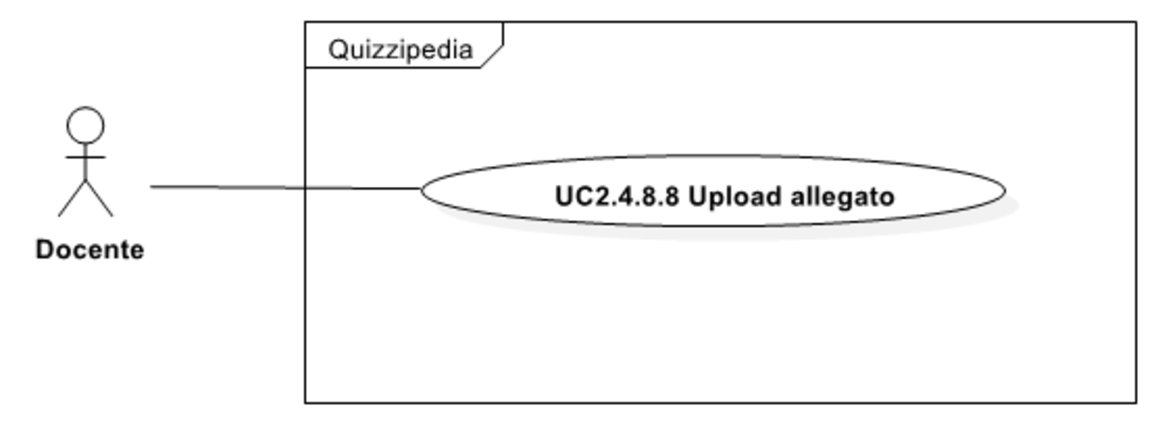
\includegraphics[width=\textwidth]{Img/UC Inserimento allegato.pdf}}
\caption{UC2.4.8.8 Inserimento allegato}
\end{figure}
\begin{itemize}
\item \textbf{Attori}: Docente.
\item \textbf{Scenario principale}:
\begin{enumerate}
\item Upload allegato (UC2.4.8.8.1).
\end{enumerate}
\item \textbf{Descrizione}: il docente può inserire un allegato (immagine, audio, video) in varie sezioni della domanda.
\item \textbf{Precondizione}: il docente sta modificando una domanda e vuole inserire un allegato.
\item \textbf{Postcondizione}: il docente ha inserito l'allegato nella sezione desiderata.
\item \textbf{Specializzazione di}:
\begin{enumerate}
\item Inserimento contenitore (UC2.4.8.6).
\end{enumerate}
\end{itemize}
\subsubsection{UC2.4.8.8.1 Upload allegato}
\begin{itemize}
\item \textbf{Attori}: Docente.
\item \textbf{Descrizione}: il docente può effettuare l'upload dell'allegato, secondo alcuni limiti.
\item \textbf{Precondizione}: il docente sta modificando una domanda e vuole effettuare l'upload dell'allegato.
\item \textbf{Postcondizione}: il docente ha inserito la casella di testo nella sezione desiderata.
\end{itemize}
\subsubsection{UC2.4.8.9 Rimozione contenitore}
\begin{itemize}
\item \textbf{Attori}: Docente.
\item \textbf{Descrizione}: il docente può rimuovere un contenitore precedentemente inserito.
\item \textbf{Precondizione}: il docente sta modificando una domanda e vuole rimuovere un contenitore.
\item \textbf{Postcondizione}: il docente ha rimosso il contenitore.
\end{itemize}
\subsubsection{UC2.4.8.10 Errore durante la modifica della domanda}
\begin{itemize}
\item \textbf{Attori}: Docente.
\item \textbf{Descrizione}: la seguente condizione si è verificata: eccessivo numero di contenitori inserito
.
\item \textbf{Precondizione}: il docente ha effettuato un tentativo di modifica di una domanda che non è andato a buon fine.
\item \textbf{Postcondizione}: il docente ha visualizzato l'errore.
\end{itemize}
\subsubsection{UC2.4.8.11 Conferma modifica domanda}
\begin{itemize}
\item \textbf{Attori}: Docente.
\item \textbf{Descrizione}: il docente deve poter confermare le modifiche apportate alla domanda, a prescindere dal tipo della domanda.
\item \textbf{Precondizione}: il docente sta modificando una domanda e vuole confermare la modifica della domanda.
\item \textbf{Postcondizione}: il docente ha confermato la modifica della domanda.
\end{itemize}
\subsubsection{UC2.5 Gestione account}
\begin{figure}[H]
\centering
\noindent\makebox[\textwidth]{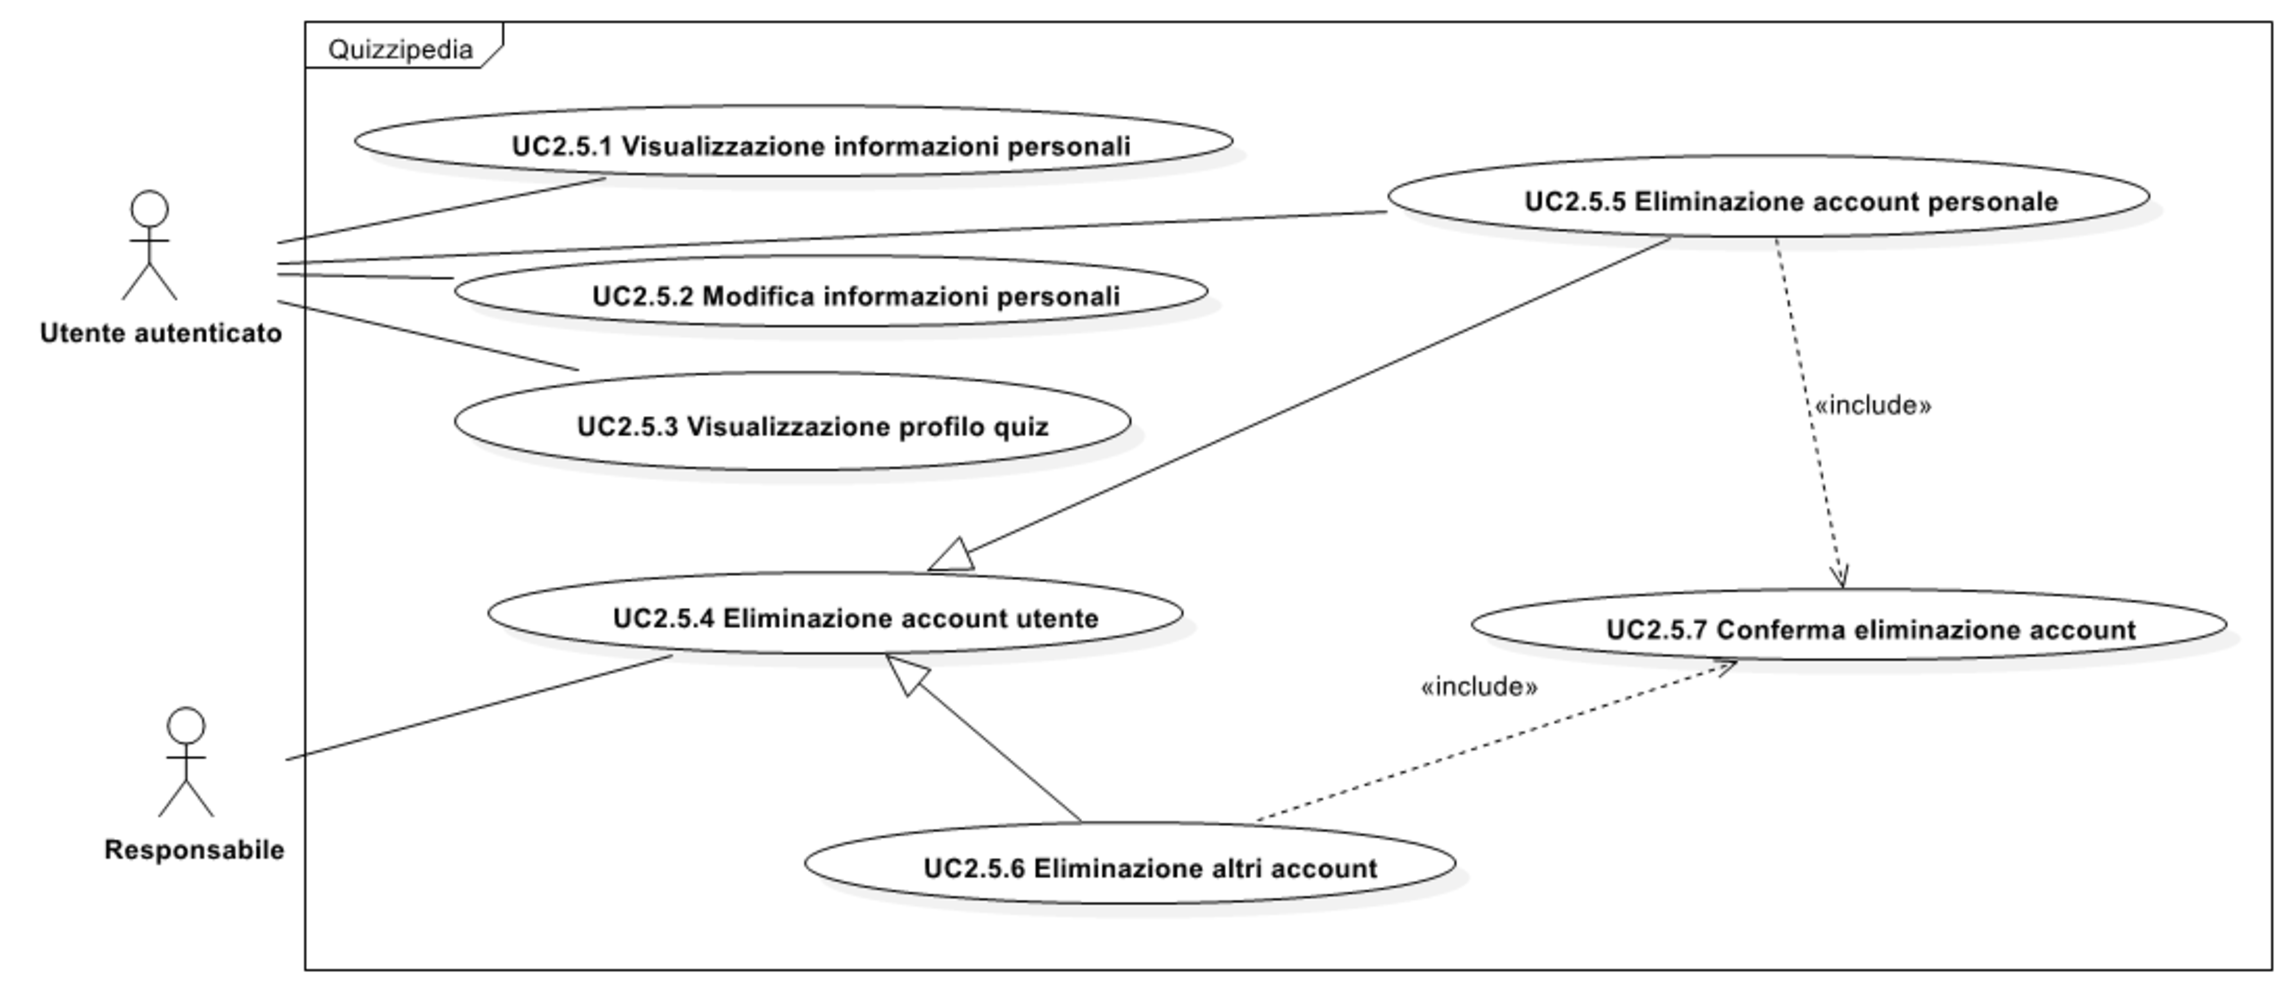
\includegraphics[width=\textwidth]{Img/UC Gestione account.pdf}}
\caption{UC2.5 Gestione account}
\end{figure}
\begin{itemize}
\item \textbf{Attori}: Responsabile, Utente Autenticato.
\item \textbf{Scenario principale}:
\begin{enumerate}
\item Visualizzazione informazioni personali (UC2.5.1);
\item Modifica informazioni personali (UC2.5.2);
\item Visualizzazione profilo quiz (UC2.5.3);
\item Eliminazione account utente (UC2.5.4);
\item Eliminazione account personale (UC2.5.5);
\item Eliminazione altri account (UC2.5.6);
\item Conferma eliminazione account (UC2.5.7).
\end{enumerate}
\item \textbf{Descrizione}: L'utente autenticato può visualizzare e modificare le sue informazioni personali; visualizzare il proprio profilo quiz e la possibilità di eliminare il proprio account. Il responsabile in aggiunta può eliminare gli account degli utenti.
\item \textbf{Precondizione}: il responsabile o un utente autorizzato vuole modificare/visualizzare le informazioni del proprio account.
\item \textbf{Postcondizione}: l'utente autenticato o il responsabile hanno effettuato le modifiche opportune al proprio account.
\end{itemize}
\subsubsection{UC2.5.1 Visualizzazione informazioni personali}
\begin{figure}[H]
\centering
\noindent\makebox[\textwidth]{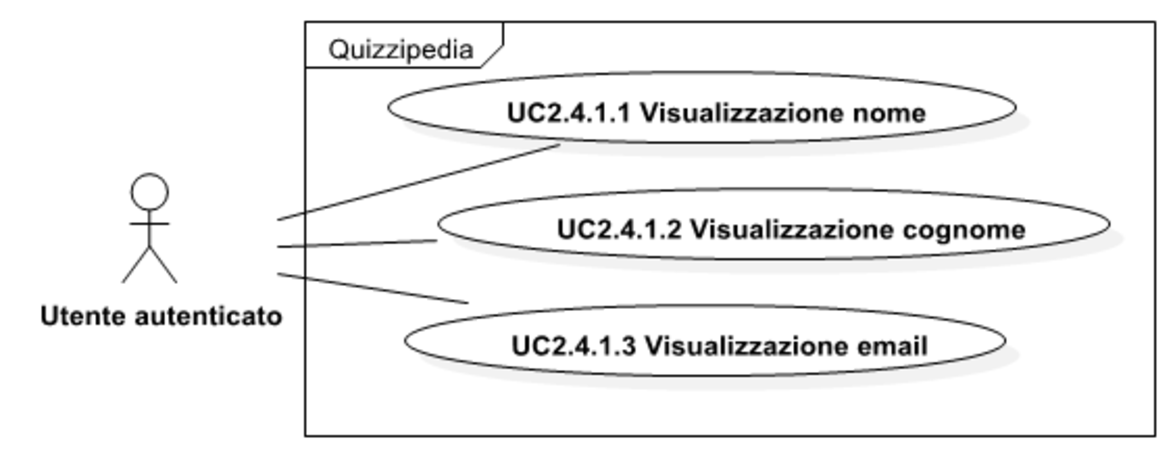
\includegraphics[width=\textwidth]{Img/UC Visualizzazione informazioni personali.pdf}}
\caption{UC2.5.1 Visualizzazione informazioni personali}
\end{figure}
\begin{itemize}
\item \textbf{Attori}: Utente Autenticato.
\item \textbf{Scenario principale}:
\begin{enumerate}
\item Visualizzazione nome (UC2.5.1.1);
\item Visualizzazione cognome (UC2.5.1.2);
\item Visualizzazione email (UC2.5.1.3).
\end{enumerate}
\item \textbf{Descrizione}: l'utente autenticato può visualizzare le sue informazioni personali.
\item \textbf{Precondizione}: l'utente autenticato ha l'accesso alla gestione dell'account.
\item \textbf{Postcondizione}: l'utente autenticato ha visualizzato le sue informazioni personali.
\end{itemize}
\subsubsection{UC2.5.1.1 Visualizzazione nome}
\begin{itemize}
\item \textbf{Attori}: Utente Autenticato.
\item \textbf{Descrizione}: l'utente autenticato visualizza il suo nome.
\item \textbf{Precondizione}: l'utente sta visualizzando le sue informazioni personali.
\item \textbf{Postcondizione}: l'utente visualizza il proprio nome.
\end{itemize}
\subsubsection{UC2.5.1.2 Visualizzazione cognome}
\begin{itemize}
\item \textbf{Attori}: Utente Autenticato.
\item \textbf{Descrizione}: l'utente autenticato visualizza il suo cognome.
\item \textbf{Precondizione}: l'utente sta visualizzando le sue informazioni personali.
\item \textbf{Postcondizione}: l'utente visualizza il proprio cognome.
\end{itemize}
\subsubsection{UC2.5.1.3 Visualizzazione email}
\begin{itemize}
\item \textbf{Attori}: Utente Autenticato.
\item \textbf{Descrizione}: l'utente autenticato visualizza la sua email.
\item \textbf{Precondizione}: l'utente sta visualizzando le sue informazioni personali.
\item \textbf{Postcondizione}: l'utente visualizza la propria email.
\end{itemize}
\subsubsection{UC2.5.2 Modifica informazioni personali}
\begin{figure}[H]
\centering
\noindent\makebox[\textwidth]{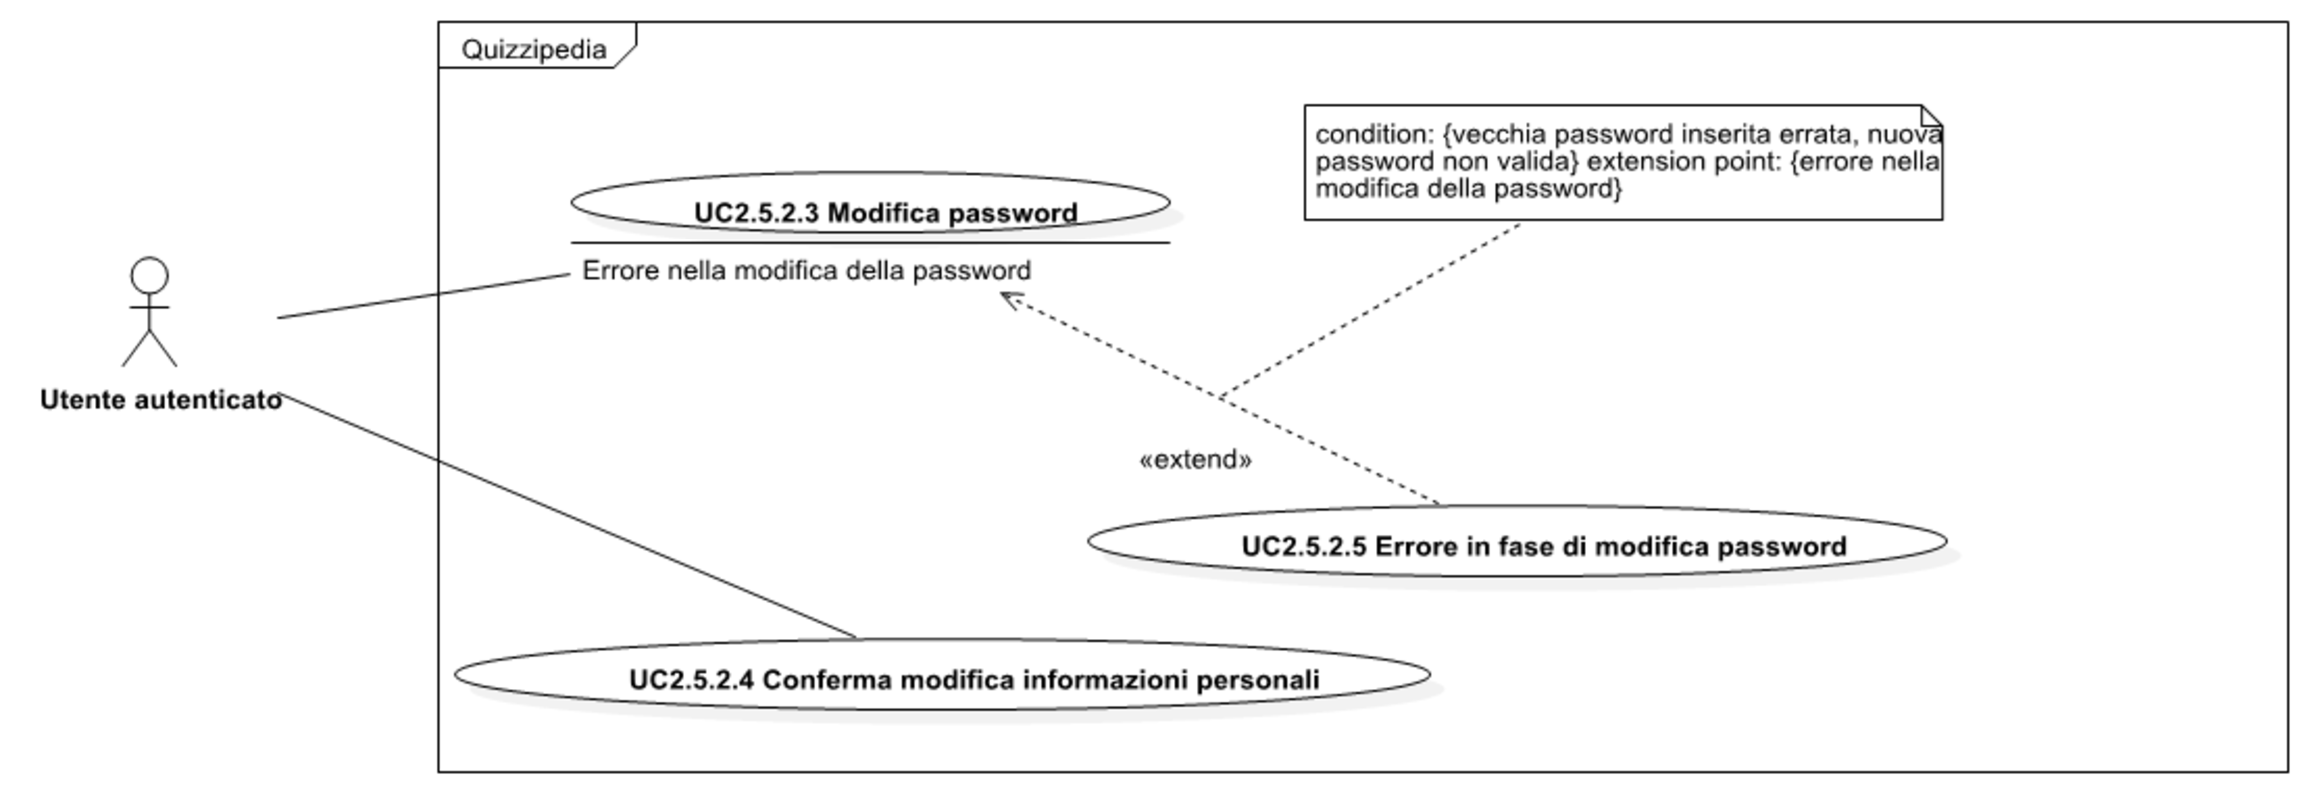
\includegraphics[width=\textwidth]{Img/UC Modifica informazioni personali.pdf}}
\caption{UC2.5.2 Modifica informazioni personali}
\end{figure}
\begin{itemize}
\item \textbf{Attori}: Utente Autenticato.
\item \textbf{Scenario principale}:
\begin{enumerate}
\item Modifica nome (UC2.5.2.1);
\item Modifica cognome (UC2.5.2.2);
\item Modifica password (UC2.5.2.3);
\item Conferma modifica informazioni personali (UC2.5.2.4);
\item Errore modifica password (UC2.5.2.5).
\end{enumerate}
\item \textbf{Scenario alternativo}: l'utente interrompe la modifica delle sue informazioni personali.
\item \textbf{Descrizione}: l'utente autenticato vuole modificare le sue informazioni personali.
\item \textbf{Precondizione}: l'utente autenticato può modificare le sue informazioni personali.
\item \textbf{Postcondizione}: l'utente ha modificato le sue informazioni personali.
\end{itemize}
\subsubsection{UC2.5.2.1 Modifica nome}
\begin{itemize}
\item \textbf{Attori}: Utente Autenticato.
\item \textbf{Descrizione}: l'utente autenticato può modificare il suo nome.
\item \textbf{Precondizione}: l'utente autenticato modifica le sue informazioni personali.
\item \textbf{Postcondizione}: l'utente ha modificato il suo nome.
\end{itemize}
\subsubsection{UC2.5.2.2 Modifica cognome}
\begin{itemize}
\item \textbf{Attori}: Utente Autenticato.
\item \textbf{Descrizione}: l'utente autenticato può modificare il suo cognome.
\item \textbf{Precondizione}: l'utente autenticato modifica le sue informazioni personali.
\item \textbf{Postcondizione}: l'utente ha modificato il suo cognome.
\end{itemize}
\subsubsection{UC2.5.2.3 Modifica password}
\begin{figure}[H]
\centering
\noindent\makebox[\textwidth]{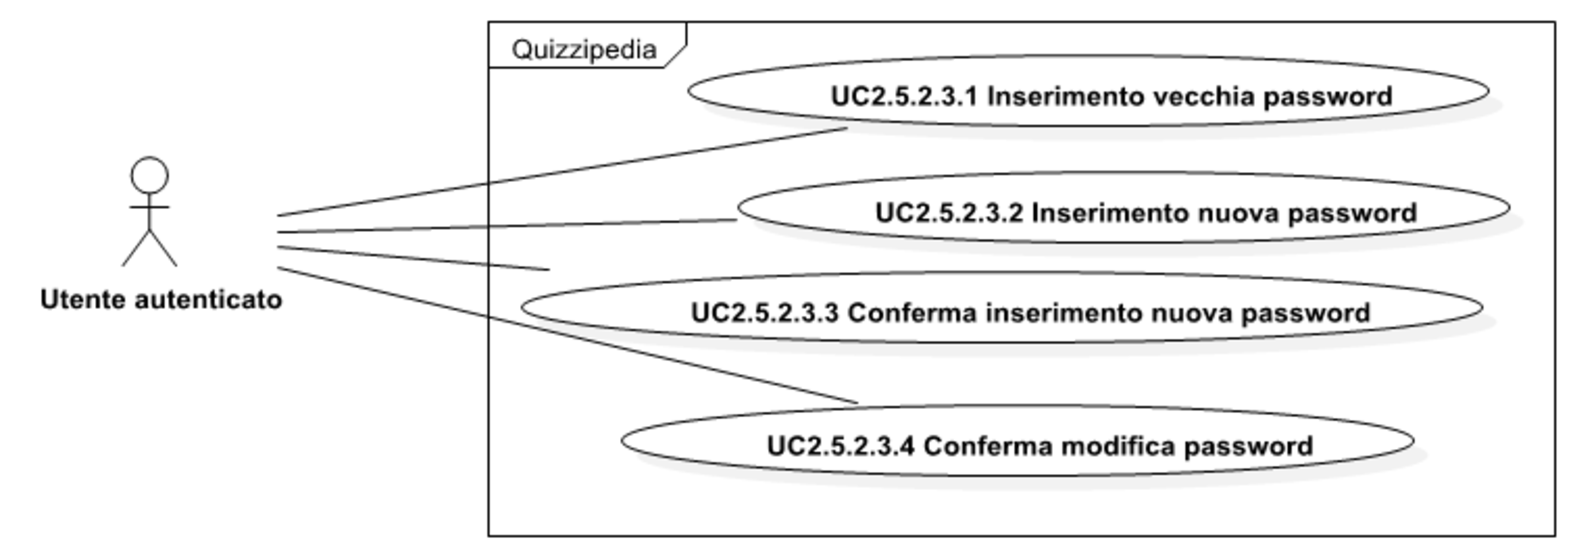
\includegraphics[width=\textwidth]{Img/UC Modifica password.pdf}}
\caption{UC2.5.2.3 Modifica password}
\end{figure}
\begin{itemize}
\item \textbf{Attori}: Utente Autenticato.
\item \textbf{Scenario principale}:
\begin{enumerate}
\item Inserimento vecchia password (UC2.5.2.3.1);
\item Inserimento nuova password (UC2.5.2.3.2);
\item Conferma inserimento nuova password (UC2.5.2.3.3);
\item Conferma modifica password (UC2.5.2.3.4).
\end{enumerate}
\item \textbf{Estensioni}:
\begin{itemize}
\item Errore modifica password (UC2.5.2.5).
\end{itemize}
\item \textbf{Descrizione}: l'utente autenticato può modificare la sua password.
\item \textbf{Precondizione}: l'utente autenticato modifica le sue informazioni personali.
\item \textbf{Postcondizione}: l'utente ha modificato la sua password.
\end{itemize}
\subsubsection{UC2.5.2.3.1 Inserimento vecchia password}
\begin{itemize}
\item \textbf{Attori}: Utente Autenticato.
\item \textbf{Descrizione}: la modifica della password richiede l'inserimento della password corrente o di una password temporanea.
\item \textbf{Precondizione}: l'utente autenticato ha deciso di modificare la password e deve ancora inserire la vecchia password.
\item \textbf{Postcondizione}: l'utente autenticato ha inserito la vecchia password.
\end{itemize}
\subsubsection{UC2.5.2.3.2 Inserimento nuova password}
\begin{itemize}
\item \textbf{Attori}: Utente Autenticato.
\item \textbf{Descrizione}: la modifica della password richiede l'inserimento della nuova password.
\item \textbf{Precondizione}: l'utente autenticato ha deciso di modificare la password e deve ancora inserire la nuova password.
\item \textbf{Postcondizione}: l'utente autenticato ha inserito la nuova password.
\end{itemize}
\subsubsection{UC2.5.2.3.3 Conferma inserimento nuova password}
\begin{itemize}
\item \textbf{Attori}: Utente Autenticato.
\item \textbf{Descrizione}: la modifica della password richiede la conferma dell'inserimento della nuova password.
\item \textbf{Precondizione}: l'utente autenticato ha deciso di modificare la password e deve ancora confermare l'inserimento della nuova password.
\item \textbf{Postcondizione}: l'utente autenticato ha confermato l'inserimento della nuova password.
\end{itemize}
\subsubsection{UC2.5.2.3.4 Conferma modifica password}
\begin{itemize}
\item \textbf{Attori}: Utente Autenticato.
\item \textbf{Descrizione}: La modifica della password richiede la conferma della modifica password.
\item \textbf{Precondizione}: l'utente autenticato ha inserito i campi necessari e deve ancora confermare la modifica della password.
\item \textbf{Postcondizione}: l'utente autenticato ha confermato la modifica della password.
\end{itemize}
\subsubsection{UC2.5.2.4 Conferma modifica informazioni personali}
\begin{itemize}
\item \textbf{Attori}: Utente Autenticato.
\item \textbf{Descrizione}: l'utente autenticato deve confermare le modifiche effettuate.
\item \textbf{Precondizione}: l'utente autenticato ha modificato qualche informazione personale.
\item \textbf{Postcondizione}: l'utente autenticato ha confermato  le nuove informazioni personali.
\end{itemize}
\subsubsection{UC2.5.2.5 Errore modifica password}
\begin{itemize}
\item \textbf{Attori}: Utente Autenticato.
\item \textbf{Descrizione}: si è verificato un errore durante la modifica della password.
\item \textbf{Precondizione}: l'utente autenticato ha inserito una password non valida.
\item \textbf{Postcondizione}: l'utente visualizza un messaggio di errore.
\end{itemize}
\subsubsection{UC2.5.3 Visualizzazione profilo quiz}
\begin{itemize}
\item \textbf{Attori}: Utente Autenticato.
\item \textbf{Descrizione}: l'utente autenticato può visualizzare il suo storico dei quiz e rivedere le risposte date.
\item \textbf{Precondizione}: l'utente autenticato può visualizzare lo storico dei quiz.
\item \textbf{Postcondizione}: l'utente ha visualizzato il suo profilo quiz.
\end{itemize}
\subsubsection{UC2.5.4 Eliminazione account utente}
\begin{itemize}
\item \textbf{Attori}: Responsabile.
\item \textbf{Generalizzazioni}:
\begin{itemize}
\item Eliminazione account personale (UC2.5.5);
\item Eliminazione altri account (UC2.5.6).
\end{itemize}
\item \textbf{Descrizione}: il responsabile può eliminare il proprio account e tutti gli account degli utenti.
\item \textbf{Precondizione}: il responsabile ha il permesso di eliminare gli account utente.
\item \textbf{Postcondizione}: il responsabile ha eliminato un account di un utente o ha eliminato il suo account.
\end{itemize}
\subsubsection{UC2.5.5 Eliminazione account personale}
\begin{itemize}
\item \textbf{Attori}: Responsabile, Utente Autenticato.
\item \textbf{Inclusioni}:
\begin{itemize}
\item Conferma eliminazione account (UC2.5.7).
\end{itemize}
\item \textbf{Descrizione}: l'utente autenticato e il responsabile possono cancellare il proprio account personale.
\item \textbf{Precondizione}: l'utente autenticato e il responsabile hanno i permessi per cancellare l'account.
\item \textbf{Postcondizione}: l'utente autenticato e il responsabile hanno selezionato il loro account per l'eliminazione.
\item \textbf{Specializzazione di}:
\begin{enumerate}
\item Eliminazione account utente (UC2.5.4).
\end{enumerate}
\end{itemize}
\subsubsection{UC2.5.6 Eliminazione altri account}
\begin{itemize}
\item \textbf{Attori}: Responsabile.
\item \textbf{Inclusioni}:
\begin{itemize}
\item Conferma eliminazione account (UC2.5.7).
\end{itemize}
\item \textbf{Descrizione}: il responsabile può cancellare gli account degli altri utenti.
\item \textbf{Precondizione}: il responsabile ha i permessi di eliminazione altri account.
\item \textbf{Postcondizione}: il responsabile ha selezionato l'account da eliminare.
\item \textbf{Specializzazione di}:
\begin{enumerate}
\item Eliminazione account utente (UC2.5.4).
\end{enumerate}
\end{itemize}
\subsubsection{UC2.5.7 Conferma eliminazione account}
\begin{itemize}
\item \textbf{Attori}: Responsabile, Utente Autenticato.
\item \textbf{Descrizione}: l'utente autenticato e il responsabile confermano l'eliminazione vera e propria dell'account precedentemente selezionato.
\item \textbf{Precondizione}: l'utente autenticato o il responsabile hanno precedentemente selezionato un account da eliminare.
\item \textbf{Postcondizione}: l'account precedentemente selezionato è stato eliminato definitivamente.
\end{itemize}
\subsubsection{UC2.6 Richiesta accettazione}
\begin{figure}[H]
\centering
\noindent\makebox[\textwidth]{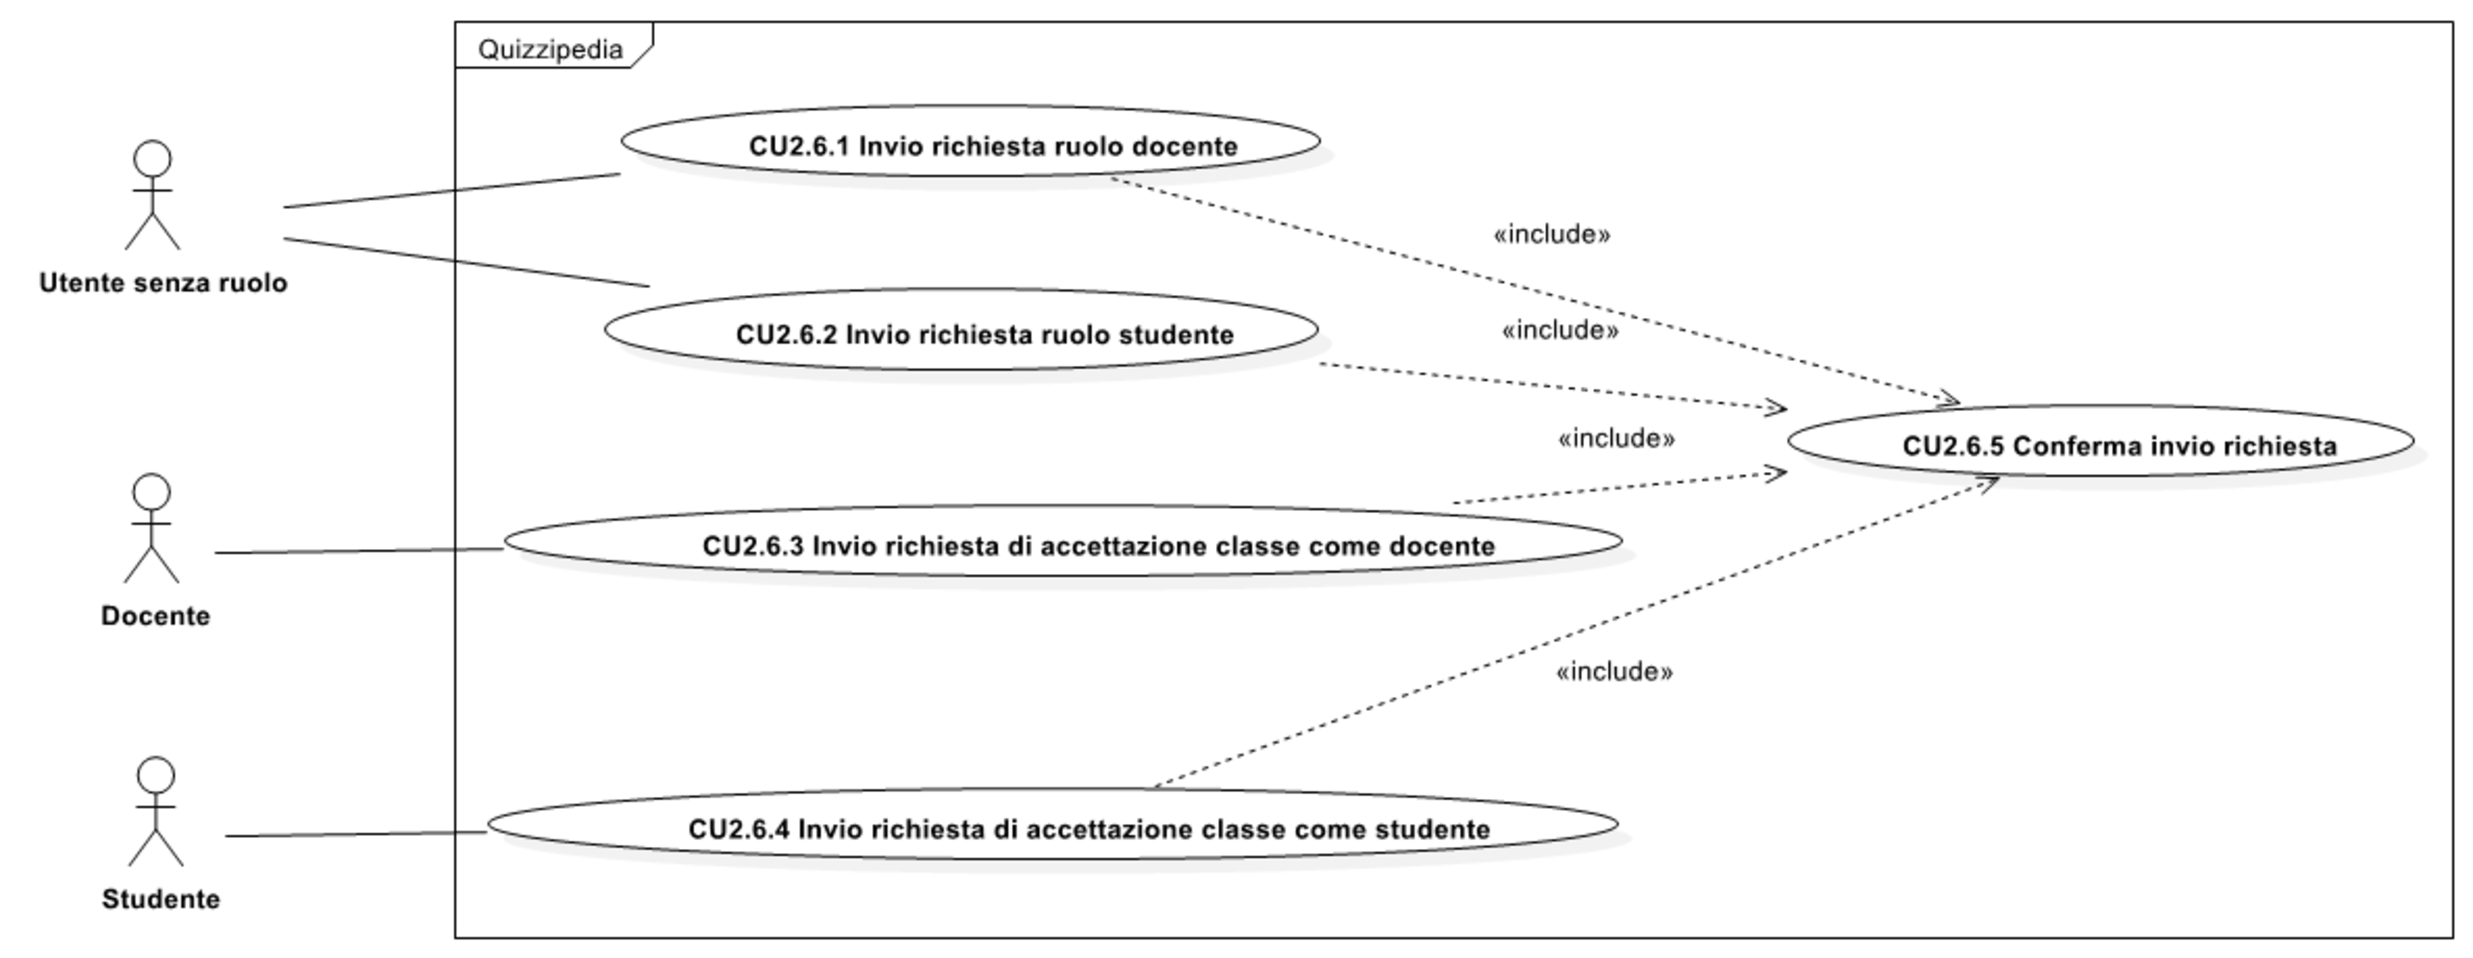
\includegraphics[width=\textwidth]{Img/UC Richiesta accettazione.pdf}}
\caption{UC2.6 Richiesta accettazione}
\end{figure}
\begin{itemize}
\item \textbf{Attori}: Docente, Studente, Utente senza Ruolo.
\item \textbf{Scenario principale}:
\begin{enumerate}
\item Invio richiesta ruolo docente (UC2.6.1);
\item Invio richiesta ruolo studente (UC2.6.2);
\item Invio richiesta di accettazione classe come docente (UC2.6.3);
\item Invio richiesta di accettazione classe come studente (UC2.6.4);
\item Conferma invio richiesta (UC2.6.5).
\end{enumerate}
\item \textbf{Descrizione}: l'utente senza ruolo invia una richiesta per essere studente o docente, mentre studente e docente inviano una richiesta di accettazione per essere inseriti in una determinata classe.
\item \textbf{Precondizione}: utente senza ruolo, studente e docente possono inviare richieste di accettazione.
\item \textbf{Postcondizione}: è stata inviata una richesta d'accettazione e sarà notificata al responsabile.
\end{itemize}
\subsubsection{UC2.6.1 Invio richiesta ruolo docente}
\begin{itemize}
\item \textbf{Attori}: Utente senza Ruolo.
\item \textbf{Inclusioni}:
\begin{itemize}
\item Conferma invio richiesta (UC2.6.5).
\end{itemize}
\item \textbf{Descrizione}: l'utente senza ruolo compila la richiesta per acquisire il ruolo di docente che sarà successivamente accettata  o rifiutata dal responsabile.
\item \textbf{Precondizione}: l'utente deve essere un utente senza ruolo.
\item \textbf{Postcondizione}: l'utente senza ruolo ha compilato la richiesta di acquisizione ruolo docente.
\end{itemize}
\subsubsection{UC2.6.2 Invio richiesta ruolo studente}
\begin{itemize}
\item \textbf{Attori}: Utente senza Ruolo.
\item \textbf{Inclusioni}:
\begin{itemize}
\item Conferma invio richiesta (UC2.6.5).
\end{itemize}
\item \textbf{Descrizione}: l'utente senza ruolo compila la richiesta per acquisire il ruolo di studente che sarà successivamente accettata o rifiutata dal responsabile.
\item \textbf{Precondizione}: l'utente deve essere un utente senza ruolo.
\item \textbf{Postcondizione}: l'utente senza ruolo ha compilato la richiesta di acquisizione ruolo studente.
\end{itemize}
\subsubsection{UC2.6.3 Invio richiesta di accettazione classe come docente}
\begin{itemize}
\item \textbf{Attori}: Docente.
\item \textbf{Scenario principale}:
\begin{enumerate}
\item Inserimento nome classe (UC2.6.3.1).
\end{enumerate}
\item \textbf{Inclusioni}:
\begin{itemize}
\item Conferma invio richiesta (UC2.6.5).
\end{itemize}
\item \textbf{Descrizione}: il docente invia una richiesta al responsabile con il nome della classe per avere il permesso di essere inserito nella classe indicata.
\item \textbf{Precondizione}: il docente ha il permesso di inviare la richiesta.
\item \textbf{Postcondizione}: il docente ha compilato la richiesta.
\end{itemize}
\subsubsection{UC2.6.3.1 Inserimento nome classe}
\begin{itemize}
\item \textbf{Attori}: Docente.
\item \textbf{Descrizione}: il docente seleziona il nome della classe alla quale vuole essere inserito.
\item \textbf{Precondizione}: il docente è nella fase di invio richiesta di accettazione classe come docente.
\item \textbf{Postcondizione}: il docente ha selezionato il nome della classe.
\end{itemize}
\subsubsection{UC2.6.4 Invio richiesta di accettazione classe come studente}
\begin{itemize}
\item \textbf{Attori}: Studente.
\item \textbf{Scenario principale}:
\begin{enumerate}
\item Inserimento nome classe (UC2.6.4.1).
\end{enumerate}
\item \textbf{Inclusioni}:
\begin{itemize}
\item Conferma invio richiesta (UC2.6.5).
\end{itemize}
\item \textbf{Descrizione}: lo studente compila invia una richiesta al responsabile con il nome della classe per avere il permesso di essere inserito nella classe indicata.
\item \textbf{Precondizione}: lo studente ha il permesso di inviare questa richiesta.
\item \textbf{Postcondizione}: lo studente ha compilato la richiesta.
\end{itemize}
\subsubsection{UC2.6.4.1 Inserimento nome classe}
\begin{itemize}
\item \textbf{Attori}: Studente.
\item \textbf{Descrizione}: lo studente seleziona il nome della classe alla quale vuole essere inserito.
\item \textbf{Precondizione}: lo studente è nella fase di invio di richiesta di accettazione classe come studente.
\item \textbf{Postcondizione}: lo studente ha selezionato il nome della classe.
\end{itemize}
\subsubsection{UC2.6.5 Conferma invio richiesta}
\begin{itemize}
\item \textbf{Attori}: Docente, Studente, Utente senza Ruolo.
\item \textbf{Descrizione}: l'utente senza ruolo, studente e docente confermano l'invio della richiesta  precedentemente compilata.
\item \textbf{Precondizione}: l'utente senza ruolo, docente, studente hanno compilato la richiesta appropriata.
\item \textbf{Postcondizione}: la richiesta è stata inviata al responsabile con successo.
\end{itemize}
\subsubsection{UC2.7 Visualizzazione statistiche}
\begin{figure}[H]
\centering
\noindent\makebox[\textwidth]{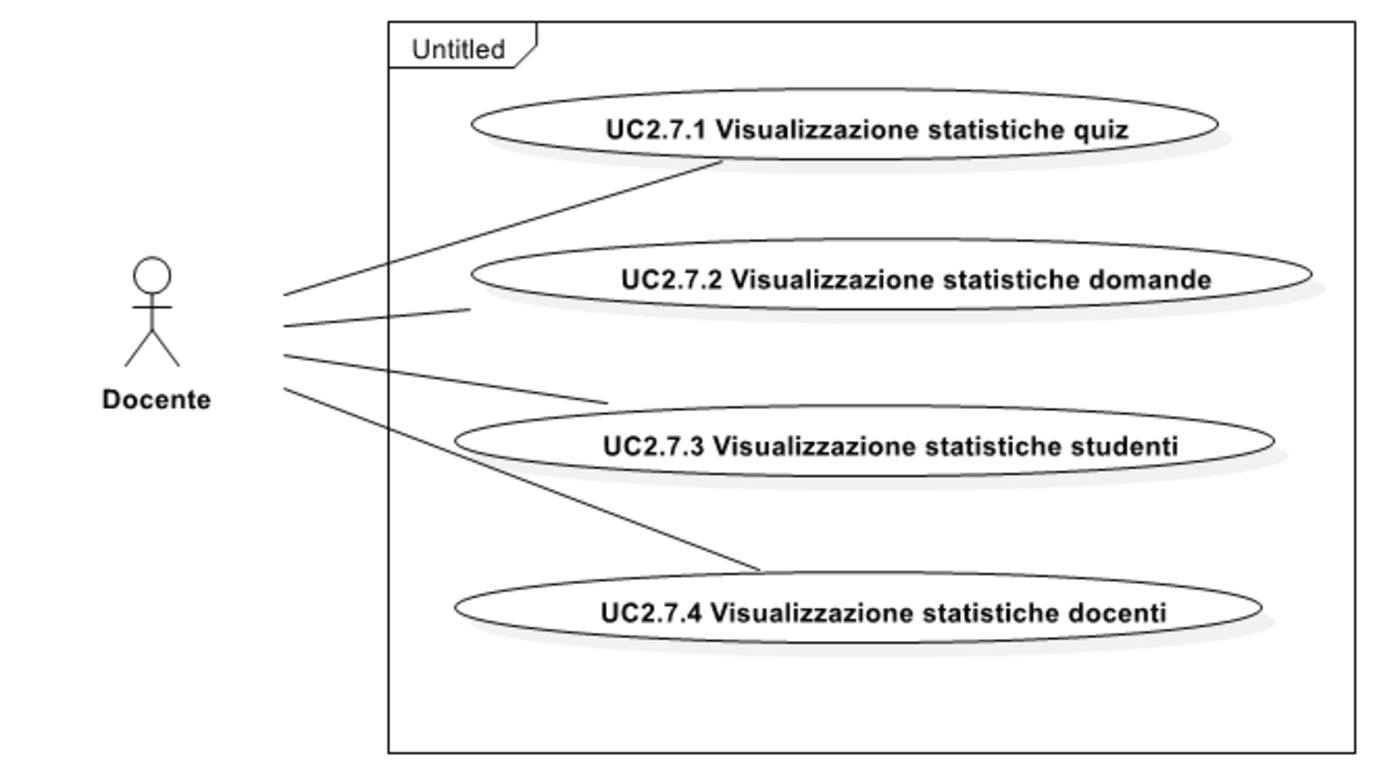
\includegraphics[width=\textwidth]{Img/UC Visualizzazione statistiche.pdf}}
\caption{UC2.7 Visualizzazione statistiche}
\end{figure}
\begin{itemize}
\item \textbf{Attori}: Docente.
\item \textbf{Scenario principale}:
\begin{enumerate}
\item Visualizzazione statistiche quiz (UC2.7.1);
\item Visualizzazione statistiche domande (UC2.7.2);
\item Visualizzazione statistiche studenti (UC2.7.3);
\item Visualizzazione statistiche docenti (UC2.7.4).
\end{enumerate}
\item \textbf{Descrizione}: il docente deve poter visualizzare statistiche di vario tipo relative a quiz, domande, studenti e altri docenti.
\item \textbf{Precondizione}: il docente è autenticato nel sistema e desidera visualizzare le statistiche.
\item \textbf{Postcondizione}: il docente ha visualizzato le statistiche.
\end{itemize}
\subsubsection{UC2.7.1 Visualizzazione statistiche quiz}
\begin{figure}[H]
\centering
\noindent\makebox[\textwidth]{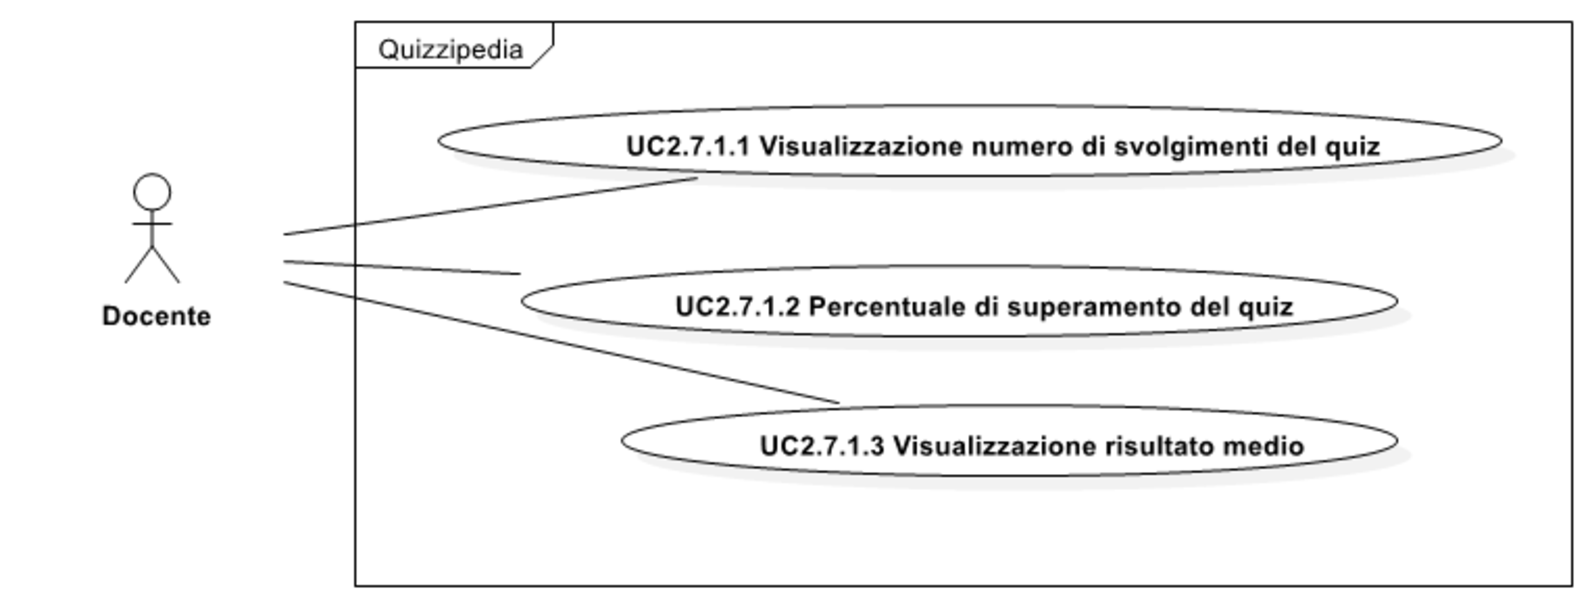
\includegraphics[width=\textwidth]{Img/UC Visualizzazione statistiche quiz.pdf}}
\caption{UC2.7.1 Visualizzazione statistiche quiz}
\end{figure}
\begin{itemize}
\item \textbf{Attori}: Docente.
\item \textbf{Scenario principale}:
\begin{enumerate}
\item Visualizzazione numero di svolgimenti (UC2.7.1.1);
\item Visualizzazione percentuale di superamento del quiz (UC2.7.1.2);
\item Visualizzazione risultato medio (UC2.7.1.3).
\end{enumerate}
\item \textbf{Descrizione}: il docente deve poter visualizzare statistiche legate ai quiz.
\item \textbf{Precondizione}: il docente è autenticato nel sistema e desidera visualizzare le statistiche legate ai quiz.
\item \textbf{Postcondizione}: il docente ha visualizzato le statistiche legate ai quiz.
\end{itemize}
\subsubsection{UC2.7.1.1 Visualizzazione numero di svolgimenti}
\begin{itemize}
\item \textbf{Attori}: Docente.
\item \textbf{Descrizione}: il docente deve poter visualizzare il numero di volte in cui un quiz è stato svolto.
\item \textbf{Precondizione}: il docente ha deciso di visualizzare le statistiche legate ai quiz.
\item \textbf{Postcondizione}: il docente ha visualizzato il numero di svolgimenti di un quiz.
\end{itemize}
\subsubsection{UC2.7.1.2 Visualizzazione percentuale di superamento del quiz}
\begin{itemize}
\item \textbf{Attori}: Docente.
\item \textbf{Descrizione}: il docente deve poter visualizzare la percentuale di studenti che hanno svolto il quiz con esito positivo.
\item \textbf{Precondizione}: il docente ha deciso di visualizzare le statistiche legate ai quiz.
\item \textbf{Postcondizione}: il docente ha visualizzato la percentuale di superamento di un quiz.
\end{itemize}
\subsubsection{UC2.7.1.3 Visualizzazione risultato medio}
\begin{itemize}
\item \textbf{Attori}: Docente.
\item \textbf{Descrizione}: il docente deve poter visualizzare il risultato medio ottenuto dagli utenti che hanno svolto il quiz.
\item \textbf{Precondizione}: il docente ha deciso di visualizzare le statistiche legate ai quiz.
\item \textbf{Postcondizione}: il docente ha visualizzato il risultato medio di un quiz.
\end{itemize}
\subsubsection{UC2.7.2 Visualizzazione statistiche domande}
\begin{figure}[H]
\centering
\noindent\makebox[\textwidth]{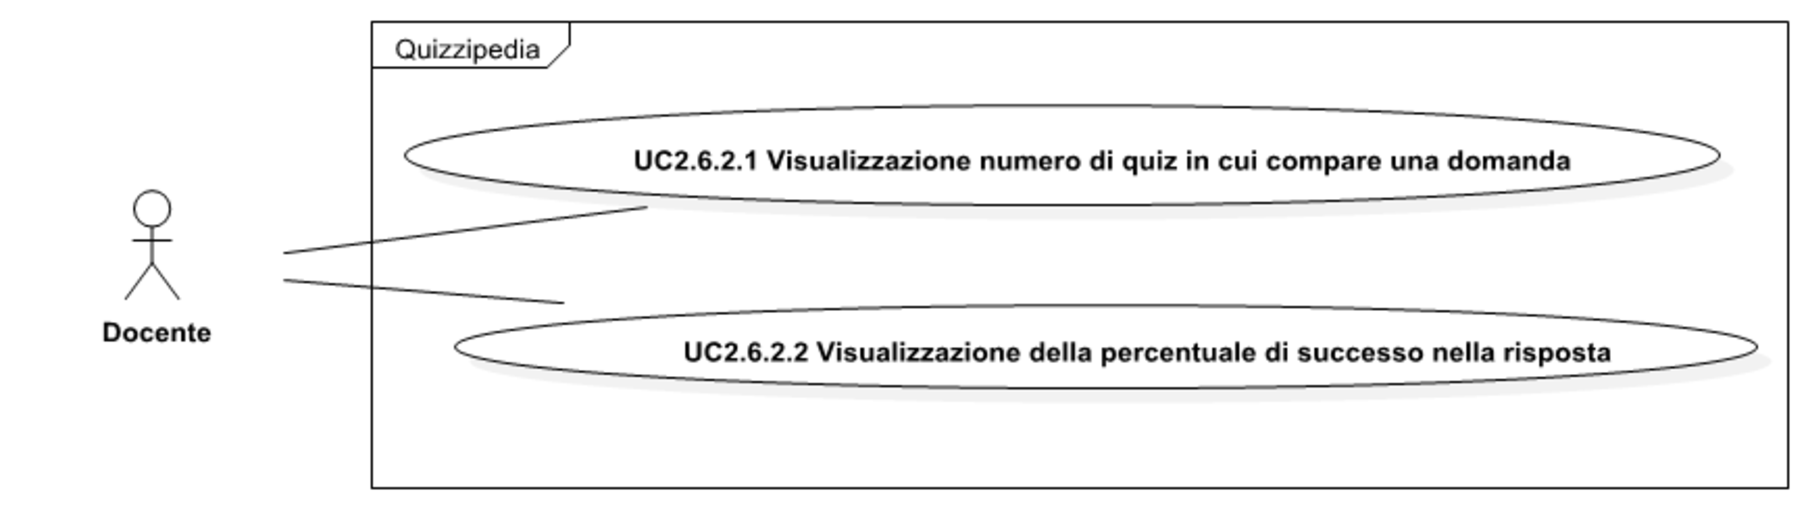
\includegraphics[width=\textwidth]{Img/UC Visualizzazione statistiche domande.pdf}}
\caption{UC2.7.2 Visualizzazione statistiche domande}
\end{figure}
\begin{itemize}
\item \textbf{Attori}: Docente.
\item \textbf{Scenario principale}:
\begin{enumerate}
\item Visualizzazione numero di quiz in cui compare una domanda (UC2.7.2.1);
\item Visualizzazione percentuale di successo nella risposta (UC2.7.2.2).
\end{enumerate}
\item \textbf{Descrizione}: il docente deve poter visualizzare statistiche legate alle domande.
\item \textbf{Precondizione}: il docente è autenticato nel sistema e desidera visualizzare le statistiche legate alle domande.
\item \textbf{Postcondizione}: il docente ha visualizzato le statistiche legate alle domande.
\end{itemize}
\subsubsection{UC2.7.2.1 Visualizzazione numero di quiz in cui compare una domanda}
\begin{itemize}
\item \textbf{Attori}: Docente.
\item \textbf{Descrizione}: il docente deve poter visualizzare il numero di quiz in cui compare la domanda.
\item \textbf{Precondizione}: il docente ha deciso di visualizzare le statistiche legate alle domande.
\item \textbf{Postcondizione}: il docente ha visualizzato il numero di quiz in cui compare una domanda.
\end{itemize}
\subsubsection{UC2.7.2.2 Visualizzazione percentuale di successo nella risposta}
\begin{itemize}
\item \textbf{Attori}: Docente.
\item \textbf{Descrizione}: il docente deve poter visualizzare la percentuale di successo nella risposta della domanda.
\item \textbf{Precondizione}: il docente ha deciso di visualizzare le statistiche legate alle domande.
\item \textbf{Postcondizione}: il docente ha visualizzato la percentuale di successo nella risposta a una domanda.
\end{itemize}
\subsubsection{UC2.7.3 Visualizzazione statistiche studenti}
\begin{figure}[H]
\centering
\noindent\makebox[\textwidth]{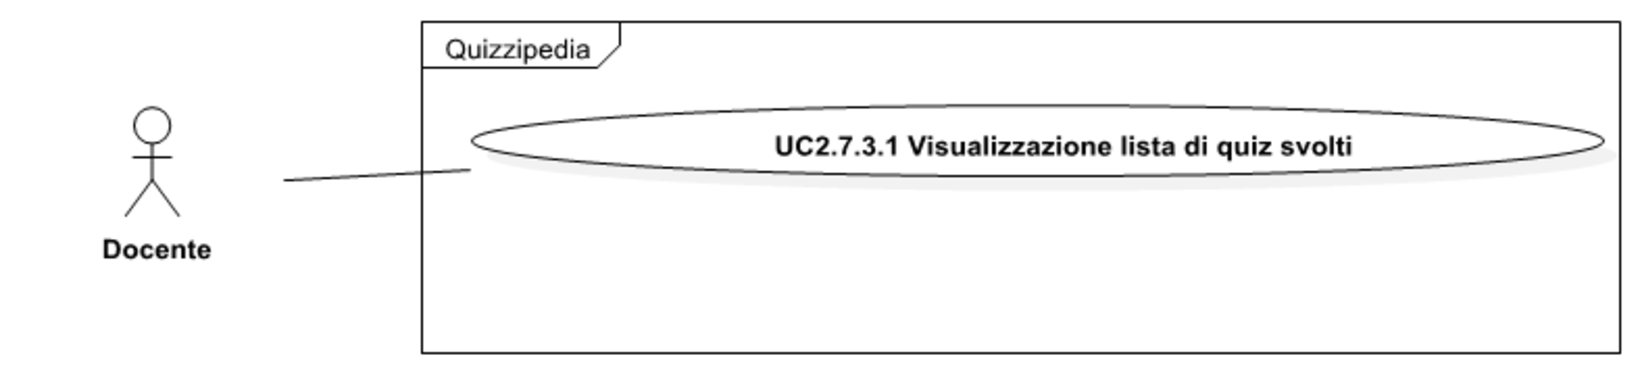
\includegraphics[width=\textwidth]{Img/UC Visualizzazione statistiche studenti.pdf}}
\caption{UC2.7.3 Visualizzazione statistiche studenti}
\end{figure}
\begin{itemize}
\item \textbf{Attori}: Docente.
\item \textbf{Scenario principale}:
\begin{enumerate}
\item Visualizzazione lista di quiz svolti (UC2.7.3.1).
\end{enumerate}
\item \textbf{Descrizione}:  il docente deve poter visualizzare statistiche legate agli studenti.
\item \textbf{Precondizione}: il docente è autenticato nel sistema e desidera visualizzare le statistiche legate agli studenti.
\item \textbf{Postcondizione}: il docente ha visualizzato le statistiche legate agli studenti.
\end{itemize}
\subsubsection{UC2.7.3.1 Visualizzazione lista di quiz svolti}
\begin{itemize}
\item \textbf{Attori}: Docente.
\item \textbf{Descrizione}: il docente deve poter visualizzare una lista dei quiz svolti dallo studente con rispettivo risultato.
\item \textbf{Precondizione}: il docente ha deciso di visualizzare le statistiche legate agli studenti.
\item \textbf{Postcondizione}: il docente ha visualizzato la lista dei quiz svolti da uno studente.
\end{itemize}
\subsubsection{UC2.7.4 Visualizzazione statistiche docenti}
\begin{figure}[H]
\centering
\noindent\makebox[\textwidth]{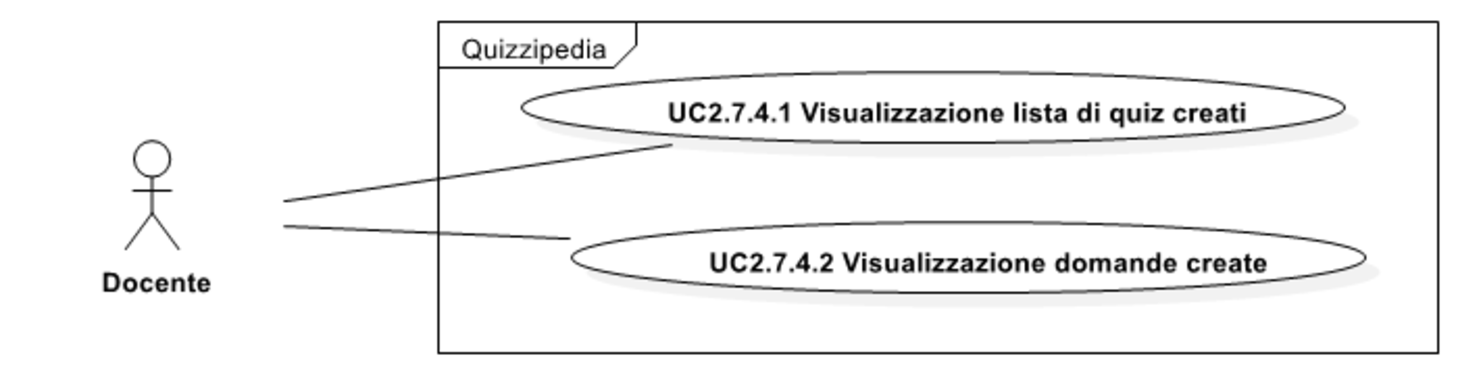
\includegraphics[width=\textwidth]{Img/UC Visualizzazione statistiche docenti.pdf}}
\caption{UC2.7.4 Visualizzazione statistiche docenti}
\end{figure}
\begin{itemize}
\item \textbf{Attori}: Docente.
\item \textbf{Scenario principale}:
\begin{enumerate}
\item Visualizzazione lista di quiz creati (UC2.7.4.1);
\item Visualizzazione lista di domande create (UC2.7.4.2).
\end{enumerate}
\item \textbf{Descrizione}: il docente deve poter visualizzare statistiche legate ai docenti.
\item \textbf{Precondizione}: il docente è autenticato nel sistema e desidera visualizzare le statistiche legate ai docenti.
\item \textbf{Postcondizione}: il docente ha visualizzato le statistiche legate ai docenti.
\end{itemize}
\subsubsection{UC2.7.4.1 Visualizzazione lista di quiz creati}
\begin{itemize}
\item \textbf{Attori}: Docente.
\item \textbf{Descrizione}: il docente deve poter visualizzare una lista dei quiz creati dal docente.
\item \textbf{Precondizione}: il docente ha deciso di visualizzare le statistiche legate ai docenti.
\item \textbf{Postcondizione}: il docente ha visualizzato la lista dei quiz creati da un docente.
\end{itemize}
\subsubsection{UC2.7.4.2 Visualizzazione lista di domande create}
\begin{itemize}
\item \textbf{Attori}: Docente.
\item \textbf{Descrizione}: il docente deve poter visualizzare una lista delle domande create dal docente.
\item \textbf{Precondizione}: il docente ha deciso di visualizzare le statistiche legate ai docenti.
\item \textbf{Postcondizione}: il docente ha visualizzato la lista delle domande create da un docente.
\end{itemize}
\subsubsection{UC2.8 Gestione enti}
\begin{figure}[H]
\centering
\noindent\makebox[\textwidth]{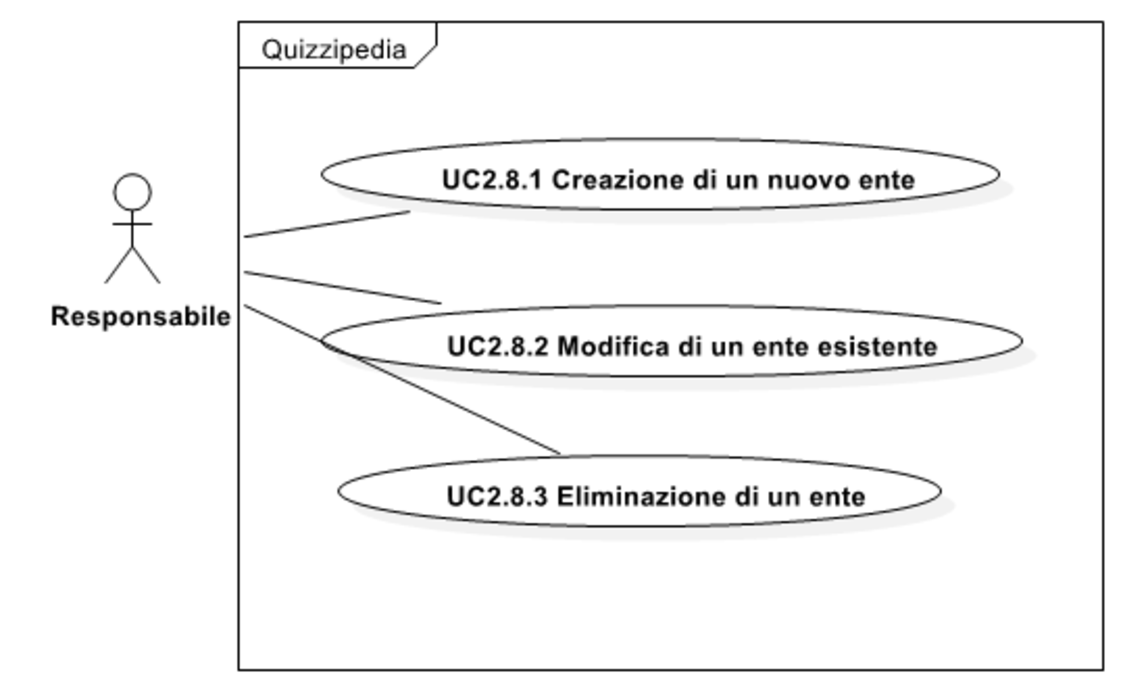
\includegraphics[width=\textwidth]{Img/UC Gestione enti.pdf}}
\caption{UC2.8 Gestione enti}
\end{figure}
\begin{itemize}
\item \textbf{Attori}: Responsabile.
\item \textbf{Scenario principale}:
\begin{enumerate}
\item Creazione di un nuovo ente (UC2.8.1);
\item Modifica di un ente esistente (UC2.8.2);
\item Eliminazione di un ente (UC2.8.3).
\end{enumerate}
\item \textbf{Descrizione}: il responsabile ha la completa gestione dell'ente di cui è a capo.
\item \textbf{Precondizione}: il responsabile ha il permesso di gestire l'ente.
\item \textbf{Postcondizione}: il responsabile potrebbe aver modificato alcune informazioni riguardante l'ente.
\end{itemize}
\subsubsection{UC2.8.1 Creazione di un nuovo ente}
\begin{figure}[H]
\centering
\noindent\makebox[\textwidth]{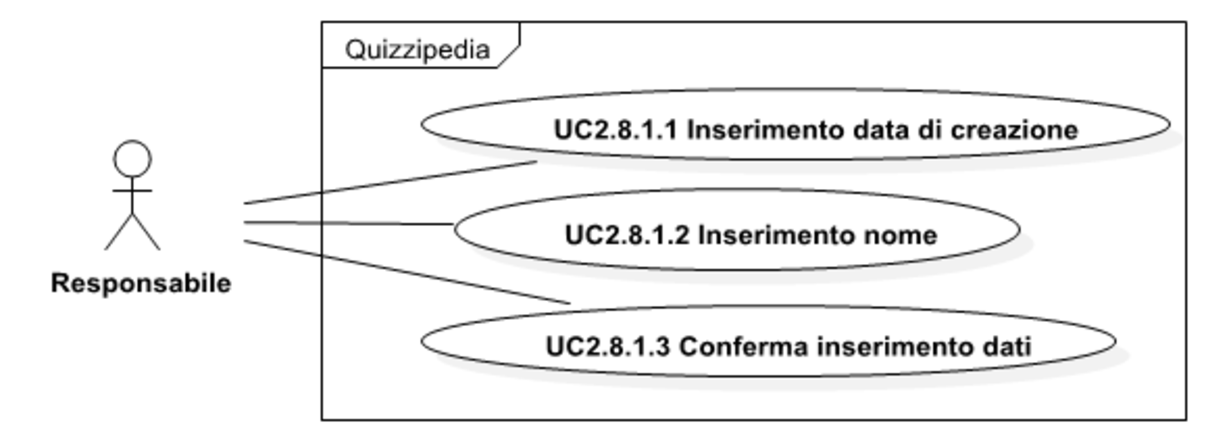
\includegraphics[width=\textwidth]{Img/UC Creazione di un nuovo ente.pdf}}
\caption{UC2.8.1 Creazione di un nuovo ente}
\end{figure}
\begin{itemize}
\item \textbf{Attori}: Responsabile.
\item \textbf{Scenario principale}:
\begin{enumerate}
\item Inserimento data di creazione (UC2.8.1.1);
\item Inserimento nome (UC2.8.1.2);
\item Conferma inserimento dati (UC2.8.1.3).
\end{enumerate}
\item \textbf{Descrizione}: il responsabile deve poter inserire un nuovo ente.
\item \textbf{Precondizione}: il responsabile ha il permesso di gestire l'ente.
\item \textbf{Postcondizione}: il responsabile ha creato un nuovo ente di cui ne è il capo.
\end{itemize}
\subsubsection{UC2.8.1.1 Inserimento data di creazione}
\begin{itemize}
\item \textbf{Attori}: Responsabile.
\item \textbf{Descrizione}: il responsabile deve poter inserisce la data di creazione dell'ente.
\item \textbf{Precondizione}: il responsabile sta creando l'ente.
\item \textbf{Postcondizione}: il responsabile ha inserito la data di creazione.
\end{itemize}
\subsubsection{UC2.8.1.2 Inserimento nome}
\begin{itemize}
\item \textbf{Attori}: Responsabile.
\item \textbf{Descrizione}:  il responsabile deve poter inserire il nome dell'ente.
\item \textbf{Precondizione}: il responsabile sta creando l'ente e deve ancora inserire il nome.
\item \textbf{Postcondizione}: il responsabile ha inserito il nome dell'ente.
\end{itemize}
\subsubsection{UC2.8.1.3 Conferma inserimento dati}
\begin{itemize}
\item \textbf{Attori}: Responsabile.
\item \textbf{Descrizione}: il responsabile conferma i dati precedentemente inseriti per avviare la creazione dell'ente.
\item \textbf{Precondizione}: il responsabile sta creando l'ente e deve ancora confermare i dati inseriti.
\item \textbf{Postcondizione}: i dati precedentemente inseriti sono stati confermati e l'ente è stato creato.
\end{itemize}
\subsubsection{UC2.8.2 Modifica di un ente esistente}
\begin{figure}[H]
\centering
\noindent\makebox[\textwidth]{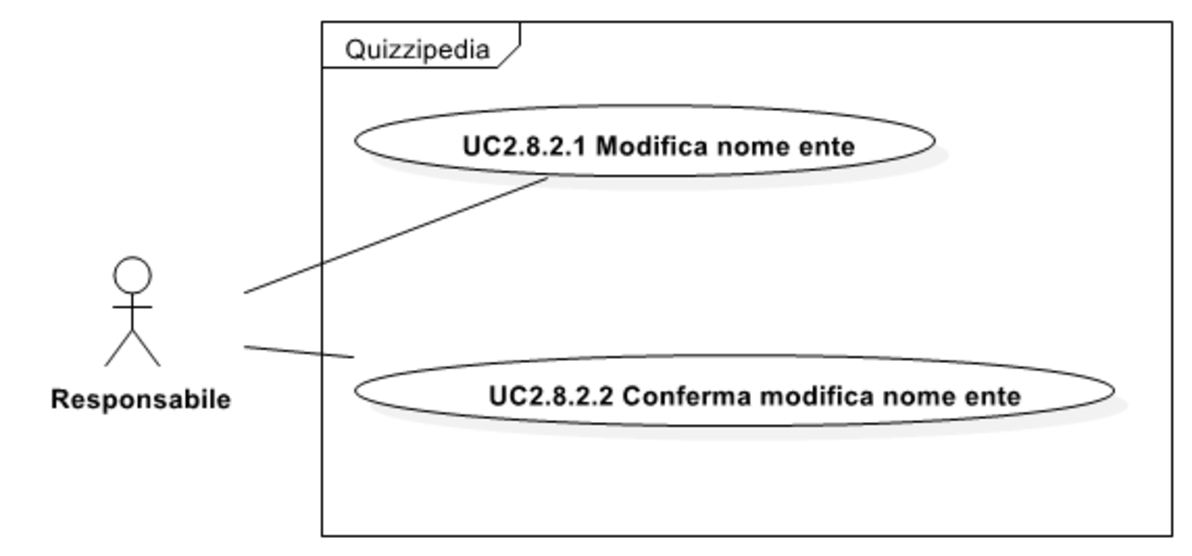
\includegraphics[width=\textwidth]{Img/UC Modifica di un ente esistente.pdf}}
\caption{UC2.8.2 Modifica di un ente esistente}
\end{figure}
\begin{itemize}
\item \textbf{Attori}: Responsabile.
\item \textbf{Scenario principale}:
\begin{enumerate}
\item Modifica nome ente (UC2.8.2.1);
\item Conferma modifica ente (UC2.8.2.2).
\end{enumerate}
\item \textbf{Descrizione}: il responsabile deve poter modificare i dati dell'ente che ha precedentemente creato.
\item \textbf{Precondizione}: il responsabile ha il permesso di modificare le informazioni dell'ente.
\item \textbf{Postcondizione}: il responsabile ha modificato le informazioni dell'ente.
\end{itemize}
\subsubsection{UC2.8.2.1 Modifica nome ente}
\begin{itemize}
\item \textbf{Attori}: Responsabile.
\item \textbf{Descrizione}: il responsabile deve poter modificare il nome dell'ente.
\item \textbf{Precondizione}: il responsabile sta modificando i dati dell'ente e vuole modificare il nome.
\item \textbf{Postcondizione}: il responsabile ha modificato il nome dell'ente.
\end{itemize}
\subsubsection{UC2.8.2.2 Conferma modifica ente}
\begin{itemize}
\item \textbf{Attori}: Responsabile.
\item \textbf{Descrizione}: il responsabile deve confermare la modifica dell'ente.
\item \textbf{Precondizione}: il responsabile ha modificando i dati dell'ente e deve ancora confermare le modifiche fatte.
\item \textbf{Postcondizione}: il responsabile ha confermato le modifiche effettuate.
\end{itemize}
\subsubsection{UC2.8.3 Eliminazione di un ente}
\begin{figure}[H]
\centering
\noindent\makebox[\textwidth]{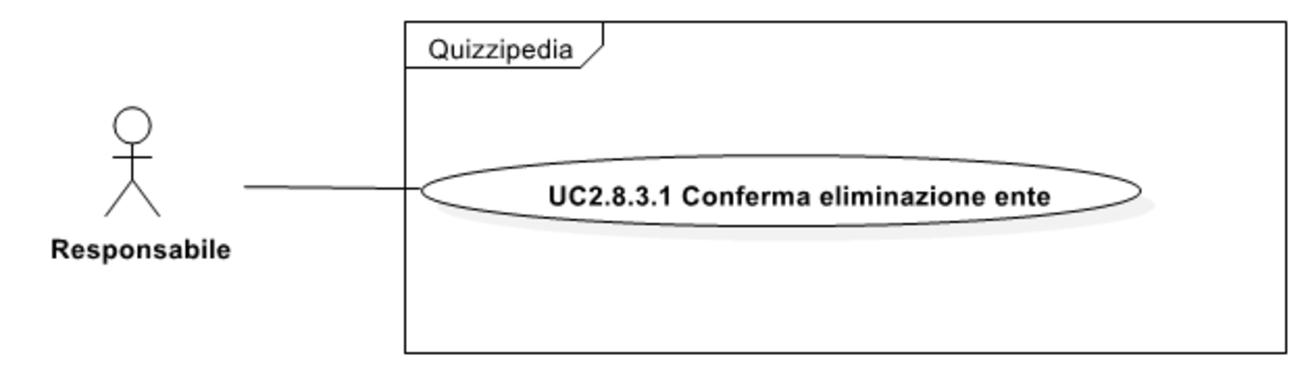
\includegraphics[width=\textwidth]{Img/UC Eliminazione di un ente.pdf}}
\caption{UC2.8.3 Eliminazione di un ente}
\end{figure}
\begin{itemize}
\item \textbf{Attori}: Responsabile.
\item \textbf{Scenario principale}:
\begin{enumerate}
\item Conferma eliminazione ente (UC2.8.3.1).
\end{enumerate}
\item \textbf{Descrizione}: il responsabile deve poter eliminare un ente di cui è proprietario.
\item \textbf{Precondizione}: il responsabile è nella gestione degli enti e vuole eliminare un suo ente.
\item \textbf{Postcondizione}: il responsabile ha eliminato l'ente.
\end{itemize}
\subsubsection{UC2.8.3.1 Conferma eliminazione ente}
\begin{itemize}
\item \textbf{Attori}: Responsabile.
\item \textbf{Descrizione}: il responsabile deve confermare l'eliminazione dell'ente.
\item \textbf{Precondizione}: il responsabile ha scelto un ente da eliminare e deve ancora confermare.
\item \textbf{Postcondizione}: il responsabile ha confermato l'ente da eliminare.
\end{itemize}
\subsubsection{UC2.9 Gestione classe}
\begin{figure}[H]
\centering
\noindent\makebox[\textwidth]{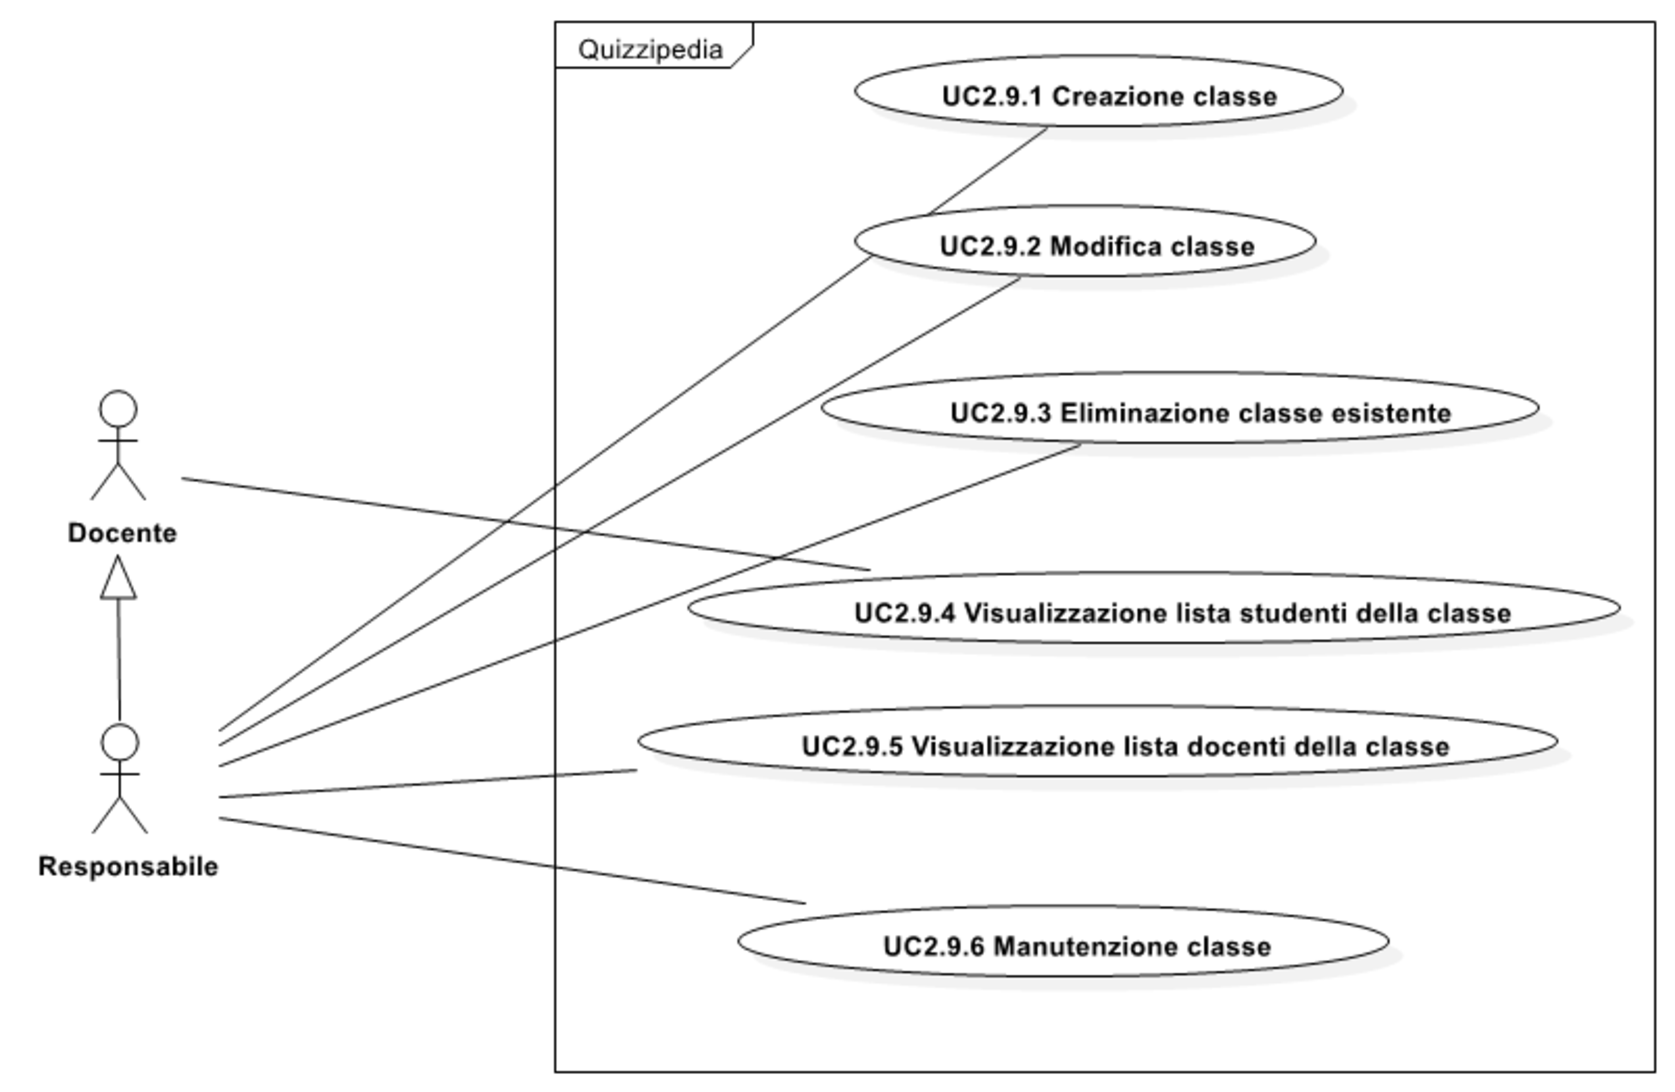
\includegraphics[width=\textwidth]{Img/UC Gestione classe.pdf}}
\caption{UC2.9 Gestione classe}
\end{figure}
\begin{itemize}
\item \textbf{Attori}: Responsabile.
\item \textbf{Scenario principale}:
\begin{enumerate}
\item Creazione classe (UC2.9.1);
\item Modifica classe (UC2.9.2);
\item Eliminazione classe esistente (UC2.9.3);
\item Visualizza lista studenti della classe (UC2.9.4);
\item Visualizza lista docenti della classe (UC2.9.5);
\item Manutenzione classe (UC2.9.6).
\end{enumerate}
\item \textbf{Descrizione}: il responsabile può creare, modificare ed elimanare una classe; inoltre può visualizzare la lista degli studenti e docenti delle classe; può fare manutenzione sulle classi nel caso in cui le richieste di inserimento da parte di studenti e docenti fossero sbagliate; infine gestisce la lista delle richiesta che riceve da parte degli studenti e docenti.
\item \textbf{Precondizione}: il responsabile ha i permessi per gestire le classi.
\item \textbf{Postcondizione}: il responsabile ha effettuato le operazioni di gestione delle classi.
\end{itemize}
\subsubsection{UC2.9.1 Creazione classe}
\begin{figure}[H]
\centering
\noindent\makebox[\textwidth]{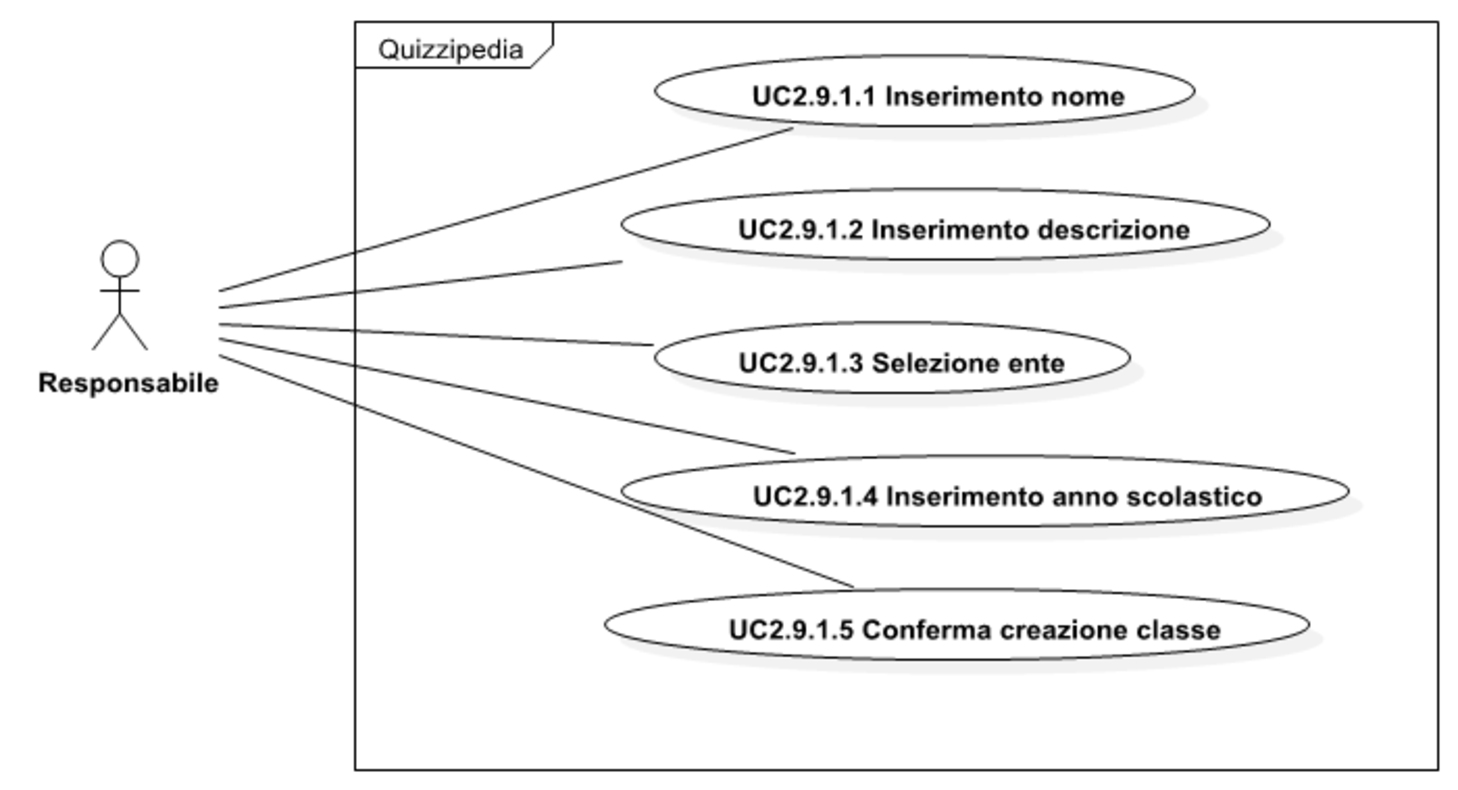
\includegraphics[width=\textwidth]{Img/UC Creazione classe.pdf}}
\caption{UC2.9.1 Creazione classe}
\end{figure}
\begin{itemize}
\item \textbf{Attori}: Responsabile.
\item \textbf{Scenario principale}:
\begin{enumerate}
\item Inserimento nome (UC2.9.1.1);
\item Inserimento descrizione (UC2.9.1.2);
\item Selezione ente (UC2.9.1.3);
\item Inserimento anno scolastico (UC2.9.1.4);
\item Conferma creazione classe (UC2.9.1.5).
\end{enumerate}
\item \textbf{Descrizione}: il responsabile deve poter creare una classe.
\item \textbf{Precondizione}: il responsabile ha i permessi per creare una classe ed è nella gestione classe.
\item \textbf{Postcondizione}: il responsabile ha creato una nuova classe.
\end{itemize}
\subsubsection{UC2.9.1.1 Inserimento nome}
\begin{itemize}
\item \textbf{Attori}: Responsabile.
\item \textbf{Descrizione}: il responsabile deve poter inserisce il nome della classe.
\item \textbf{Precondizione}: il responsabile sta creando una classe e deve ancora inserire il nome.
\item \textbf{Postcondizione}: il responsabile ha inserito il nome della classe.
\end{itemize}
\subsubsection{UC2.9.1.2 Inserimento descrizione}
\begin{itemize}
\item \textbf{Attori}: Responsabile.
\item \textbf{Descrizione}: il responsabile può inserisce una breve descrizione della classe.
\item \textbf{Precondizione}: il responsabile sta creando una classe e deve ancora inserire la descrizione.
\item \textbf{Postcondizione}: il responsabile ha inserito una breve descrizione della classe.
\end{itemize}
\subsubsection{UC2.9.1.3 Selezione ente}
\begin{itemize}
\item \textbf{Attori}: Responsabile.
\item \textbf{Descrizione}: il responsabile deve selezionare l'ente che sarà il proprietario della classe.
\item \textbf{Precondizione}: il responsabile sta creando una classe e deve ancora selezionare l'ente.
\item \textbf{Postcondizione}: il responsabile ha selezionato l'ente proprietario della classe.
\end{itemize}
\subsubsection{UC2.9.1.4 Inserimento anno scolastico}
\begin{itemize}
\item \textbf{Attori}: Responsabile.
\item \textbf{Descrizione}: il responsabile deve inserisce l'anno scolastico in cui è stata creata la classe.
\item \textbf{Precondizione}: il responsabile sta creando una classe e deve ancora inserire l'anno scolastico.
\item \textbf{Postcondizione}: il responsabile ha inserito l'anno scolastico della classe.
\end{itemize}
\subsubsection{UC2.9.1.5 Conferma creazione classe}
\begin{itemize}
\item \textbf{Attori}: Responsabile.
\item \textbf{Descrizione}: il responsabile deve confermare i dati precedentemente inseriti.
\item \textbf{Precondizione}: il responsabile ha inserito una nuova classe e deve ancora confermarla.
\item \textbf{Postcondizione}: il responsabile ha confermato i dati inseriti e la classe è stata creata.
\end{itemize}
\subsubsection{UC2.9.2 Modifica classe}
\begin{figure}[H]
\centering
\noindent\makebox[\textwidth]{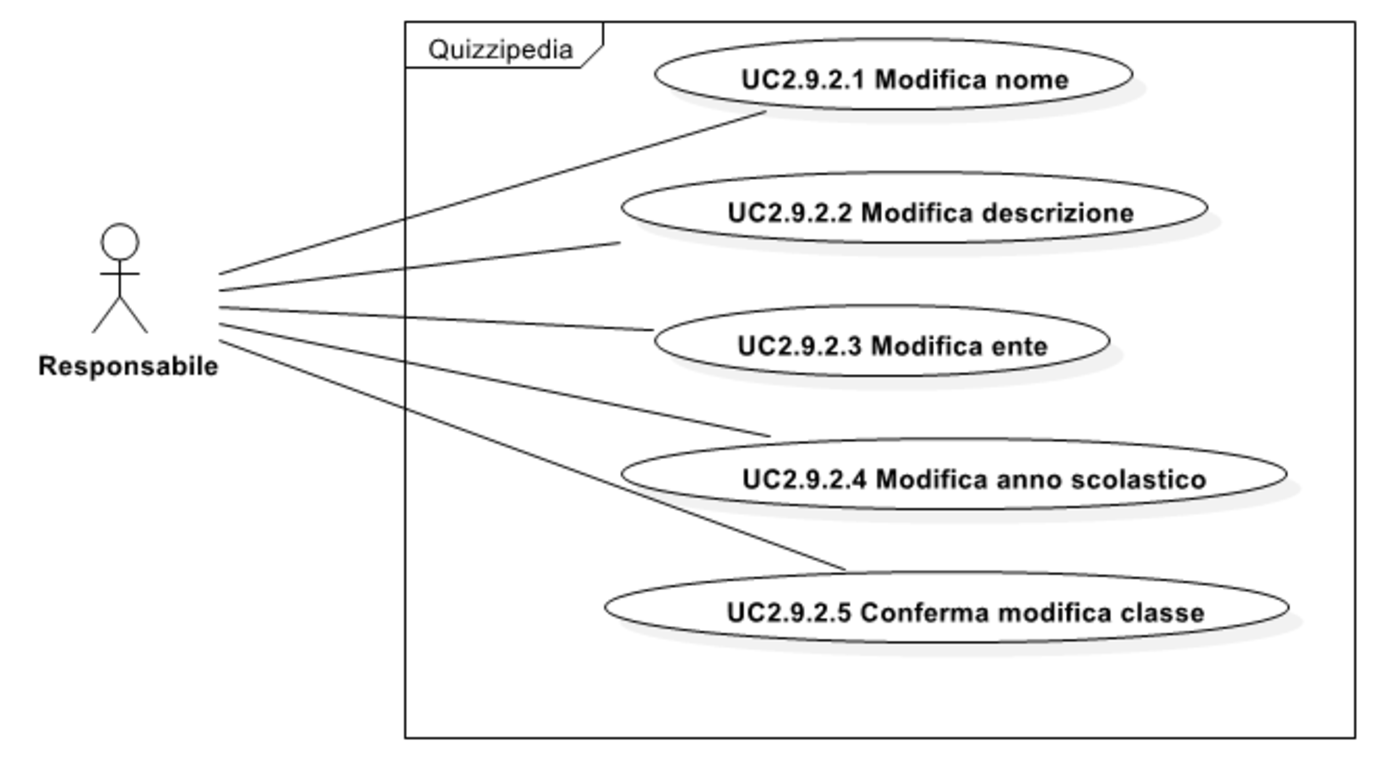
\includegraphics[width=\textwidth]{Img/UC Modifica classe.pdf}}
\caption{UC2.9.2 Modifica classe}
\end{figure}
\begin{itemize}
\item \textbf{Attori}: Responsabile.
\item \textbf{Scenario principale}:
\begin{enumerate}
\item Modifica nome (UC2.9.2.1);
\item Modifica descrizione (UC2.9.2.2);
\item Modifica ente (UC2.9.2.3);
\item Modifica anno scolastico (UC2.9.2.4);
\item Conferma modifica classe (UC2.9.2.5).
\end{enumerate}
\item \textbf{Descrizione}: il responsabile deve poter modificare i dati della classe.
\item \textbf{Precondizione}: il responsabile ha i permessi per modificare una classe.
\item \textbf{Postcondizione}: il responsabile ha effettuato le modifiche sulla classe.
\end{itemize}
\subsubsection{UC2.9.2.1 Modifica nome}
\begin{itemize}
\item \textbf{Attori}: Responsabile.
\item \textbf{Descrizione}: il responsabile deve poter modificare il nome della classe.
\item \textbf{Precondizione}: il responsabile sta modificando la classe.
\item \textbf{Postcondizione}: il responsabile ha modificato il nome della classe.
\end{itemize}
\subsubsection{UC2.9.2.2 Modifica descrizione}
\begin{itemize}
\item \textbf{Attori}: Responsabile.
\item \textbf{Descrizione}: il responsabile deve poter modificare la descrizione della classe.
\item \textbf{Precondizione}: il responsabile sta modificando la classe.
\item \textbf{Postcondizione}: il responsabile ha modificato la descrizione della classe.
\end{itemize}
\subsubsection{UC2.9.2.3 Modifica ente}
\begin{itemize}
\item \textbf{Attori}: Responsabile.
\item \textbf{Descrizione}: il responsabile deve poter modificare l'ente della classe a cui è associata.
\item \textbf{Precondizione}: il responsabile sta modificando la classe.
\item \textbf{Postcondizione}: il responsabile ha modificato l'ente della classe.
\end{itemize}
\subsubsection{UC2.9.2.4 Modifica anno scolastico}
\begin{itemize}
\item \textbf{Attori}: Responsabile.
\item \textbf{Descrizione}: il responsabile deve poter modificare l'anno scolastico della creazione della classe.
\item \textbf{Precondizione}: il responsabile sta modificando la classe.
\item \textbf{Postcondizione}: il responsabile ha modificato l'anno scolastico della classe.
\end{itemize}
\subsubsection{UC2.9.2.5 Conferma modifica classe}
\begin{itemize}
\item \textbf{Attori}: Responsabile.
\item \textbf{Descrizione}: il responsabile deve confermare le modifiche precedentemente fatte.
\item \textbf{Precondizione}: il responsabile ha modificato la classe e deve ancora confermare le modifiche.
\item \textbf{Postcondizione}: il responsabile ha confermato le modifiche.
\end{itemize}
\subsubsection{UC2.9.3 Eliminazione classe esistente}
\begin{figure}[H]
\centering
\noindent\makebox[\textwidth]{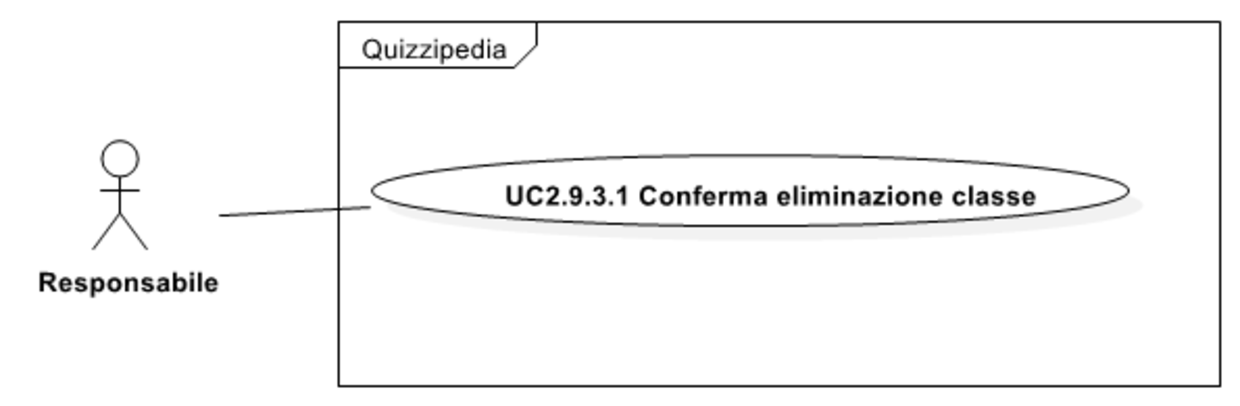
\includegraphics[width=\textwidth]{Img/UC Eliminazione classe esistente.pdf}}
\caption{UC2.9.3 Eliminazione classe esistente}
\end{figure}
\begin{itemize}
\item \textbf{Attori}: Responsabile.
\item \textbf{Scenario principale}:
\begin{enumerate}
\item Conferma eliminazione classe (UC2.9.3.1).
\end{enumerate}
\item \textbf{Descrizione}: il responsabile può eliminare una classe.
\item \textbf{Precondizione}: il responsabile ha i permessi per eliminare una classe.
\item \textbf{Postcondizione}: il responsabile ha eliminato la classe.
\end{itemize}
\subsubsection{UC2.9.3.1 Conferma eliminazione classe}
\begin{itemize}
\item \textbf{Attori}: Responsabile.
\item \textbf{Descrizione}: il responsabile deve confermare l'eliminazione della classe.
\item \textbf{Precondizione}: il responsabile vuole eliminare una classe e deve ancora confermare.
\item \textbf{Postcondizione}: il responsabile ha confermato l'eliminazione della classe.
\end{itemize}
\subsubsection{UC2.9.4 Visualizza lista studenti della classe}
\begin{itemize}
\item \textbf{Attori}: Docente, Responsabile.
\item \textbf{Descrizione}: il responsabile e il docente selezionano il nome della classe e visualizzeranno una lista di studenti associati a quella classe.
\item \textbf{Precondizione}: il responsabile e il docente hanno il permesso di consultare la lista degli studenti.
\item \textbf{Postcondizione}: vengono visualizzati gli studenti della classe selezionata.
\end{itemize}
\subsubsection{UC2.9.5 Visualizza lista docenti della classe}
\begin{itemize}
\item \textbf{Attori}: Responsabile.
\item \textbf{Descrizione}: il responsabile e il docente selezionano il nome della classe e visualizzeranno una lista di docenti associati a quella classe.
\item \textbf{Precondizione}: il responsabile ha il permesso di consultare la lista dei docenti.
\item \textbf{Postcondizione}: il responsabile visualizza i docenti della classe selezionata.
\end{itemize}
\subsubsection{UC2.9.6 Manutenzione classe}
\begin{figure}[H]
\centering
\noindent\makebox[\textwidth]{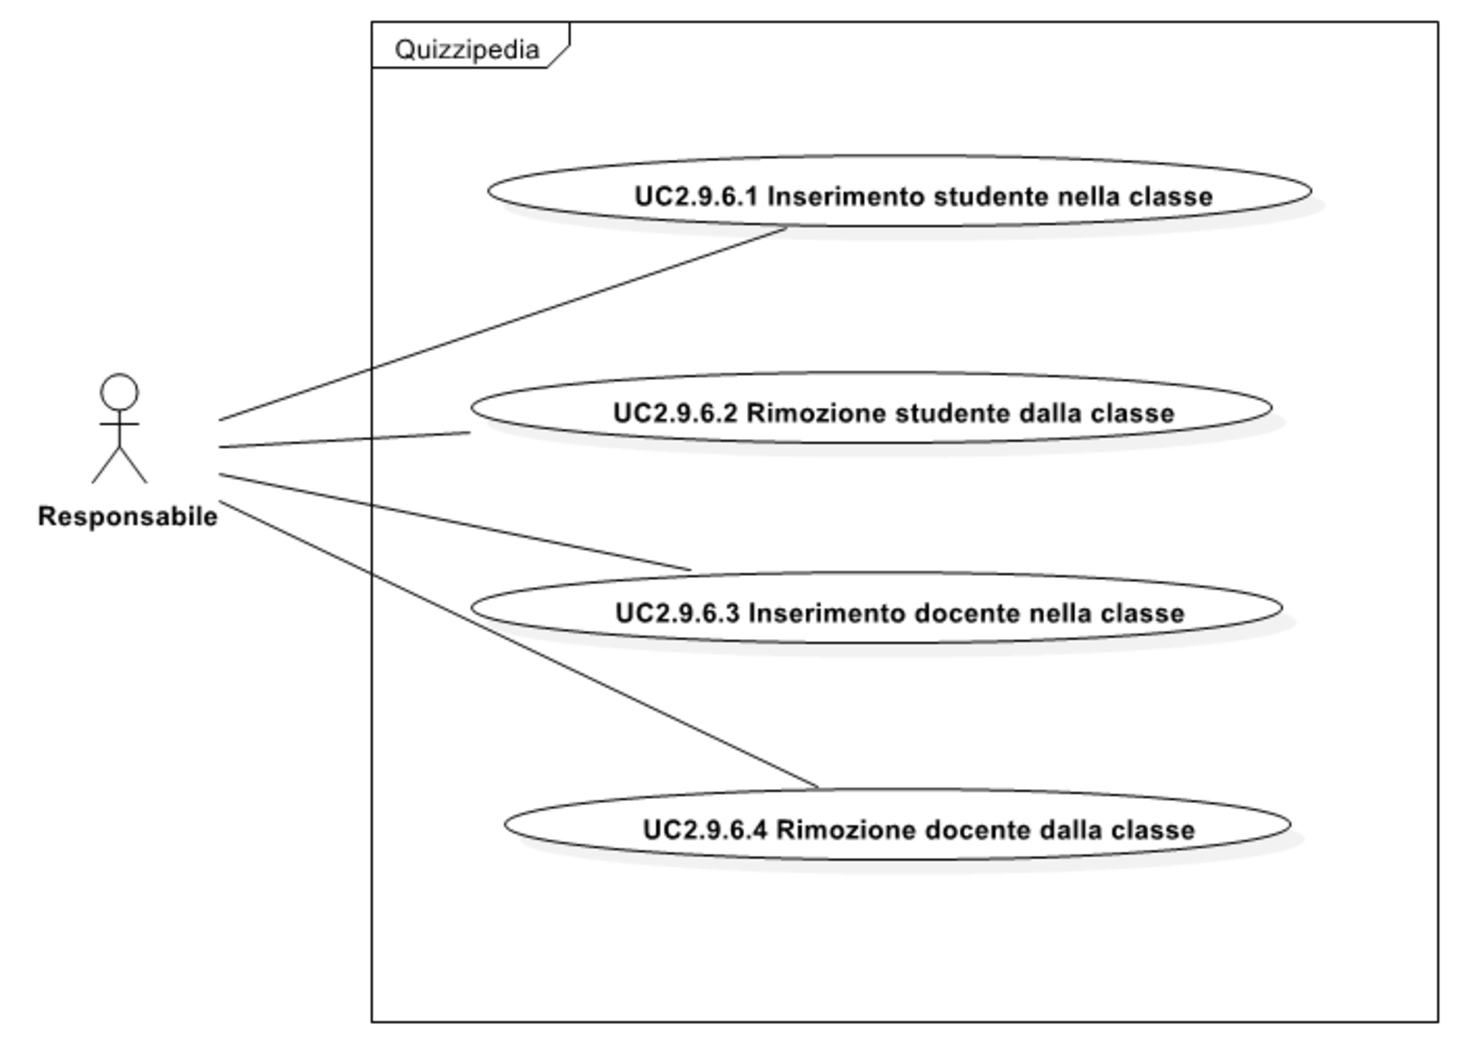
\includegraphics[width=\textwidth]{Img/UC Manutenzione classe.pdf}}
\caption{UC2.9.6 Manutenzione classe}
\end{figure}
\begin{itemize}
\item \textbf{Attori}: Responsabile.
\item \textbf{Scenario principale}:
\begin{enumerate}
\item Inserimento studente nella classe (UC2.9.6.1);
\item Rimozione studente dalla classe (UC2.9.6.2);
\item Inserimento docente nella classe (UC2.9.6.3);
\item Rimozione docente dalla classe (UC2.9.6.4).
\end{enumerate}
\item \textbf{Descrizione}: il responsabile può fare manutenzione su una classe nel caso in cui uno studente o un docente si sia inscritto in una classe sbagliata. Il responsabile procederà alla rimozione con successivo inserimento dello studente o del docente nella classe corretta.
\item \textbf{Precondizione}: il responsabile ha il permesso di fare manutenzione alla classe.
\item \textbf{Postcondizione}: il responsabile ha fatto alcune operazioni di manutenzione alla classe.
\end{itemize}
\subsubsection{UC2.9.6.1 Inserimento studente nella classe}
\begin{itemize}
\item \textbf{Attori}: Responsabile.
\item \textbf{Descrizione}: il responsabile può inserire uno studente nella classe.
\item \textbf{Precondizione}: il responsabile ha deciso di effettuare la manutenzione della classe.
\item \textbf{Postcondizione}: il responsabile ha inserito lo studente nella classe.
\end{itemize}
\subsubsection{UC2.9.6.2 Rimozione studente dalla classe}
\begin{itemize}
\item \textbf{Attori}: Responsabile.
\item \textbf{Descrizione}: il responsabile può rimuovere uno studente dalla classe.
\item \textbf{Precondizione}: il responsabile ha deciso di effettuare la manutenzione della classe.
\item \textbf{Postcondizione}: il responsabile ha rimosso lo studente dalla classe.
\end{itemize}
\subsubsection{UC2.9.6.3 Inserimento docente nella classe}
\begin{itemize}
\item \textbf{Attori}: Responsabile.
\item \textbf{Descrizione}: il responsabile può inserire un docente nella classe.
\item \textbf{Precondizione}: il responsabile ha deciso di effettuare la manutenzione della classe.
\item \textbf{Postcondizione}: il responsabile ha inserito il docente nella classe.
\end{itemize}
\subsubsection{UC2.9.6.4 Rimozione docente dalla classe}
\begin{itemize}
\item \textbf{Attori}: Responsabile.
\item \textbf{Descrizione}: il responsabile può rimuovere un docente dalla classe.
\item \textbf{Precondizione}: il responsabile ha deciso di effettuare la modifica della classe.
\item \textbf{Postcondizione}: il responsabile ha rimosso il docente dalla classe.
\end{itemize}
\subsubsection{UC2.10 Lista richieste}
\begin{figure}[H]
\centering
\noindent\makebox[\textwidth]{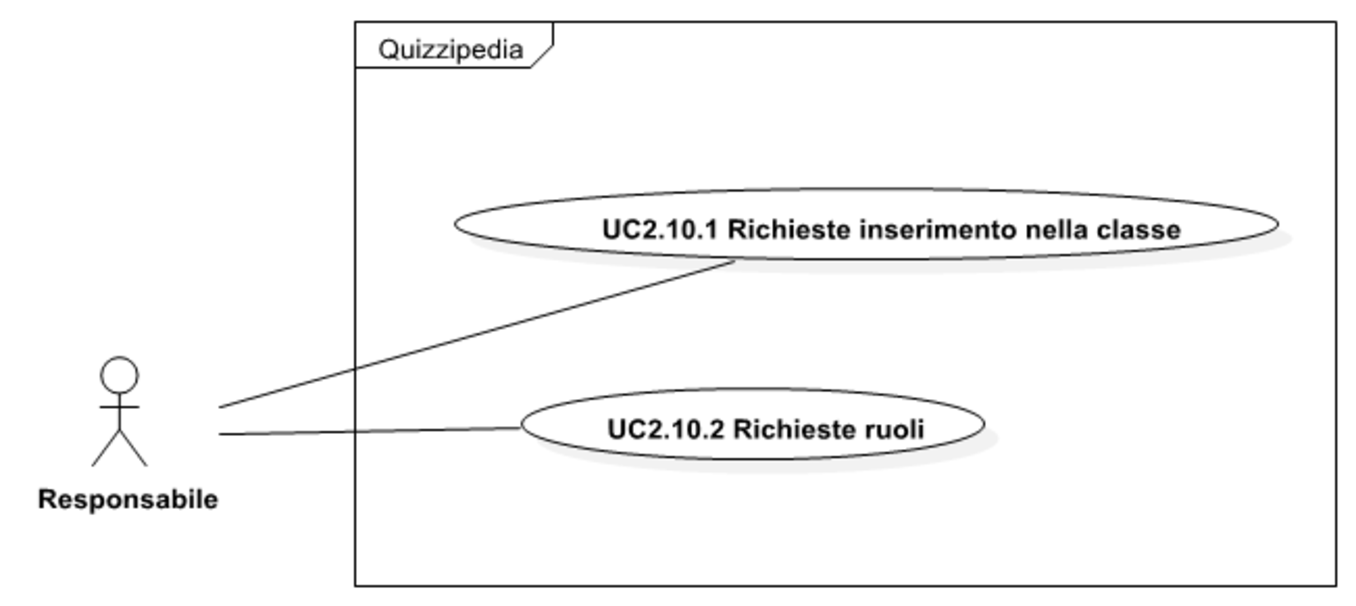
\includegraphics[width=\textwidth]{Img/UC Lista richieste.pdf}}
\caption{UC2.10 Lista richieste}
\end{figure}
\begin{itemize}
\item \textbf{Attori}: Responsabile.
\item \textbf{Scenario principale}:
\begin{enumerate}
\item Richieste inserimento nella classe (UC2.10.1);
\item Richieste ruoli (UC2.10.2).
\end{enumerate}
\item \textbf{Descrizione}: il responsabile gestisce le richieste inviate da studenti, docenti ed utenti senza ruolo per accettare o annullare il ruolo richiesto o per accettare e annullare l'inserimento dello studente o docente in una determinata classe.
\item \textbf{Precondizione}: il responsabile ha i permessi per la gestione delle richieste.
\item \textbf{Postcondizione}: il responsabile ha accettato o rifiutato alcune richieste che ha ricevuto.
\end{itemize}
\subsubsection{UC2.10.1 Richieste inserimento nella classe}
\begin{figure}[H]
\centering
\noindent\makebox[\textwidth]{\includegraphics[width=\textwidth]{Img/UC Richieste inserimento nella classe.pdf}}
\caption{UC2.10.1 Richieste inserimento nella classe}
\end{figure}
\begin{itemize}
\item \textbf{Attori}: Responsabile.
\item \textbf{Scenario principale}:
\begin{enumerate}
\item Accettazione della richiesta di inserimento (UC2.10.1.1);
\item Annullamento della richiesta di inserimento (UC2.10.1.2).
\end{enumerate}
\item \textbf{Descrizione}: il responsabile accetta o rifiuta le richieste di inserimento nella classe ricevute dagli studenti e docenti.
\item \textbf{Precondizione}: il responsabile visualizza la lista di richieste di inserimento nella classe.
\item \textbf{Postcondizione}: il responsabile ha accettato o rifiutato le richieste che ha ricevuto.
\end{itemize}
\subsubsection{UC2.10.1.1 Accettazione della richiesta di inserimento}
\begin{itemize}
\item \textbf{Attori}: Responsabile.
\item \textbf{Descrizione}: il responsabile accetta le richieste di inserimento nella classe ricevute dagli studenti e docenti.
\item \textbf{Precondizione}: il responsabile visualizza lista richieste di inserimento nella classe.
\item \textbf{Postcondizione}: il responsabile ha accettato le richieste di inserimento nella classe che gli sono pervenute dagli studenti e docenti.
\end{itemize}
\subsubsection{UC2.10.1.2 Annullamento della richiesta di inserimento}
\begin{itemize}
\item \textbf{Attori}: Responsabile.
\item \textbf{Descrizione}: il responsabile rifiuta le richieste di inserimento nella classe ricevute dagli studenti e docenti.
\item \textbf{Precondizione}: il responsabile visualizza lista richieste di inserimento nella classe.
\item \textbf{Postcondizione}: il responsabile ha rifiutato le richieste di inserimento nella classe che gli sono pervenute dagli studenti e docenti.
\end{itemize}
\subsubsection{UC2.10.2 Richieste ruoli}
\begin{figure}[H]
\centering
\noindent\makebox[\textwidth]{\includegraphics[width=\textwidth]{Img/UC Richieste ruoli.pdf}}
\caption{UC2.10.2 Richieste ruoli}
\end{figure}
\begin{itemize}
\item \textbf{Attori}: Responsabile.
\item \textbf{Scenario principale}:
\begin{enumerate}
\item Accettazione del ruolo (UC2.10.2.1);
\item Annullamento richiesta ruolo (UC2.10.2.2).
\end{enumerate}
\item \textbf{Descrizione}: il responsabile accetta o rifiuta le richieste  del ruolo che vogliono assumere gli utenti senza ruolo.
\item \textbf{Precondizione}: il responsabile ha i permessi per la gestione della lista richieste.
\item \textbf{Postcondizione}: il responsabile ha accettato o rifiutato le richieste dei ruoli che gli sono pervenute dagli utenti senza ruolo.
\end{itemize}
\subsubsection{UC2.10.2.1 Accettazione del ruolo}
\begin{itemize}
\item \textbf{Attori}: Responsabile.
\item \textbf{Descrizione}: il responsabile accetta  le richieste  del ruolo che vogliono assumere gli utenti senza ruolo.
\item \textbf{Precondizione}: il responsabile visualizza la lista richieste ruoli.
\item \textbf{Postcondizione}: il responsabile ha accettato le richieste del ruolo che gli sono pervenute dagli utenti senza ruolo.
\end{itemize}
\subsubsection{UC2.10.2.2 Annullamento richiesta ruolo}
\begin{itemize}
\item \textbf{Attori}: Responsabile.
\item \textbf{Descrizione}: il responsabile rifiuta le richieste  del ruolo che vogliono assumere gli utenti senza ruolo.
\item \textbf{Precondizione}: il responsabile visualizza la lista richieste ruoli.
\item \textbf{Postcondizione}: il responsabile ha rifiutato le richieste del ruolo che gli sono pervenute dagli utenti senza ruolo.
\end{itemize}